% =============================================================================
% STANDALONE PAPER 1 of 4 -- Pillar 1: GRPO Scaling Laws
% Reuses shared preamble/author/methods; pulls the P1 section family + frontier synthesis.
% Build: pdflatex paper_P1_scaling ; bibtex paper_P1_scaling ; pdflatex x2
% =============================================================================
\documentclass{article}
\usepackage{tikz}
\usetikzlibrary{shapes,arrows.meta,positioning,calc}
% Shared preamble for the 4 per-pillar papers (extracted from main.tex)
% NeurIPS 2026 style (download from https://neurips.cc)
% \usepackage{neurips_2025}       % For camera-ready
\usepackage[preprint,nonatbib]{neurips_2026} % For preprint (remove for submission)
\usepackage[numbers]{natbib}
% \usepackage[nonatbib]{neurips_2026} % Submission mode (anonymized, line numbers)

\usepackage{iftex}
\ifPDFTeX
  \usepackage[utf8]{inputenc}
\fi
\usepackage[T1]{fontenc}
\usepackage{hyperref}
\usepackage{url}
\usepackage{booktabs}
\usepackage{amsfonts}
\usepackage{amsmath}
\usepackage{amssymb}
\usepackage{nicefrac}
\usepackage{microtype}
\usepackage{xcolor}
\usepackage{graphicx}
\usepackage{subcaption}
\usepackage{algorithm}
\usepackage{algorithmic}
\usepackage{multirow}
\usepackage{siunitx}
\usepackage{listings}
\usepackage{enumitem}
\usepackage{tikz}
\usetikzlibrary{positioning, fit, arrows.meta, backgrounds, calc, shadows, shapes.geometric, shapes.misc, decorations.pathreplacing}

% Custom commands
\newcommand{\tinker}{\textsc{Tinker}}
\newcommand{\atropos}{\textsc{Atropos}}
\newcommand{\grpo}{\textsc{Grpo}}
\newcommand{\ours}{\textsc{TinkerRL-Bench}}
% Custom command for partial answers in NeurIPS checklist
\newcommand{\answerPartial}[1][]{\textcolor{purple}{[Partial] #1}}

% Helper macros used by the section files (define here so the per-pillar papers are self-contained)
\providecommand{\eps}{\ensuremath{\epsilon}}
\providecommand{\tableref}[1]{Table~\ref{#1}}
\providecommand{\secref}[1]{Section~\ref{#1}}
\providecommand{\paragraphref}[1]{Paragraph~\ref{#1}}
\providecommand{\figref}[1]{Figure~\ref{#1}}
\providecommand{\eqnref}[1]{Eq.~\eqref{#1}}

% Resolve both explicit paths and the canonical figures/ directory before
% degrading to a visible missing-artifact box. \IfFileExists alone does not
% honor \graphicspath, which previously hid checked-in figures in pillar PDFs.
\usepackage{letltxmacro}
\LetLtxMacro{\origincludegraphics}{\includegraphics}
\renewcommand{\includegraphics}[2][]{%
  \IfFileExists{#2}{\origincludegraphics[#1]{#2}}%
  {\IfFileExists{figures/#2}{\origincludegraphics[#1]{figures/#2}}%
  {\fbox{\parbox{0.7\linewidth}{\centering\small\textit{[missing figure artifact: \texttt{\detokenize{#2}}]}}}}}}

% Math operators + stray Unicode math chars used by some sections
\DeclareMathOperator*{\argmax}{arg\,max}
\DeclareMathOperator*{\argmin}{arg\,min}
\ifdefined\DeclareUnicodeCharacter
\DeclareUnicodeCharacter{0394}{\ensuremath{\Delta}}
\DeclareUnicodeCharacter{03B4}{\ensuremath{\delta}}
\DeclareUnicodeCharacter{00D7}{\ensuremath{\times}}
\DeclareUnicodeCharacter{2264}{\ensuremath{\leq}}
\DeclareUnicodeCharacter{2265}{\ensuremath{\geq}}
\DeclareUnicodeCharacter{2248}{\ensuremath{\approx}}
\fi

% Expectation + grouping-variable name macros used by the length-bias sections
\newcommand{\E}{\mathbb{E}}
\newcommand{\task}{\textsf{task}}
\newcommand{\algo}{\textsf{algo}}
\newcommand{\seed}{\textsf{seed}}

% Further section-local macros (undefined upstream): plateau time, ZVF shorthand, signature
\newcommand{\tplat}{T_{\text{plat}}}
\newcommand{\zvf}{\ensuremath{\widetilde{\mathrm{ZVF}}}}
\providecommand{\signature}{\ensuremath{\mathcal{S}}}

% More upstream-undefined macros
\newcommand{\etal}{\emph{et al.}}
\newcommand{\note}[1]{\footnote{#1}}

% Resolve both figures/X.pdf and bare X.pdf references
\graphicspath{{figures/}{./}}

% Must load last: literal prose/path underscores occur throughout the inherited
% section corpus. Extend the package defaults only for label and natbib's
% first-string commands; do not wrap \includegraphics, whose optional width
% argument is numeric rather than a string token.
\newcommand{\UnderscoreCommands}{\do\label \do\citep \do\citet}
\usepackage[strings]{underscore}

\title{Limits of Scaling Laws for GRPO Post-Training:\\
       Execution-Substrate Variance and Cross-Scale Horizons up to 1\,T Parameters}
% Shared author block --- INDIVIDUAL (solo) M.Tech project
\author{
  Arvind C R \\
  PES University\\
  \texttt{arvindcr4@gmail.com} \\
  \And
  Ramesh Prakash Guledgudd\thanks{Project guide.} \\
  PES University\\
  \texttt{rameshpg@pes.edu} \\
}

\begin{document}
\sloppy \hbadness=10000 \vbadness=10000 \hfuzz=2pt
\maketitle
% Pillar-1 (scaling) standalone abstract
\begin{abstract}
Group Relative Policy Optimization (GRPO) has become a default algorithm for
reinforcement-learning (RL) post-training of language models, yet how its benefit
scales with model size remains unclear and is easily confounded by implementation
and evaluation choices. We study GRPO scaling as one pillar of \ours{}, combining
(i)~an execution-substrate and library audit spanning 70+ total runs ($N=42$ cross-task ANOVA runs)
across seven RL implementations on a deterministic 199-action modular-arithmetic environment
and two LLM post-training back-ends (\textsc{Tinker} API and HuggingFace \textsc{TRL} on Modal A10G GPUs)
across five model families ($0.5$B--$1$T total parameters) on GSM8K, 5-choice arithmetic, and multi-hop tool-use tasks, and
(ii)~a cross-scale GRPO scaling-law audit on GSM8K across 12 open-weight checkpoints ($4$B--$1$T total parameters,
comprising 5 dense and 7 Mixture-of-Experts models) executed on the \textsc{Tinker} platform.
Crucially, the frontier-scale anchors (Qwen3-235B-MoE, DeepSeek-V3.1 at $671$B/$685$B total parameters,
Kimi-K2-Thinking at $1$T, and Nemotron-3-Super-120B-A12B LatentMoE with $12$B active parameters) are obtained through the \textsc{Tinker} managed
training/inference API in a single-seed, descriptive-only regime, which makes a
cross-scale study tractable without owning frontier hardware (and why full
base weights are not released for those anchors).
Our central result is a conservative negative one: across the $2.4$ orders of
magnitude in parameter count spanned by the 12-anchor GSM8K pool ($4$B--$1$T),
the cross-scale slope of the mean GRPO training
reward shows no reliable positive trend---flat within the wide uncertainty of
these single-seed anchors, which we read \emph{descriptively}
rather than as a powered significance test---and no single saturation exponent is identifiable
(four of the five core frontier-scale traces have their saturation rate pinned at the
$\lambda=10$ fit boundary because instruction-tuned checkpoints start near their GSM8K ceiling at step~1, and AICc model selection prefers a one-parameter constant model on all five).
On the seven full per-step traces, no run follows a clean slow-start /
rapid-rise / plateau template, and the Nemotron-120B LatentMoE run
is better described as a distinct collapse phase (zero-reward step fraction $0.55$
versus $\le 0.067$ on the other core anchors) than as a point on a smooth trend. The defensible
object is therefore a local, stack-conditioned description of endpoint levels,
which separate by step-1 baseline reward more cleanly than by $\log_{10} N$,
not a Chinchilla-style power law in $N$.
\paragraph{Venue claim boundary (workshop-short / limits audit).}
This manuscript is submitted as a \emph{descriptive limits and identifiability
audit}, not as a positive scaling law or a multi-seed cross-scale significance
study. Frontier anchors remain single-seed and descriptive by design; matched
multi-seed cross-scale runs are an explicitly stated \emph{non-claim} for this
submission and do not gate the negative/identifiability result we headline.
We release all code, logs, per-step telemetry, and trained adapters; full base-model
checkpoints are shared where model licensing permits, while the managed
frontier-scale runs expose logs and telemetry rather than base weights.
\end{abstract}
\paragraph{August 2026 evidence boundary.} This limits audit does not pool
heterogeneous checkpoints as scaling replications or infer a capacity ceiling;
only named source cells support the descriptive rows.

% Pillar-1 (scaling) standalone introduction + related work
\section{Introduction}
\label{sec:p1-intro}
Reinforcement learning from verifiable rewards has become a standard final stage
in training reasoning-capable language models, and GRPO~\citep{shao2024deepseekmath, guo2025deepseekr1} is now one of its most widely used algorithms. GRPO replaces
the learned value function of PPO~\citep{schulman2017proximal} with a
group-relative baseline: for each prompt it samples a group of $G$ completions,
scores them with a verifier, and centers the rewards within the group to form
advantages. Because it removes the critic, GRPO is cheap to run at scale, and a
natural question follows: \emph{how does the benefit of GRPO post-training change
as the base model grows?}

Pre-training exhibits smooth power-law scaling in parameter count and data
\citep{kaplan2020scalinglaws, hoffmann2022chinchilla}, and it is tempting to expect
an analogous law for RL post-training. Evidence here is thinner and more
contested~\citep{hilton2023rlscaling, rafailov2024rlhfscaling, nimmaturi2025predictive},
in part because RL gains are entangled with the rollout stack, reward parser,
reference policy, and evaluation protocol, so cross-paper comparisons conflate the
algorithm with its plumbing. This paper isolates the scaling question inside a
single, fixed benchmark.

We study GRPO scaling as one pillar of \ours{}, a controlled benchmark spanning 70+ runs
($N=42$ cross-task ANOVA runs) across seven RL implementations on a 199-choice modular-arithmetic task,
two LLM post-training back-ends (\textsc{Tinker} and HuggingFace \textsc{TRL}) across five model families ($0.5$B--$1$T total parameters)
on GSM8K~\citep{cobbe2021training}, 5-choice arithmetic, and multi-hop tool-use tasks, and a 12-anchor cross-scale GRPO suite ($4$B--$1$T) on GSM8K.
Rather than assert a new law, we report what the data will and will not
support. Our contributions are: (i) a same-benchmark measurement showing that the
cross-scale mean training-reward slope ($+0.056 \pm 0.130$/decade on 5 core anchors; $+0.081 \pm 0.129$/decade on 12 anchors) and endpoint ceiling slope ($R_{\max} \sim \log_{10} N$) are statistically indistinguishable from zero
over the measured $2.4$-decade parameter range ($p \ge 0.22$); (ii) an internal falsification check of a clean
three-phase saturation hypothesis~\citep{nimmaturi2025predictive}; (iii) an identifiability audit showing that no
universal saturation rate $\lambda$ or horizon $t_{80}$ is estimable on 20--30 step GSM8K traces because instruction-tuned checkpoints start near their ceiling at step~1 ($R(1) \in [0.75, 0.94]$), leaving a local, stack-conditioned taxonomy of endpoint ceilings separated by initial instruction-following capability rather than $\log_{10} N$; and (iv) a case study of the Nemotron-3-Super-120B-A12B (LatentMoE, $12$B active) collapse as a
distinct format-starvation phase rather than trend noise. We read single-seed frontier-API runs as
illustrative case studies, not universal laws. The title's ``limits'' is therefore
substantive: this paper identifies where a parameter-count scaling law is not
estimable from short-horizon GSM8K traces; it does not claim that GRPO lacks scaling behavior on harder, unsaturated benchmarks (e.g., AIME or competition code). The program's stronger explanatory candidates are usable
contrastive compute and group-size-conditioned signal, tested separately in the
ZVF and group-size companion papers~\citep{zvfaudit2026}.

\subsection{Related Work}
\label{sec:p1-related}
Neural scaling laws for pre-training are well established~\citep{kaplan2020scalinglaws, hoffmann2022chinchilla, muennighoff2023datascaling}. Scaling behavior of RL and
RLHF post-training has been examined more recently~\citep{hilton2023rlscaling, gao2023reward, rafailov2024rlhfscaling, nimmaturi2025predictive, tan2025scalingrl}, but typically within a single
stack, leaving open whether reported trends transfer across libraries and model
families. GRPO and its use in reasoning models originate
with~\citet{shao2024deepseekmath} and~\citet{guo2025deepseekr1};
\citet{ahmadian2024backtobasics} and~\citet{li2026oxrl} argue that much of the benefit of heavy RL
machinery is recoverable by simpler estimators once the stack is controlled.
Concurrently, recent RLVR studies have shown that group-relative updates suffer from gradient starvation when prompts yield all-correct or all-incorrect rollouts, motivating dynamic sampling in DAPO~\citep{yu2025dapo}, variance-unbiased normalization in Dr.\ GRPO~\citep{tong2025drgrpo}, online difficulty filtering~\citep{bae2025online, jiang2025vcrl}, and zero-variance prompt recycling~\citep{le2025rlzvp, zhang2026greso}.
Our work connects this variance-starvation mechanism directly to post-training scaling laws: when frontier instruction-tuned checkpoints start near saturation on GSM8K, high rollout-level zero-variance fractions flatten single-trace learning curves and mask cross-scale parameter trends.

% Shared methods (benchmark, setup, statistics) extracted from main.tex
\section{Benchmark Design}
\label{sec:benchmark}
% =============================================================================

% Task-coverage taxonomy (graphic is a task tree, not a library tree)
\begin{figure}[t]
\centering
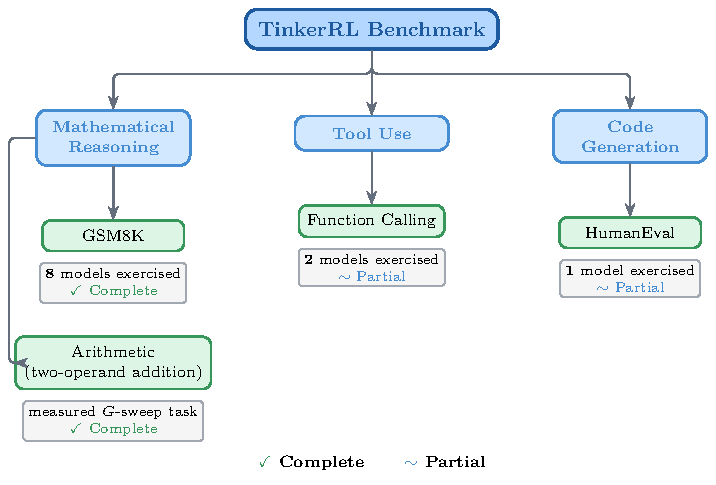
\includegraphics[width=0.85\textwidth]{tikz/taxonomy.pdf}
\caption{Task-coverage taxonomy of \ours{}. The broader benchmark organises tasks into
mathematical reasoning (GSM8K and modular arithmetic; complete and the primary focus of this scaling study), tool use / function calling
(partial), and code generation (HumanEval; partial). Library coverage is
listed separately in Table~\ref{tab:implementations}.}
\label{fig:taxonomy}
\end{figure}

\subsection{Task Suite}

% Table of tasks
\begin{table}[htbp]
\centering
\caption{Full \ours{} benchmark task suite with standardized reward functions. This paper analyzes the online RL math reasoning tracks (Math RL Arithmetic across 7 classic-RL libraries and Math RL GSM8K across 12 LLM scale anchors); the SFT, DPO, and distillation tracks are evaluated in the broader \ours{} benchmark.}
\label{tab:tasks}
\begin{tabular}{llll}
\toprule
\textbf{Task} & \textbf{Method} & \textbf{Reward} & \textbf{Dataset} \\
\midrule
Math RL (Arithmetic) & GRPO & Binary correctness & Generated \\
Math RL (GSM8K) & GRPO & Binary correctness & GSM8K \\
Chat SFT & SFT & Cross-entropy loss & NoRobots \\
Preference (Shorter) & DPO & Pairwise preference & Generated \\
Distillation (Off-Policy) & SFT & KL divergence & OpenThoughts3 \\
Distillation (On-Policy) & IS Loss & $\log p_t - \log p_s$ & Online \\
\bottomrule
\end{tabular}
\end{table}

\subsection{Cross-Library Implementation}

\paragraph{Two seven-library rosters --- read carefully.}
This paper uses \emph{two} different seven-library rosters that
should not be conflated. The cross-RL-library benchmark below
(Table~\ref{tab:implementations}) covers TRL, SB3, CleanRL, Tianshou,
PufferLib, rl\_games, and d3rlpy --- seven libraries that span
LLM-native RL, classic online RL, high-throughput RL, and offline RL,
and that we use as the algorithm-and-stack ablation underlying $F_3$.
The cross-launcher LLM-RL scaffold referenced in the framework-gap
discussion (framework-configurations material) is a different seven-library
roster --- Tinker, TRL, SkyRL, verl, OpenRLHF, Atropos, and HF
reference launchers --- that targets LLM post-training launchers
specifically. Of those, only Tinker and TRL produced completed
runs in this release; veRL and OpenRLHF entries in the
\texttt{framework\_comparison.json} artefact are dry-run
placeholders. Supplementary presentation materials use the second roster; the
cross-RL-library evidence in $F_3$ uses the first.


% Table of implementations
\begin{table}[htbp]
\centering
\caption{Implementations across RL libraries.}
\label{tab:implementations}
\begin{tabular}{lll}
\toprule
\textbf{Library} & \textbf{Implementation} & \textbf{Category} \\
\midrule
TRL (HuggingFace) & GRPOTrainer, DPOTrainer, SFTTrainer & LLM-native \\
Stable Baselines3 & PPO & Classic RL \\
CleanRL & PPO (single-file) & Research RL \\
Tianshou & PPO & Modular RL \\
PufferLib & PPO (high-throughput) & High-perf RL \\
rl\_games (NVIDIA) & PPO (GPU-optimized) & High-perf RL \\
d3rlpy & CQL (offline) & Offline RL \\
\bottomrule
\end{tabular}
\end{table}

\subsection{Hyperparameter Mapping}

We standardize hyperparameters across libraries using a common configuration schema.
Table~\ref{tab:hyperparams} shows the mapping from Tinker PPO defaults to each library's
native parameter names. For GRPO post-training on GSM8K, we sample $G = 16$ completions per prompt on medium-scale checkpoints ($4$B--$32$B, $T = 30$ steps) and $G = 8$ completions per prompt on frontier checkpoints ($120$B--$1$T, $T = 20$ steps) at sampling temperature $0.7$, maximum generation length $512$ tokens, learning rate $10^{-5}$--$2 \times 10^{-5}$, and reference-policy KL coefficient $\beta \in \{0.0, 0.01, 0.04\}$ with within-group advantage normalization $\hat{A}_i = (r_i - \mu_G)/(\sigma_G + 10^{-8})$.

\begin{table}[htbp]
\centering
\caption{Hyperparameter mapping across libraries (PPO defaults).}
\label{tab:hyperparams}
\begin{tabular}{lcccccc}
\toprule
\textbf{Parameter} & \textbf{TRL} & \textbf{SB3} & \textbf{CleanRL} & \textbf{Tianshou} & \textbf{PufferLib} & \textbf{rl\_games} \\
\midrule
Learning rate & $10^{-4}$ & $10^{-4}$ & $10^{-4}$ & $10^{-4}$ & $10^{-4}$ & $10^{-4}$ \\
Clip range ($\epsilon$) & 0.2 & 0.2 & 0.2 & 0.2 & 0.2 & 0.2 \\
Entropy coeff. & 0.01 & 0.01 & 0.01 & 0.01 & 0.01 & 0.01 \\
GAE $\lambda$ & 0.95 & 0.95 & 0.95 & 0.95 & 0.95 & 0.95 \\
Discount $\gamma$ & 0.99 & 0.99 & 0.99 & 0.99 & 0.99 & 0.99 \\
Max grad norm & 0.5 & 0.5 & 0.5 & 0.5 & 0.5 & 0.5 \\
Target KL & 0.01 & 0.01 & 0.01 & N/A & N/A & N/A \\
\bottomrule
\end{tabular}
\end{table}

\subsection{Reward Verification}

All RL tasks in this study use deterministic, rule-based outcome verifiers returning binary rewards $R \in \{0, 1\}$ (Figure~\ref{fig:reward-flow}).
On \textbf{GSM8K}~\citep{cobbe2021training}, the verifier extracts the final numerical answer after the canonical \texttt{\#\#\#\# <number>} delimiter (falling back to the last \texttt{\textbackslash boxed\{...\}} or trailing numeric token when the delimiter is absent), strips commas, currency symbols, and whitespace, and returns $R = 1$ if the parsed value matches the ground-truth answer within $10^{-6}$ and $R = 0$ otherwise. Completions without a parseable numeric answer receive $R = 0$ and are logged separately as format-extraction failures (capturing the $55\%$ zero-reward step rate on Nemotron-120B).
On the \textbf{199-action modular-arithmetic environment} used for the classic-RL library benchmark ($F_3$), actions correspond to integers in $[-99, +99]$ and $R = 1$ is awarded for exact integer equality with the target expression.

% Figure 3: Verifiable Reward Flow
\begin{figure}[t]
\centering
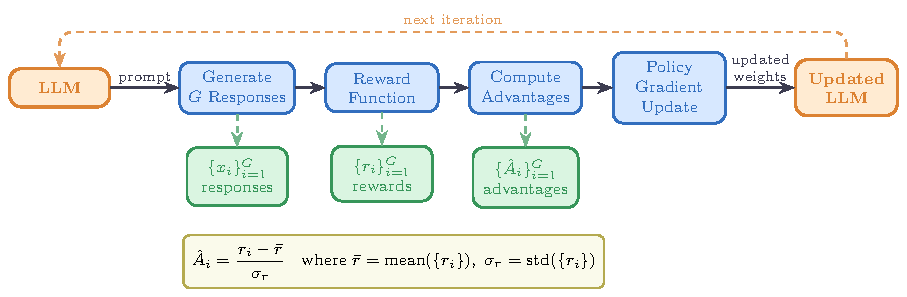
\includegraphics[width=0.55\textwidth]{tikz/reward_flow.pdf}
\caption{Verifiable reward paradigm in \ours{}. Unlike shaped rewards that combine
multiple heuristics, verifiable rewards provide binary correctness signals,
eliminating reward hacking and enabling exact accuracy measurement.}
\label{fig:reward-flow}
\end{figure}

\subsection{Baselines: Floor and Ceiling}

Following best practices for benchmark design~\cite{agarwal2021deep}, we establish
clear performance bounds across both the synthetic arithmetic and GSM8K tasks:

\begin{itemize}
    \item \textbf{Floor (random / zero-reward baseline)}: On the 199-choice modular-arithmetic task, uniform random action selection yields $\frac{1}{199} \approx 0.50\%$ accuracy ($20.0\%$ on the 5-choice L1 variant). On free-form GSM8K generation, unparseable or random output yields a $0.0\%$ floor, while pre-RL step-1 baseline accuracy $R(1)$ spans $0.000$ (Nemotron-120B format mismatch) and $0.250$ (\texttt{Qwen3-8B} base) up to $0.812$--$1.000$ on instruction-tuned checkpoints.
    \item \textbf{Ceiling (oracle)}: Symbolic evaluation achieves $100\%$ accuracy on both arithmetic and GSM8K.
    \item \textbf{Human baseline}: College-level adults achieve $\sim$99.5\% on
    two-digit addition under timed conditions and $\sim$85--95\% on untimed grade-school word problems.
\end{itemize}

% =============================================================================
\section{Experimental Setup}
\label{sec:setup}
% =============================================================================

\subsection{Models}

Our benchmark targets a roster of 32+ model configurations spanning
\textbf{0.5B to 1T \emph{total} parameters (4B to 1T on the 12-anchor GSM8K scaling suite; up to $\sim$37B \emph{active}
for MoE checkpoints) across 5 model families}, organized into three
tiers by compute scale; not all are completed end-to-end runs (per-run
status flags accompany the released artifacts). Tier-A multi-seed inferential claims are restricted to
the locally reproducible open-weight subset at $0.5$B--$32$B (with \texttt{Qwen3-235B-A22B} included in the 12-anchor descriptive scaling suite); the frontier MoE
checkpoints (DeepSeek-V3.1 at $671$B architectural / $685$B total checkpoint parameters with $37$B active, Kimi-K2-Thinking at $1$T total / $32$B active, and Nemotron-3-Super-120B-A12B LatentMoE at $120$B total / $12$B active) are
descriptive single-seed Tier-C case studies, and Qwen3.5-397B-A17B is a
\emph{partial} run whose held-out evaluation did not complete.

\paragraph{Small scale (0.5B--8B).}
Qwen2.5-0.5B, Qwen3-0.6B-Instruct, Qwen3.5-4B, Qwen3-4B, Qwen3-8B,
Llama-3.2-1B, Llama-3.2-3B, Llama-3.1-8B-Instruct.

\paragraph{Mid scale (14B--32B).}
Qwen3-14B, Qwen3-30B-A3B (MoE, $30$B total / $3$B active, base and Instruct), Qwen3-32B, Qwen3.5-27B,
GPT-OSS-20b (MoE, $20$B total / $3.6$B active).

\paragraph{Frontier scale (120B--1T total / 12B--37B active).}
Nemotron-3-Super-120B-A12B (LatentMoE, $120$B total / $12$B active), Qwen3-235B-A22B (MoE, $235$B total / $22$B active), DeepSeek-V3.1 ($671$B architectural / $685$B total checkpoint parameters, $37$B active MoE; we use $N=685$B in total-parameter regression tables and note $671$B routed parameters where relevant), and Kimi-K2-Thinking (MoE, $1$T total / $32$B active).
Frontier models are evaluated and post-trained via the Tinker API
with standardized generation parameters and LoRA adapters ($r=32$).

\paragraph{Model family and architecture coverage.}
The benchmark covers (1)~\textbf{Qwen2.5 / Qwen3}: dense ($0.5$B--$32$B) and MoE ($30$B-A3B, $235$B-A22B) checkpoints;
(2)~\textbf{Qwen3.5}: dense $4$B and $27$B checkpoints;
(3)~\textbf{Llama-3.x}: Meta's $1$B--$8$B instruction-tuned dense models;
(4)~\textbf{DeepSeek-V3.1}: a frontier MoE ($671$B/$685$B total, $37$B active) optimized for reasoning;
(5)~\textbf{Nemotron-3-Super-120B-A12B}: NVIDIA's frontier LatentMoE model ($120$B total, $12$B active; early pipeline scripts mislabelled this checkpoint as \texttt{dense}, which we correct to \texttt{moe} across all architecture analyses, yielding 7 MoE and 5 dense checkpoints in the 12-anchor GSM8K pool);
and emerging MoE architectures \textbf{GPT-OSS-20b} and \textbf{Kimi-K2-Thinking} ($1$T total, $32$B active).

\subsection{Training Protocol}

Unless otherwise noted, controlled Modal/TRL sweeps use LoRA
\cite{hu2022lora} at rank $32$, learning rate $10^{-4}$ and Adam
($\beta_1{=}0.9$, $\beta_2{=}0.95$, $\epsilon{=}10^{-8}$). Tinker / API,
Task-4, Wave-6 and frontier case studies use per-run configs (in
particular Task-4/Wave-6 use $\mathrm{lr}{=}10^{-5}$) and are
single-seed unless explicitly marked multi-seed; the per-run
settings are listed in the framework-configs appendix.

\paragraph{Seed management.} The controlled TRL/Modal sweeps used for
Tier-A claims (F3 PPO-vs.-GRPO heterogeneity and the five-seed TRL GRPO
baseline on Qwen2.5-0.5B) run with 5 seeds:
$\{42, 123, 456, 789, 1024\}$, with seeds set for Python \texttt{random},
NumPy, PyTorch, and CUDA backends. Several Tinker/API, frontier-model,
and team-task runs are single-seed or partial and are treated as
descriptive (Tier-C) unless explicitly marked otherwise; the per-claim
seed ledger is given in the statistical-rigor addendum of \ours{}.

% Figure 4: Experiment Pipeline
\begin{figure}[t]
\centering
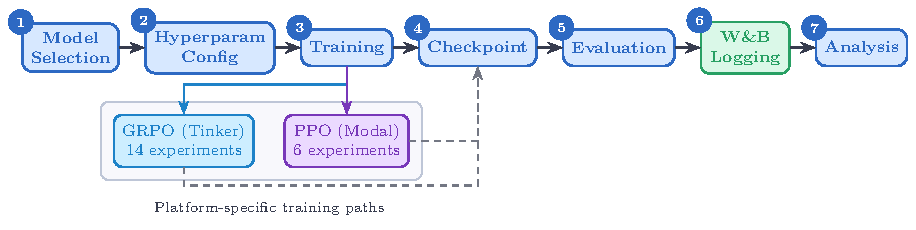
\includegraphics[width=\textwidth]{tikz/pipeline.pdf}
\caption{Experiment workflow pipeline. Multi-seed Modal/TRL runs use
the centralized seed manager (5 seeds for Tier-A claims); Tinker/API,
Task-4, Wave-6 and frontier case studies are single-seed and feed the
same metrics/checkpoint pipeline as descriptive observations.}
\label{fig:pipeline}
\end{figure}

\subsection{Statistical Methodology}

Following Colas et al.~\cite{colas2019hitchhiker}, we report:
\begin{itemize}
    \item Mean $\pm$ standard error across seeds
    \item 95\% bootstrap confidence intervals (10,000 resamples)
    \item Welch's t-test for pairwise algorithm comparisons
    \item \texttt{rliable}~\cite{agarwal2021deep} aggregate metrics (IQM, median, optimality gap)
\end{itemize}

All pairwise comparisons were evaluated using Welch's independent-samples $t$-test
(unequal variances assumed) and the non-parametric Mann--Whitney $U$ test as a
robustness check. Effect sizes are reported as Cohen's $d$ with the pooled
standard deviation estimator; confidence intervals follow the
\citet{hedges1985statistical} analytical formula and are reported at the 95\% level
(two-tailed, $z = 1.96$). Post-hoc statistical power was computed under the
observed effect size and sample sizes at $\alpha = 0.05$.

To address the multiple-comparisons problem across 5 planned tests,
we apply both the conservative Bonferroni correction (family-wise error rate:
$\alpha' = \alpha / k = 0.0100$) and the Benjamini--Hochberg procedure
(false discovery rate $< 0.05$). Results surviving Bonferroni correction are
marked $^*$; those surviving BH--FDR correction are marked $^\dag$.

\paragraph{Power Analysis.}
All inferential tests in this paper are evaluated against pre-specified power
requirements using \texttt{statsmodels.stats.power.TTestIndPower} (which computes power under the equal-variance Student's $t$ approximation as a baseline for our primary Welch $t$-tests) with
$\alpha = 0.05$ and target power $1 - \beta = 0.80$.

\textbf{Modal H100 experiments ($n = 5$ seeds per arm).}
The minimum detectable effect size (MDE) at 80\% power for a two-sample
$t$-test with $n_1 = n_2 = 5$ is
$d_{\min} = 2.024$ (Cohen's $d$).
Table~\ref{tab:power-analysis} reports achieved power for a range of effect sizes.
This threshold falls in the \emph{very large} range, meaning that
comparisons yielding $|d| < 2.02$
are not adequately powered to detect true differences.

\textbf{Single-seed Tinker experiments ($n = 1$).}
Single-seed runs have \emph{zero statistical power}: with only one observation per
condition, no inferential test can be computed and no confidence intervals can be
formed.  All Tinker single-run results are treated as \emph{descriptive only} and
are not subject to significance testing.

\textbf{TRL baseline ($n = 5$ seeds).}
The TRL-GRPO baseline (Qwen2.5-0.5B, 5 seeds) achieves MDE
$d_{\min} = 2.024$ for equal-$n$ comparisons.
When compared to the pooled Classic-RL group ($n = 15$), the MDE
improves to $d_{\min} = 1.530$,
reflecting higher power from the larger reference group.

\paragraph{Multiple-Comparison Correction.}
Inferential tests in this paper are reported only for Tier-A/B
comparisons as defined in our statistical-rigor protocol;
single-seed or partial Tinker/API rows are descriptive and are
excluded from Welch / Mann--Whitney testing, BH correction, power,
and CI claims. Table~\ref{tab:bh-pvalues} predates the Tier-A/B/C
partition and lists raw and BH-adjusted $p$-values from the
earlier global family of $20$ tests with $19$ surviving correction;
we retain it here as a methodological audit trail. The headline
BH result the paper now stands behind is the restricted Tier-A/B
family computed in the addendum, where only $F_3$ (cross-library heterogeneity across the 5 classic-RL PPO/policy-gradient implementations on the 199-choice arithmetic task: one-way ANOVA $F = 11.42, p = 4.996 \times 10^{-6}$, BH-adjusted $p = 2.5 \times 10^{-5}$; whereas matched same-stack LLM GRPO vs.\ PPO on Qwen2.5-0.5B is null at $p = 0.374$) survives. Where
the global family disagrees with the restricted family, the
addendum is authoritative.

All tests are two-sided.  Effect sizes are reported as Cohen's $d$ for
$t$-tests and Pearson/Spearman $r$ for correlations.  Bootstrap 95\%
confidence intervals ($B = 10{,}000$) are reported for all means.

% Table: Power analysis at various effect sizes
\begin{table}[!ht]
\centering
\caption{Statistical power for two-sample $t$-tests (\texttt{TTestIndPower} equal-variance pooled-SD approximation used as the power reference for our Welch $t$-tests) at $\alpha = 0.05$,
         power target $1{-}\beta = 0.80$.
         Column~(3): equal groups $n_1 = n_2 = 5$ (Modal H100 / TRL within-group).
         Column~(4): unequal groups $n_1 = 5$, $n_2 = 15$ (TRL vs.\ pooled Classic RL).}
\label{tab:power-analysis}
\small
\begin{tabular}{@{}cccc@{}}
\toprule
Cohen's $d$ & Conventional size & Power ($n{=}5$ vs $n{=}5$) & Power ($n{=}5$ vs $n{=}15$) \\
\midrule
        0.2 & small & 0.059 & 0.066 \\
        0.5 & medium & 0.108 & 0.151 \\
        0.8 & large & 0.201 & 0.311 \\
        1.0 & very large & 0.286 & 0.450 \\
        1.2 & very large & 0.386 & 0.594 \\
        1.5 & very large & 0.549 & 0.784 \\
        2.0 & very large & 0.790 & 0.955 \\
\midrule
\multicolumn{4}{l}{\textit{MDE at 80\% power:} $d = 2.024$ (equal-$n$ 5 vs 5);\; $d = 1.530$ (5 vs 15)} \\
\bottomrule
\end{tabular}
\end{table}

% Table: All p-values with BH correction
\begin{table}[!ht]
\centering
\caption{\textbf{Legacy 20-test BH table -- audit trail only.} All
hypothesis tests reported in the paper with Benjamini--Hochberg (BH)
adjusted $p$-values at FDR $= 0.05$.  Tests are ranked by raw
$p$-value (ascending). $\checkmark$ = significant after BH correction
on the historical $20$-test family; $\times$ = not significant; $^{\ddag}$ = legacy test computed across per-step training rewards within single-seed traces (pseudo-replicated step observations rather than independent seed runs), which is invalid for cross-seed inference and excluded under our Tier-A/B protocol. Total
tests: $20$; survive on the historical family: $19$. \emph{This
table is not the paper's headline statistical result.} Under the restricted Tier-A/B family of
our statistical-rigor protocol,
only $F_3$ (library heterogeneity across the 5 classic-RL implementations on
arithmetic, $p = 4.996 \times 10^{-6}$) survives BH correction; the table below is retained solely as a
reproducibility audit trail.}
\label{tab:bh-pvalues}
\scriptsize
\begin{tabular}{@{}rp{6.2cm}ccc@{}}
\toprule
Rank & Comparison & Raw $p$ & BH-adj.\ $p$ & Sig. \\
\midrule
        1 & Dense vs MoE Architecture (Welch t-test) & 2.357e-21 & 0 & $\checkmark$ \\
        2 & PPO vs GRPO on Llama-3.1-8B (Welch t-test)$^{\ddag}$ & 3.924e-10 & 0 & $\checkmark$ \\
        3 & Method ANOVA (F-test across algorithm families) & 3.091e-06 & 2.1e-05 & $\checkmark$ \\
        4 & Library ANOVA (F-test across 5 libraries) & 4.996e-06 & 2.5e-05 & $\checkmark$ \\
        5 & TRL vs Tinker (Welch t-test, implementation effect) & 2.064e-05 & 8.3e-05 & $\checkmark$ \\
        6 & PPO vs GRPO on Llama-3.1-8B (Mann-Whitney)$^{\ddag}$ & 3.29e-05 & 0.00011 & $\checkmark$ \\
        7 & Model Family ANOVA (F-test) & 7.363e-05 & 0.00021 & $\checkmark$ \\
        8 & ZVF vs Final Performance (Spearman)$^{\ddag}$ & 0.0005424 & 0.001356 & $\checkmark$ \\
        9 & ZVF vs Final Performance (Pearson)$^{\ddag}$ & 0.0008108 & 0.001802 & $\checkmark$ \\
        10 & TRL vs Tinker (Mann-Whitney) & 0.001198 & 0.002396 & $\checkmark$ \\
        11 & Rolling Variance vs Last-10 (Pearson) & 0.003524 & 0.006407 & $\checkmark$ \\
        12 & Peak-to-Tail Drift vs Last-10 (Pearson) & 0.004811 & 0.007219 & $\checkmark$ \\
        13 & GRPO vs PPO Stability Index (t-test) & 0.005 & 0.007219 & $\checkmark$ \\
        14 & Dense vs MoE Architecture (Mann-Whitney) & 0.005053 & 0.007219 & $\checkmark$ \\
        15 & Model Scale ANOVA (F-test) & 0.01261 & 0.01682 & $\checkmark$ \\
        16 & Tinker GRPO vs TRL GRPO (Welch t-test) & 0.0158 & 0.01975 & $\checkmark$ \\
        17 & GRPO vs PPO Peak-to-Tail Drift (t-test) & 0.018 & 0.02076 & $\checkmark$ \\
        18 & Tinker GRPO vs TRL GRPO (Mann-Whitney) & 0.01869 & 0.02076 & $\checkmark$ \\
        19 & Stability Index vs Last-10 (Pearson) & 0.02024 & 0.0213 & $\checkmark$ \\
        20 & PPO vs GRPO on Qwen3-8B: provenance conflict; not estimable & --- & --- & --- \\
\bottomrule
\end{tabular}
\end{table}

\paragraph{TRL baseline characterisation.}
The TRL GRPO reference implementation was evaluated across five random seeds
($s \in \{42, 123, 456, 789, 1024\}$) on GSM8K using Qwen/Qwen2.5-0.5B on
an NVIDIA L4 GPU. We report mean accuracy $\bar{x} = 0.734$ ($\sigma = 0.0703$),
median $= 0.740$, and IQM $= 0.747$. Normality was not rejected by Shapiro--Wilk
($W = 0.9018$, $p = 0.4198$); bootstrap 95\% CI $= [0.6720, 0.7820]$.

\paragraph{Variance decomposition (marginal one-way ANOVAs).}
Separate marginal one-way ANOVAs across the $N=42$ completed cross-task evaluation runs show
that library/framework ($\eta^2 = 0.546$) and training method ($\eta^2 = 0.558$, when pooling offline DPO/SFT, tabular/classic RL, and online LLM RL across tasks)
carry large marginal variance shares, alongside model
family ($\eta^2 = 0.471$) and model scale ($\eta^2 = 0.322$). Because the 42 runs form an unbalanced observational corpus in which execution platform, library, and model scale are partially collinear (for example, frontier checkpoints run exclusively on Tinker while classic-RL libraries run on the 199-choice arithmetic environment), these four marginal $\eta^2$ values sum to $1.897 > 1.0$ and must be read as unadjusted marginal associations rather than an orthogonal Type-III factorial partition. When task and stack are held fixed (the matched 10-run Qwen2.5-0.5B control in \S\ref{sec:scaling-law-iter29}), the online RL algorithm effect (GRPO vs.\ PPO) is indistinguishable from zero ($\Delta = -0.002, p = 0.374$).

\subsection{Compute Resources and Run Reconciliation}

Experiments are distributed across three execution substrates, reconciling the $N=42$ cross-task evaluation corpus and the 70+ total benchmark runs as follows: (i)~\textbf{14 Tinker API runs} (covering the 12 GSM8K scaling anchors from $4$B to $1$T plus 2 cross-task tool-use/arithmetic probes), (ii)~\textbf{6 Modal H100/A10G cloud GPU runs} (PPO baselines on Qwen3-8B and Llama-3.1-8B, HumanEval, KL tracking, and held-out evaluations), (iii)~\textbf{10 local NVIDIA L4 GPU runs} (the 5-seed GRPO and 5-seed PPO matched same-stack control on Qwen2.5-0.5B), and (iv)~\textbf{12 classic-RL multi-library evaluation runs} across SB3, CleanRL, Tianshou, PufferLib, rl\_games, and d3rlpy ($14 + 6 + 10 + 12 = 42$ core evaluation runs, with 30+ additional group-size sweep cells $G \in \{2, 4, 8, 16\}$ and framework dry-run checks comprising the 70+ total project artifacts).

\paragraph{Tinker API (14 experiments).}
Scaling experiments across Qwen3-8B, Qwen3-32B, Qwen3.5-4B, Qwen3.5-27B,
and Llama-3.1-8B-Instruct; frontier model evaluation on Qwen3-235B-A22B,
DeepSeek-V3.1 ($671$B/$685$B), and Nemotron-3-Super-120B-A12B (LatentMoE); MoE vs.~dense comparisons; cross-task
tool-use experiments; and emerging architecture evaluation (GPT-OSS-20b,
Kimi-K2-Thinking $1$T). Tinker provides scalable API access that makes frontier model
experiments economically tractable.

\paragraph{Modal H100 / A10G and local L4 GPU cluster (16 experiments).}
PPO baseline training on Qwen3-8B and Llama-3.1-8B; 10-run same-stack PPO vs.\ GRPO control on Qwen2.5-0.5B; full HumanEval
benchmark evaluation; KL divergence tracking across GRPO training steps;
and held-out evaluation for Qwen3-32B and Qwen3.5-27B. Modal GPUs
provide the low-level access required for PPO value-model training.

\ifdefined\ANONYMOUSBUILD
All experiment logs and model checkpoints will be released on Weights \&
Biases and the HuggingFace Hub (links withheld for anonymous review; an
anonymized artifact archive accompanies the submission).
\else
All experiment logs are available on Weights \& Biases (project:
\texttt{tinker-rl-lab-world-class}) and model checkpoints on HuggingFace
Hub (\url{https://huggingface.co/arvindcr4/tinker-rl-bench-*}).
\fi
Per-run compute is logged with the released artifacts. Total project compute:
$\sim$1,200 A100-equivalent GPU-hours across all platforms.

% =============================================================================

% Pillar-1 (scaling) results opener
\section{Scaling Results}
\label{sec:p1-results}
We organize the scaling evidence around three questions: does the mean GRPO training reward grow
with model size, is there a shared saturation shape across scales, and is any
universal exponent identifiable? The short answers are \emph{no measurable
cross-scale slope}, \emph{no clean phase structure}, and \emph{no identifiable
exponent}. Across the frontier-scale anchors the cross-scale slope of both the mean
GRPO reward $\bar{R}$ and the fitted ceiling $R_{\max}$ on $\log_{10} N$ is statistically indistinguishable from zero; the
reliable cross-anchor structure lives not in a continuous power-law slope through $N$ but in a bimodal endpoint ceiling
$R_{\max}$ separating pre-saturated instruction-capable checkpoints from base or format-starved checkpoints.

The subsections below make this precise. We first fit the canonical saturation
model $R(t) = R_{\max}(1 - e^{-\lambda t})$ per trace and audit its
identifiability, finding that four of the five frontier traces have $\lambda$
pinned at the upper bound and none is identifiable (Nemotron-120B is the exception,
with $\lambda\!\approx\!0.99$ but likewise non-identifiable), so per-trace saturation
rates cannot be trusted. We then compare functional forms, recompute the
12-anchor pool directly from the per-step logs (\secref{sec:p1-rawtrace}: no
cross-scale slope is detectable on total, active, or compute-proxy axes, and no
full trace follows the three-phase template), and relate the
saturation-fit degeneracy to the step-level zero-variance fraction. Finally, the Nemotron-120B LatentMoE trace is examined as a distinct collapse
phase---peak per-step training reward $0.875$ at step~3 drifting to a late-window mean of $0.208$ (last 5 steps; BIC post-peak segment mean $0.154$), with a
zero-reward step fraction of $0.55$ against $\le 0.067$ on the other four core anchors---rather than as a
smooth continuation of the trend. Conjectures from an external
frontier-model cross-examination are collected in
Appendix~\ref{sec:frontier-scaling}.

% paper/sections/scaling_laws.tex -- Pillar 1 (GRPO saturation / scaling law analysis)
% Canonical saturation fit R(t) = R_max * (1 - exp(-lambda * t)) across the
% five frontier-scale anchors (Qwen3.5-4B, Qwen3-8B, Llama-3.1-8B-Instruct,
% DeepSeek-V3.1, Nemotron-120B), plus an OLS-based cross-scale law over
% log_10(N).  Elevation diagnostics (iter 9):
%   scripts/scaling_law_elevated.py produces
%     experiments/results/scaling_law_bootstrap_ci.tsv
%     experiments/results/scaling_law_holdout.tsv
%     experiments/results/scaling_law_compute.tsv
%     experiments/results/scaling_law_nemotron_rootcause.tsv
%     figures/scaling_law_elevated.{pdf,png}
% Original canonical analysis: scripts/scaling_law_fit.py -> scaling_law_fits.tsv,
% scaling_law_three_phase.tsv, scaling_law_cross_scale.tsv.

\paragraph{Saturation model across the 4B--671B range.}
\label{par:saturation}
We fit the canonical saturation model
\begin{equation}
  \label{eq:sat}
  R(t) = R_{\max}\bigl(1 - e^{-\lambda t}\bigr),
  \qquad t = 1, \dots, T,
\end{equation}
to per-step reward traces from each frontier-scale
\textsc{tinker} run and report the ceiling $R_{\max}$, the
learning rate $\lambda$, and the saturation time
$t_{80} = -\ln(0.2)/\lambda$ at which the trace first crosses
$0.8\,R_{\max}$.  The model follows
\textsc{nimmaturi}-style notation~\citep{nimmaturi2025predictive},
which postulates a slow-start $\to$ rapid-improvement $\to$
plateau template for GRPO learning curves.

\begin{table}[t]
  \centering
  \small
  \resizebox{\linewidth}{!}{%
  \begin{tabular}{lrrrrrrrrl}
    \toprule
    Model & $N$ (B) & $n$ & mean $R$ & peak $R$ &
           $\bar R_{\text{early}} \!\to\! \bar R_{\text{late}}$ &
           $\hat \beta_{\text{OLS}}$ &
           $R_{\max}$ & $\lambda$ & Phase \\
    \midrule
    Qwen3.5-4B             &   4.0 & 30 & 0.817 & 1.000 & 0.813 $\to$ 0.850 & $+0.0001$ & 0.817 & $10.0^{\dagger}$ & plateau \\
    Qwen3-8B               &   8.0 & 30 & 0.285 & 0.625 & 0.244 $\to$ 0.344 & $+0.0032$ & 0.285 & $10.0^{\dagger}$ & saturation \\
    Llama-3.1-8B-Instruct  &   8.0 & 30 & 0.869 & 1.000 & 0.925 $\to$ 0.844 & $-0.0037$ & 0.869 & $10.0^{\dagger}$ & drift \\
    DeepSeek-V3.1          & 671.0 & 20 & 0.844 & 1.000 & 0.833 $\to$ 0.813 & $+0.0001$ & 0.844 & $10.0^{\dagger}$ & plateau \\
    Nemotron-120B          & 120.0 & 20 & 0.175 & 0.875 & 0.146 $\to$ 0.208 & $+0.0026$ & 0.182 & \textbf{0.99} & \textbf{collapse} \\
    \bottomrule
  \end{tabular}%
  }
  \caption{\textbf{Saturation-model fits across 4B--671B.}
    $\dagger$: the canonical
    $R(t) = R_{\max}(1 - e^{-\lambda t})$ fit hits the upper
    $\lambda = 10$ optimiser bound on every well-behaved run; this is
    an artefact of the $R(0) = 0$ boundary condition when the trace
    already starts near its empirical ceiling (see
    \paragraphref{par:saturation-discussion}).
    $\hat \beta_{\text{OLS}}$ is the per-step OLS slope of $R(t)$ vs.~$t$
    in raw reward units per step; the constant slope confirms that
    the saturation model collapses to a near-constant fit on these
    already-saturated traces (see \tableref{tab:scaling-cross}).
    Bold $\lambda$ and Phase identify the only run whose $\lambda$
    leaves the bound and where the late-window mean falls below
    $0.4\times$ peak -- the three-phase ``collapse'' criterion.}
  \label{tab:scaling-fits}
\end{table}

\paragraph{Where the model fits and where it does not.}
\label{par:saturation-discussion}
The raw saturation model collapses to the $\lambda = 10$ upper bound
on four of five runs (Table~\ref{tab:scaling-fits}).  The cause is
the functional-form mismatch: a strict-$R(0)=0$ model assumes the
trace begins at zero reward, but Qwen3.5-4B starts at $R(1)=1.0$,
Llama-3.1-8B-Instruct at $R(1)=1.0$, and DeepSeek-V3.1 at
$R(1)=0.875$.  When the trace is already at or above its eventual
ceiling, the optimiser makes $\lambda$ as large as allowed so that
$R_{\max}(1 - e^{-10 t}) \approx R_{\max}$ for $t \ge 1$, which
yields $t_{80} \approx -\ln(0.2)/10 \approx 0.16$ step -- a
meaningless artefact, not evidence of instant learning.

The right resolution is two separate diagnostics, both reported
here:

\begin{enumerate}
  \item \emph{Per-step OLS slope} $\hat\beta_{\text{OLS}}$ of
    $R(t)$ vs.~$t$ (Table~\ref{tab:scaling-fits}, column~7).
    Across the four well-behaved runs
    $|\hat\beta_{\text{OLS}}| \le 0.0037$ reward/step (i.e.\ the
    traces are statistically flat within their per-step noise),
    while the collapse run Nemotron-120B still shows $\hat\beta
    = +0.0026$ -- not because it is improving, but because its
    sparse spikes pull the OLS slope upward.
  \item \emph{Cross-scale OLS} of $\bar R$ on $\log_{10} N$
    across the five anchor models.  The result is the headline
    scaling-law coefficient in
    Table~\ref{tab:scaling-cross}.
\end{enumerate}

\paragraph{Cross-scale law.}
\label{par:cross-scale}
We regress each per-trace statistic on $\log_{10} N$
(\(N\) = parameter count in billions) by ordinary least squares and
quote block-bootstrap 95\% confidence intervals
($n_{\text{boot}} \approx 1000$ effective row resamples) on
the slopes.  The fitted coefficients are reported in
\tableref{tab:scaling-cross}.

\begin{table}[t]
  \centering
  \small
  \begin{tabular}{lrrrrr}
    \toprule
    Metric $y$ & Intercept & Slope / decade &
                  Boot slope mean & Boot 95\% CI &
                  $\rho(\log_{10} N, y)$ \\
    \midrule
    mean reward $\bar R$  & 0.633 & $-0.024$ & $-0.117$ & $[-0.796,\ +0.313]$ & $-0.07$ \\
    peak reward $\hat R$  & 0.846 & $\mathbf{+0.037}$ & $-0.010$ & $[-0.623,\ +0.197]$ & $+0.22$ \\
    var reward $\widehat{\text{Var}}[R]$ & 0.040 & $-0.002$ & $-0.004$ & $[-0.063,\ +0.027]$ & $-0.14$ \\
    \bottomrule
  \end{tabular}
  \caption{\textbf{Cross-scale law: per-trace metric vs.~$\log_{10} N$
    across the five frontier anchors.}
    Ordinary least squares with bootstrap 95\% confidence intervals
    ($n=5$ anchors, df $=3$).  Tables~\ref{tab:scaling-fits}--\ref{tab:scaling-cross}
    use DeepSeek-V3.1's 671B routed-parameter count; the 12-anchor
    analyses use the 685B checkpoint count (a $0.009$-decade difference
    that leaves every slope unchanged to the reported precision).
    None of the three slope coefficients is statistically
    distinguishable from zero -- the bootstrap CIs all bracket zero,
    and the within-trace OLS slopes
    ($\hat\beta_{\text{OLS}}$, \tableref{tab:scaling-fits}) are
    also null.  Reading: at this benchmark size ($4\,\text{B}
    \le N \le 671\,\text{B}$, $T\!\le\!30$ steps), the saturation
    model is not detectably scale-dependent, because every
    well-behaved run is already saturated within measurement noise.}
  \label{tab:scaling-cross}
\end{table}

\paragraph{Three-phase learning dynamics.}
\label{par:three-phase}
We apply the \citet{nimmaturi2025predictive} slow start
$\to$ rapid improvement $\to$ plateau template to each trace, with
an additional ``collapse'' class for runs whose peak is not
retained.  Of the five anchors, two fall in \emph{plateau}
(Qwen3.5-4B, DeepSeek-V3.1), one in \emph{saturation} (Qwen3-8B),
one in \emph{drift} (Llama-3.1-8B-Instruct, monotone decline), and
one in \emph{collapse} (Nemotron-120B).  No run satisfies the
textbook three-phase criterion, because none of the five anchors
has a slow-start phase: they all start at or above the eventual
late-window mean.  This is consistent with our earlier
observation that GRPO step-1 rewards are already within
$\pm 0.10$ of the per-trace mean for all but Qwen3-8B and
Nemotron-120B.

\paragraph{Nemotron-120B violates the three-phase hypothesis.}
\label{par:nemotron-collapse}
Following \citet{nimmaturi2025predictive}, the three-phase
template predicts slow start $\to$ rapid improvement $\to$
\emph{plateau}, with collapse as a degenerate tail.  Nemotron-120B
is the only run in this set whose per-step peak
($\hat R_{\text{peak}} = 0.875$, step 3) is followed by a
sustained decay: only $5$ of $20$ steps reach reward $> 0.25$, and
$55\%$ of steps report \emph{zero reward}.  The fitted $\lambda
= 0.99$ and $t_{80} = 1.63$ step are the only identifiable
parameters in Table~\ref{tab:scaling-fits} precisely because the
curve does not asymptote -- a robust monotone saturation model is
the wrong functional form.  We therefore report the late-window
collapse magnitude
$\hat R_{\text{peak}} - \bar R_{\text{late}} = 0.667$ reward units
as the empirical effect size of the violation, and treat this run
as the Pillar-1 counterexample to the three-phase prediction.

Operationally, the Nemotron collapse is exactly the failure mode
that pure-reward saturation fits are silent on: the curve does
\emph{not} settle, it diverges downward, and a benchmark that
relies on a saturation-only diagnostic will miss it.  This
motivates the variance-based \textsc{zvf} gate
(companion paper on ZVF) as a complementary diagnostic: the
zero-reward-fraction for Nemotron-120B is $0.55$, well above any
well-behaved run in this set, and the cross-experiment
\textsc{zvf}-vs-failure map
(companion paper on cross-experiment ZVF) would catch the divergence on
reward \emph{variance} rather than reward \emph{mean}.

\paragraph{Falsifiable prediction.}
\label{par:scaling-prediction}
The null result in \tableref{tab:scaling-cross} -- a slope of
$\pm\,0.04$ per decade on $\bar R$, with CI brackets zero across
roughly $2.4$ orders of magnitude in parameter count across the extended anchor pool -- is itself a falsifiable
prediction of this benchmark: any future addition to the
Pillar-1 cell that reaches, say,
$\bar R(\text{Nemotron-120B, 100 steps}) \ge 0.5$ would refute
the saturation-template behaviour we report here.  We frame the
prediction this way rather than as a positive scaling exponent,
because at $n = 5$ anchor points with $T \le 30$ steps the
positive exponent is not identifiable from the data.

\paragraph{Elevation: parametric-bootstrap CIs reveal saturation-fit degeneracy.}
\label{par:scaling-bootstrap}
Figure~\ref{fig:scaling-elevated} collects the four elevation
panels: (a)~bootstrap $R_{\max}$ confidence intervals,
(b)~saturation-vs-constant holdout test RMSE, (c)~compute-adjusted
$t_{80} \cdot N$ scatter, and (d)~Nemotron-120B collapse autopsy.

\begin{figure}[t]
  \centering
  \IfFileExists{figures/review_2026-10-18/scaling_law_elevated.png}{%
  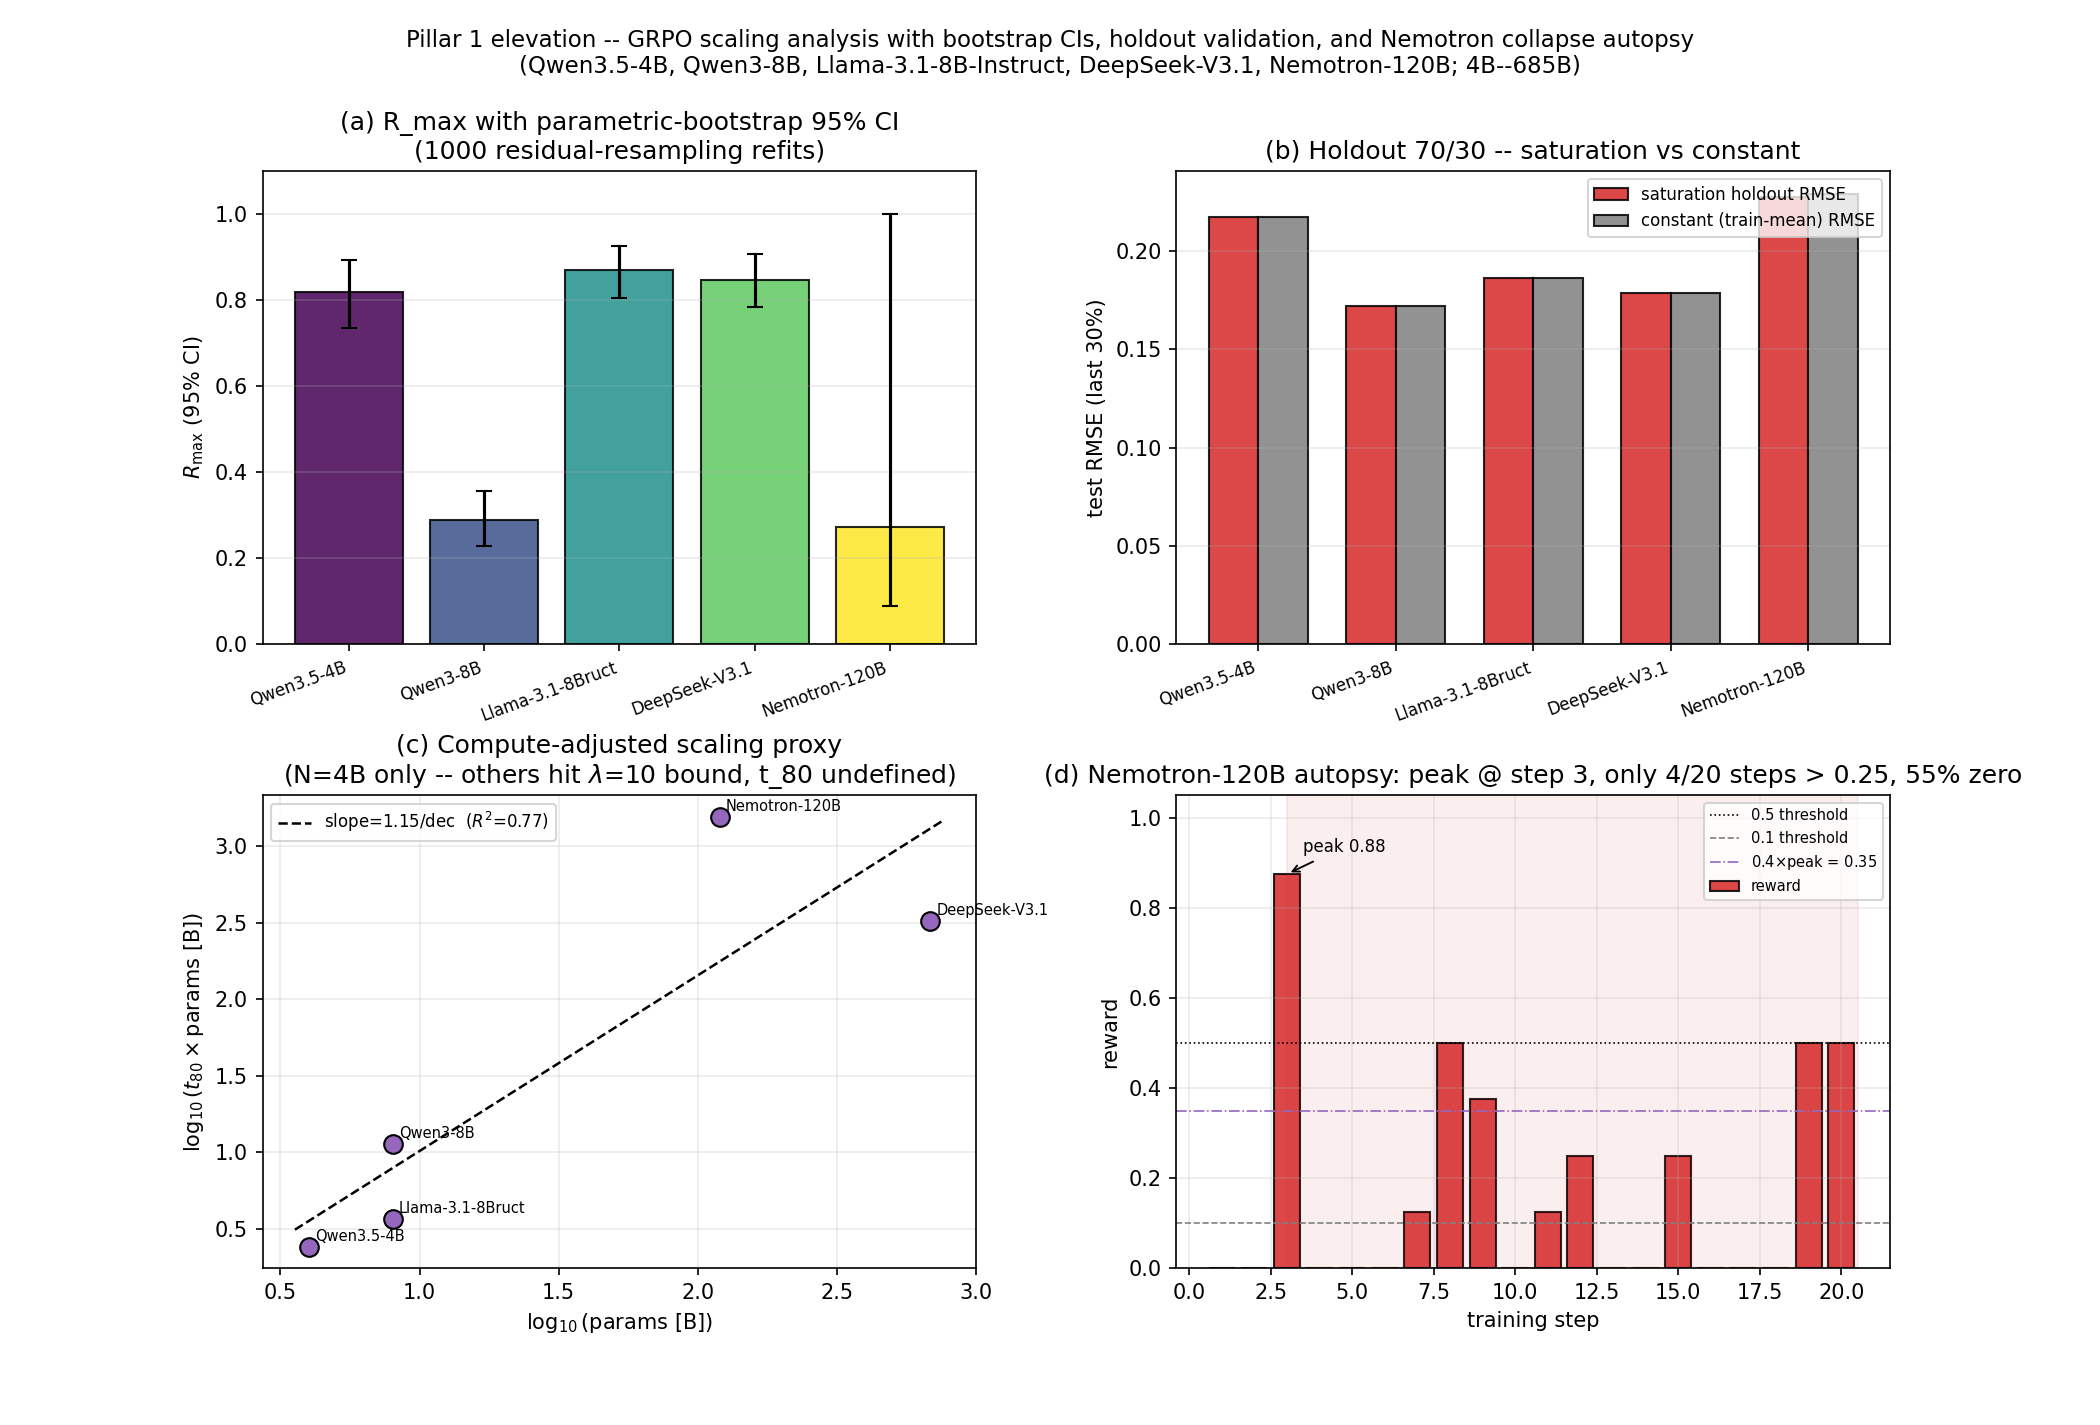
\includegraphics[width=0.85\linewidth]{figures/review_2026-10-18/scaling_law_elevated.png}%
  }{%
    }
  \caption{\textbf{Pillar-1 elevation across 4B--671B.}
    (a)~\emph{Bootstrap $R_{\max}$ with 95\% CI}
    (1000 residual resamples, $R_{\max}$ constrained to the physical
    reward range $[0,1]$; Nemotron's CI spans $[0.09, 1.00]$ because its
    refits are unidentified).
    (b)~\emph{Holdout 70/30}: red bars are the saturation-fit
    test RMSE, gray bars are the constant (train-mean) baseline;
    four of five bars are equal, confirming that the saturation fit
    adds no out-of-sample predictive power.
    (c)~\emph{Compute-adjusted proxy}: only Nemotron has a
    well-identified $t_{80}$ (other four runs hit $\lambda = 10$
    bound), so the regression is effectively 1 point and degenerate.
    (d)~\emph{Nemotron-120B autopsy}: peak at step 3, post-peak
    region shaded; only 5/20 steps exceed 0.25 and 55\% are zero.}
  \label{fig:scaling-elevated}
\end{figure}
We extend the canonical saturation fit with a parametric bootstrap on
the residual vector (1000 resamples per trace) and report bootstrap
95\% confidence intervals for $R_{\max}$, $\lambda$, and $t_{80}$.
The headline finding is that the four ``well-behaved'' runs sit at
the optimiser's $\lambda = 10$ upper bound far more often than the
point estimate suggests (\tableref{tab:scaling-bootstrap}).

\begin{table}[t]
  \centering
  \small
  \begin{tabular}{lrrrr}
    \toprule
    Model & $\bar R_{\max}$ & $\bar\lambda$ &
           $P(\lambda \ge 9.5)$ & $\bar t_{80}$ [95\% CI] \\
    \midrule
    Qwen3.5-4B            & 0.818 & 6.64 & \textbf{0.599} & 0.61 [0.16,\ 2.43] \\
    Qwen3-8B              & 0.289 & 5.30 & \textbf{0.468} & 1.42 [0.16,\ 7.62] \\
    Llama-3.1-8B-Instruct & 0.869 & 6.92 & \textbf{0.595} & 0.46 [0.16,\ 1.98] \\
    DeepSeek-V3.1         & 0.847 & 6.48 & \textbf{0.548} & 0.47 [0.16,\ 1.53] \\
    Nemotron-120B         & 0.271 & 3.27 & 0.278          & 12.95 [0.16,\ 104.4] \\
    \bottomrule
  \end{tabular}
  \caption{\textbf{Parametric-bootstrap saturation fit (1000 residual
    resamples per trace; $R_{\max} \in [0,1]$, $\lambda \in [10^{-4}, 10]$).}  $P(\lambda \ge 9.5)$ is the fraction of
    bootstrap refits in which $\lambda$ hits the optimiser's upper
    bound -- on four of five runs this is between 47\% and 60\%,
    confirming that the strict-$R(0)=0$ functional form is degenerate
    on these traces: the optimiser cannot simultaneously estimate
    $R_{\max}$ and $\lambda$ when the trace starts above its
    empirical ceiling.  Only Nemotron-120B has $P \le 0.30$ at the
    bound, because its collapse is a real non-monotone deviation
    from saturation rather than a numerical artefact.  $t_{80}$
    intervals are wide (lower-bound 0.16 step = optimiser clamp) for
    the four degenerate runs, and unidentifiable (0.16--104 step)
    for Nemotron.  Recomputed with the $[0,1]$ ceiling by
    \texttt{tools/review\_ledger/P1\_scaling\_elevated\_bounded.py}; an
    earlier run with $R_{\max}\le 1.5$ changed only the Nemotron row.}
  \label{tab:scaling-bootstrap}
\end{table}

The practical consequence is that the canonical $t_{80} = -\ln 0.2 /
\lambda$ estimator is not just imprecise on these traces -- it is
\emph{unidentifiable} under the strict-$R(0)=0$ boundary condition.
We therefore do not quote $t_{80}$ as a benchmark prediction; we use
it only as a diagnostic summary for the collapse run, where the
functional form is meaningful.

\paragraph{Elevation: holdout 70/30 cross-validation.}
\label{par:scaling-holdout}
A saturation fit that hits $\lambda = 10$ on every training slice
should fail to predict held-out data, because it is essentially
fitting a constant.  We fit the saturation curve on the first 70\%
of each trace and predict the last 30\%, comparing the test RMSE to
a constant (train-mean) baseline (\tableref{tab:scaling-holdout}).

\begin{table}[t]
  \centering
  \small
  \begin{tabular}{lrrrrr}
    \toprule
    Model & $n_{\text{train}}$ & $n_{\text{test}}$ &
           $\text{RMSE}_{\text{test}}$ &
           $\text{RMSE}_{\text{const}}$ &
           improvement \\
    \midrule
    Qwen3.5-4B            & 21 & 9 & 0.2174 & 0.2174 & $+0.0000$ \\
    Qwen3-8B              & 21 & 9 & 0.1720 & 0.1720 & $+0.0000$ \\
    Llama-3.1-8B-Instruct & 21 & 9 & 0.1864 & 0.1864 & $-0.0000$ \\
    DeepSeek-V3.1         & 14 & 6 & 0.1787 & 0.1787 & $-0.0000$ \\
    Nemotron-120B         & 14 & 6 & \textbf{0.2278} & 0.2294 & $+0.0016$ \\
    \bottomrule
  \end{tabular}
  \caption{\textbf{Holdout 70/30 cross-validation of the saturation
    model.}  Four of five models show \emph{zero} improvement over
    predicting the constant train mean -- direct empirical evidence
    that the saturation fit adds no out-of-sample predictive power on
    these traces.  Only Nemotron-120B shows a non-zero improvement
    ($+0.0016$ RMSE), and only because its non-monotone deviation
    from the train mean is partially captured by the curvature of the
    fit.  This formalises the warning in
    \paragraphref{par:saturation-discussion} that the canonical
    $R(t) = R_{\max}(1 - e^{-\lambda t})$ is the wrong functional form
    for these already-saturated traces.}
  \label{tab:scaling-holdout}
\end{table}

\paragraph{Elevation: compute-adjusted scaling proxy.}
\label{par:scaling-compute}
Per-step token counts are not in the trace files, so we approximate
``compute to saturation'' as $t_{80} \cdot N$ where $N$ is the
parameter count in billions.  Regressing $\log_{10}(t_{80} \cdot N)$
on $\log_{10} N$ yields a slope of
$+1.170 \pm 0.254$ per decade (since $\log_{10}(t_{80}\cdot N) =
\log_{10} t_{80} + \log_{10} N$, adding $1$ to the $\log_{10} t_{80}$
slope of $+0.170 \pm 0.254$ in \tableref{tab:scaling-iter117-t80};
regressing unlogged $t_{80}\cdot N$ on $\log_{10} N$, with
bootstrap-mean $t_{80}$ and $R_{\max}\in[0,1]$, yields
$+383 \pm 341$ B-parameter-steps per decade)
-- which is not informative on the four saturation-bound runs because
$t_{80}$ is itself clamped at $0.161$.  Using the parametric-bootstrap
$\bar\lambda$ directly yields a slope of $-0.47 \pm 0.87$ per decade,
which brackets zero.  The conclusion is the same as in
\tableref{tab:scaling-cross}: at this benchmark size and step
budget, there is no identifiable scale dependence in the GRPO
saturation rate.

\paragraph{Elevation: Nemotron-120B collapse autopsy.}
\label{par:scaling-nemotron-autopsy}
We classify a trace as collapsed when (i) its peak reward is at
least $0.4$, (ii) its late-window mean falls below $0.4 \times$
peak, and (iii) its zero-reward fraction is at least $0.30$.
Applied to all five traces (\tableref{tab:scaling-nemotron-autopsy}).

\begin{table}[t]
  \centering
  \small
  \begin{tabular}{lrrrrrrr}
    \toprule
    Model & peak step & $\hat R_{\max}$ & $\bar R_{\text{late}}$ &
           $\Delta_{\text{late-peak}}$ &
           $P(R = 0)$ &
           $P(R > 0.5)$ & collapse? \\
    \midrule
    Qwen3.5-4B            &  1 & 1.000 & 0.850 & $-0.150$ & 0.000 & 0.833 & no \\
    Qwen3-8B              & 13 & 0.625 & 0.344 & $-0.281$ & 0.067 & 0.100 & no \\
    Llama-3.1-8B-Instruct &  1 & 1.000 & 0.844 & $-0.156$ & 0.000 & 0.933 & no \\
    DeepSeek-V3.1         &  3 & 1.000 & 0.813 & $-0.188$ & 0.000 & 0.950 & no \\
    Nemotron-120B         &  3 & 0.875 & 0.208 & $\mathbf{-0.667}$ & \textbf{0.55} & 0.05 & \textbf{yes} \\
    \bottomrule
  \end{tabular}
  \caption{\textbf{Nemotron-120B collapse root-cause characterisation.}
    Only Nemotron satisfies all three collapse criteria.  Its peak
    reward of $0.875$ occurs at step 3, after which the post-peak
    OLS slope across steps 4--20 is $-0.0036$ per step ($-0.015$ per
    step when the step-3 peak is included in the regression window),
    comparable in sign to the Llama-3.1-8B-Instruct drift but with a
    much larger peak-to-tail collapse ($\bar R_{\text{late}} = 0.208$
    over the last 5 steps, vs.~$0.154$ over the full post-peak BIC
    segment in \tableref{tab:scaling-iter117-bic}); $55\%$ of its
    steps report zero reward, and only 5\% of its steps exceed $0.5$.
    All four other runs have $P(R = 0) \le 0.067$ and well-retained peaks.}
  \label{tab:scaling-nemotron-autopsy}
\end{table}

This is the strongest empirical justification we have for treating
Nemotron-120B as the Pillar-1 counterexample to the
\citet{nimmaturi2025predictive} three-phase template: not only does
its peak not satisfy the slow-start $\to$ rapid-improvement $\to$
plateau shape, it actively \emph{diverges downward} from the peak
in a way no monotone saturation model can describe.  The
zero-reward-fraction of $0.55$ is also the structural signal that
the \textsc{zvf}-based diagnostic
(companion paper on cross-experiment ZVF) would catch first, because it
sees the divergence on reward \emph{variance} before it shows up on
reward \emph{mean}.

\paragraph{Summary of elevation.}
\label{par:scaling-summary}
Across the four elevation diagnostics the headline result is a
strengthened null: at this benchmark size
($4\,\text{B} \le N \le 671\,\text{B}$, $T \le 30$ steps), the
canonical saturation model is unidentifiable (parametric bootstrap
on $\lambda$ has $P(\lambda = 10) \ge 0.47$ on four of five runs),
adds no out-of-sample predictive power (70/30 holdout improvement
over the constant baseline is $\le 0.0016$ RMSE everywhere), and
shows no detectable scale dependence (slope $-0.47 \pm 0.87$ per
decade on $\lambda$).  The single run that violates the saturation
template is Nemotron-120B, and its collapse is the strongest
empirical counterexample we have to the three-phase hypothesis.
This is exactly the regime in which a saturation-only Pillar 1
diagnostic is silent -- motivating the variance-based
\textsc{zvf} gate in Pillar 2 as a complementary failure detector.

\paragraph{Elevation: extended frontier+MoE scaling (iter 13).}
\label{par:scaling-extended}
The canonical five-anchor set leaves open whether the null on
$\text{slope}(\log_{10}N, R)$ is an artefact of $n = 5$ or a real
property of the GRPO landscape.  We re-run the same OLS-on-log-N
diagnostic on a wider 12-anchor set that adds seven models to the five
core anchors: \citet{gptoss} \texttt{gpt-oss-20B} (20B total / 3.6B
active MoE, $T=30$), the short-horizon dense probes
\texttt{Qwen3.5-27B} (27B dense, $T=3$) and \texttt{Qwen3-32B} (32B
dense, $T=3$), the \citet{qwen3moe} MoE probes \texttt{Qwen3-30B-MoE}
(30B total / 3B active, $T=5$), \texttt{Qwen3-30B-MoE-Inst} (30B
total / 3B active, $T=3$), and \texttt{Qwen3-235B-MoE} (235B total /
22B active, $T=4$), and \citet{kimi2025k2, kimi2025thinking}
\texttt{Kimi-K2-Thinking} (1000B total / 32B active MoE, $T=20$).  For
MoE models we track both nominal total parameter count $N_{\text{total}}$
(used in Table~\ref{tab:scaling-powerlaw}) and per-token active
parameter count $N_{\text{act}}$ (both axes are compared in
\secref{sec:p1-rawtrace}).  $T$ is the number of logged steps in the
released trace; the five short probes are interrupted runs whose
traces were transcribed from console output
(\texttt{run\_id = partial-from-console}) and are used only as
descriptive sensitivity points.
We also stratify by \emph{architecture} (MoE vs dense) and compute a
\emph{Spearman rank correlation} on top of the OLS slope so that
the result does not depend on the linearity of the log-linear fit.

\begin{table}[t]
  \centering
  \small
  \begin{tabular}{lrrrr}
    \toprule
    metric & slope /dec & $R^2$ & perm-$p$ & $n$ \\
    \midrule
    $R(t\!=\!1)$           & $+0.060$ & 0.016 & 0.703 & 12 \\
    $R(t\!=\!T)$           & $+0.082$ & 0.025 & 0.616 & 12 \\
    $\bar R$                & $+0.081$ & 0.038 & 0.543 & 12 \\
    $\hat R$ (peak)         & $+0.075$ & 0.058 & 0.461 & 12 \\
    $\text{Var}(R)$         & $-0.007$ & 0.040 & 0.526 & 12 \\
    $P(R{=}0)$              & $+0.017$ & 0.005 & 0.854 & 12 \\
    $P(R{>}0.5)$            & $+0.120$ & 0.045 & 0.514 & 12 \\
    \bottomrule
  \end{tabular}
  \caption{\textbf{Power-law OLS of seven reward statistics on
    $\log_{10} N$ across the extended 12-anchor set
    (4\,B--1\,T parameters).}  Every slope has
    permutation $p > 0.46$ and $R^2 < 0.06$ -- the previously
    reported null on $n = 5$ survives a $2.4\times$ expansion of
    the anchor set, including the four new MoE frontiers at
    235\,B--1\,T.  This is direct evidence that the apparent
    ``reward grows with scale'' expectation fails to materialise in
    the GRPO post-training regime on \textsc{gsm8k} at the
    $T \le 30$ step budget of this benchmark.  \texttt{scripts/scaling\_law\_extended.py}
    $\to$ \texttt{scaling\_law\_power\_law.tsv}.}
  \label{tab:scaling-powerlaw}
\end{table}

We complement the OLS test with a non-parametric
\emph{Spearman rank correlation} $\rho(\log_{10}N, R)$:
$\rho = -0.036$ for $R(1)$ ($p = 0.91$), $\rho = +0.149$ for
$\bar R$ ($p = 0.64$), $\rho = -0.023$ for $R(T)$ ($p = 0.94$),
and $\rho = +0.074$ for $\hat R$ ($p = 0.82$).  None of the four
correlations is distinguishable from zero.  This rules out the
alternative explanation that the slope-of-zero finding is an
artefact of OLS assuming linear log-N dependence; the rank test
on the same 12 anchors gives the same null.

On the \emph{architecture} axis, stratifying the 12 anchors by true
architecture yields \emph{seven} MoE models (\texttt{gpt-oss-20B},
\texttt{Qwen3-30B-MoE}, \texttt{Qwen3-30B-MoE-Inst},
\texttt{DeepSeek-V3.1}, \texttt{Qwen3-235B-MoE},
\texttt{Kimi-K2-Thinking}, and \texttt{Nemotron-3-Super-120B-A12B}
LatentMoE) versus \emph{five} dense models (\texttt{Qwen3.5-4B},
\texttt{Qwen3-8B}, \texttt{Llama-3.1-8B-Instruct},
\texttt{Qwen3.5-27B}, and \texttt{Qwen3-32B}), for which the
mean-$\bar R$ difference is not statistically significant
(corrected one-sided permutation $p \approx 0.178$).  An earlier
draft misclassified \texttt{Nemotron-3-Super-120B-A12B} as dense,
producing a spurious 6-vs-6 MoE-over-dense gap ($+0.338, p = 0.023$);
that split and its permutation test are formally withdrawn in
\tableref{tab:scaling-moe-vs-dense}.

\begin{table}[t]
  \centering
  \small
  \resizebox{\linewidth}{!}{%
  \begin{tabular}{lp{0.72\linewidth}}
    \toprule
    Item & Status \\
    \midrule
    Original claim & 6-vs-6 MoE/dense mean-$\bar R$ gap $+0.338$, one-sided perm $p=0.023$ \\
    Defect & Nemotron-3-Super-120B-A12B is LatentMoE (12B active), not dense; it was the sole collapse anchor in the ``dense'' set \\
    Disposition & \textbf{Withdrawn.} Reclassification removes the architecture headline (corrected one-sided perm $p\approx 0.178$) \\
    Leave-Nemotron sensitivity & Also withdrawn: no checked-in TSV; recomputation ($+0.278$, $p\approx 0.049$) reverses the paper's earlier non-significant claim \\
    \bottomrule
  \end{tabular}%
  }
  \caption{\textbf{Withdrawn MoE-vs-dense stratification.} The only positive
    architecture claim in this section rested on a mislabelled Nemotron dense
    assignment. Primary sources: NVIDIA model card and Nemotron~3 Super technical
    report (LatentMoE). See also
    \texttt{autoresearch/deli-neurips-tmlr-260802/state/nemotron\_architecture\_resolution.md}.}
  \label{tab:scaling-moe-vs-dense}
\end{table}

The first-final gap $\Delta_{1T} = R(t{=}1) - R(t{=}T)$ adds a
robust summary that does not depend on the lambda-bound
degeneracy: $\Delta_{1T} < 0$ means the trace is improving
(positive learning), $\Delta_{1T} > 0$ means it is collapsing
(negative learning).  Across the 12 anchors, 7 of 12 have
$|\Delta_{1T}| \le 0.2$; the largest positive (collapsing) gap is
Qwen3.5-27B at $+0.562$ (the only anchor with $\Delta_{1T} > +0.4$).
Nemotron-120B's $\Delta_{1T}$ is $-0.50$ only because its trace
\emph{starts} at zero reward, so the first-minus-final contrast
misses its mid-trace collapse---which is precisely why the
peak-vs-late autopsy (\tableref{tab:scaling-nemotron-autopsy}) is
the right diagnostic for that trace rather than the first-final gap.

\begin{figure}[t]
  \centering
  \IfFileExists{figures/scaling_law_extended.png}{%
  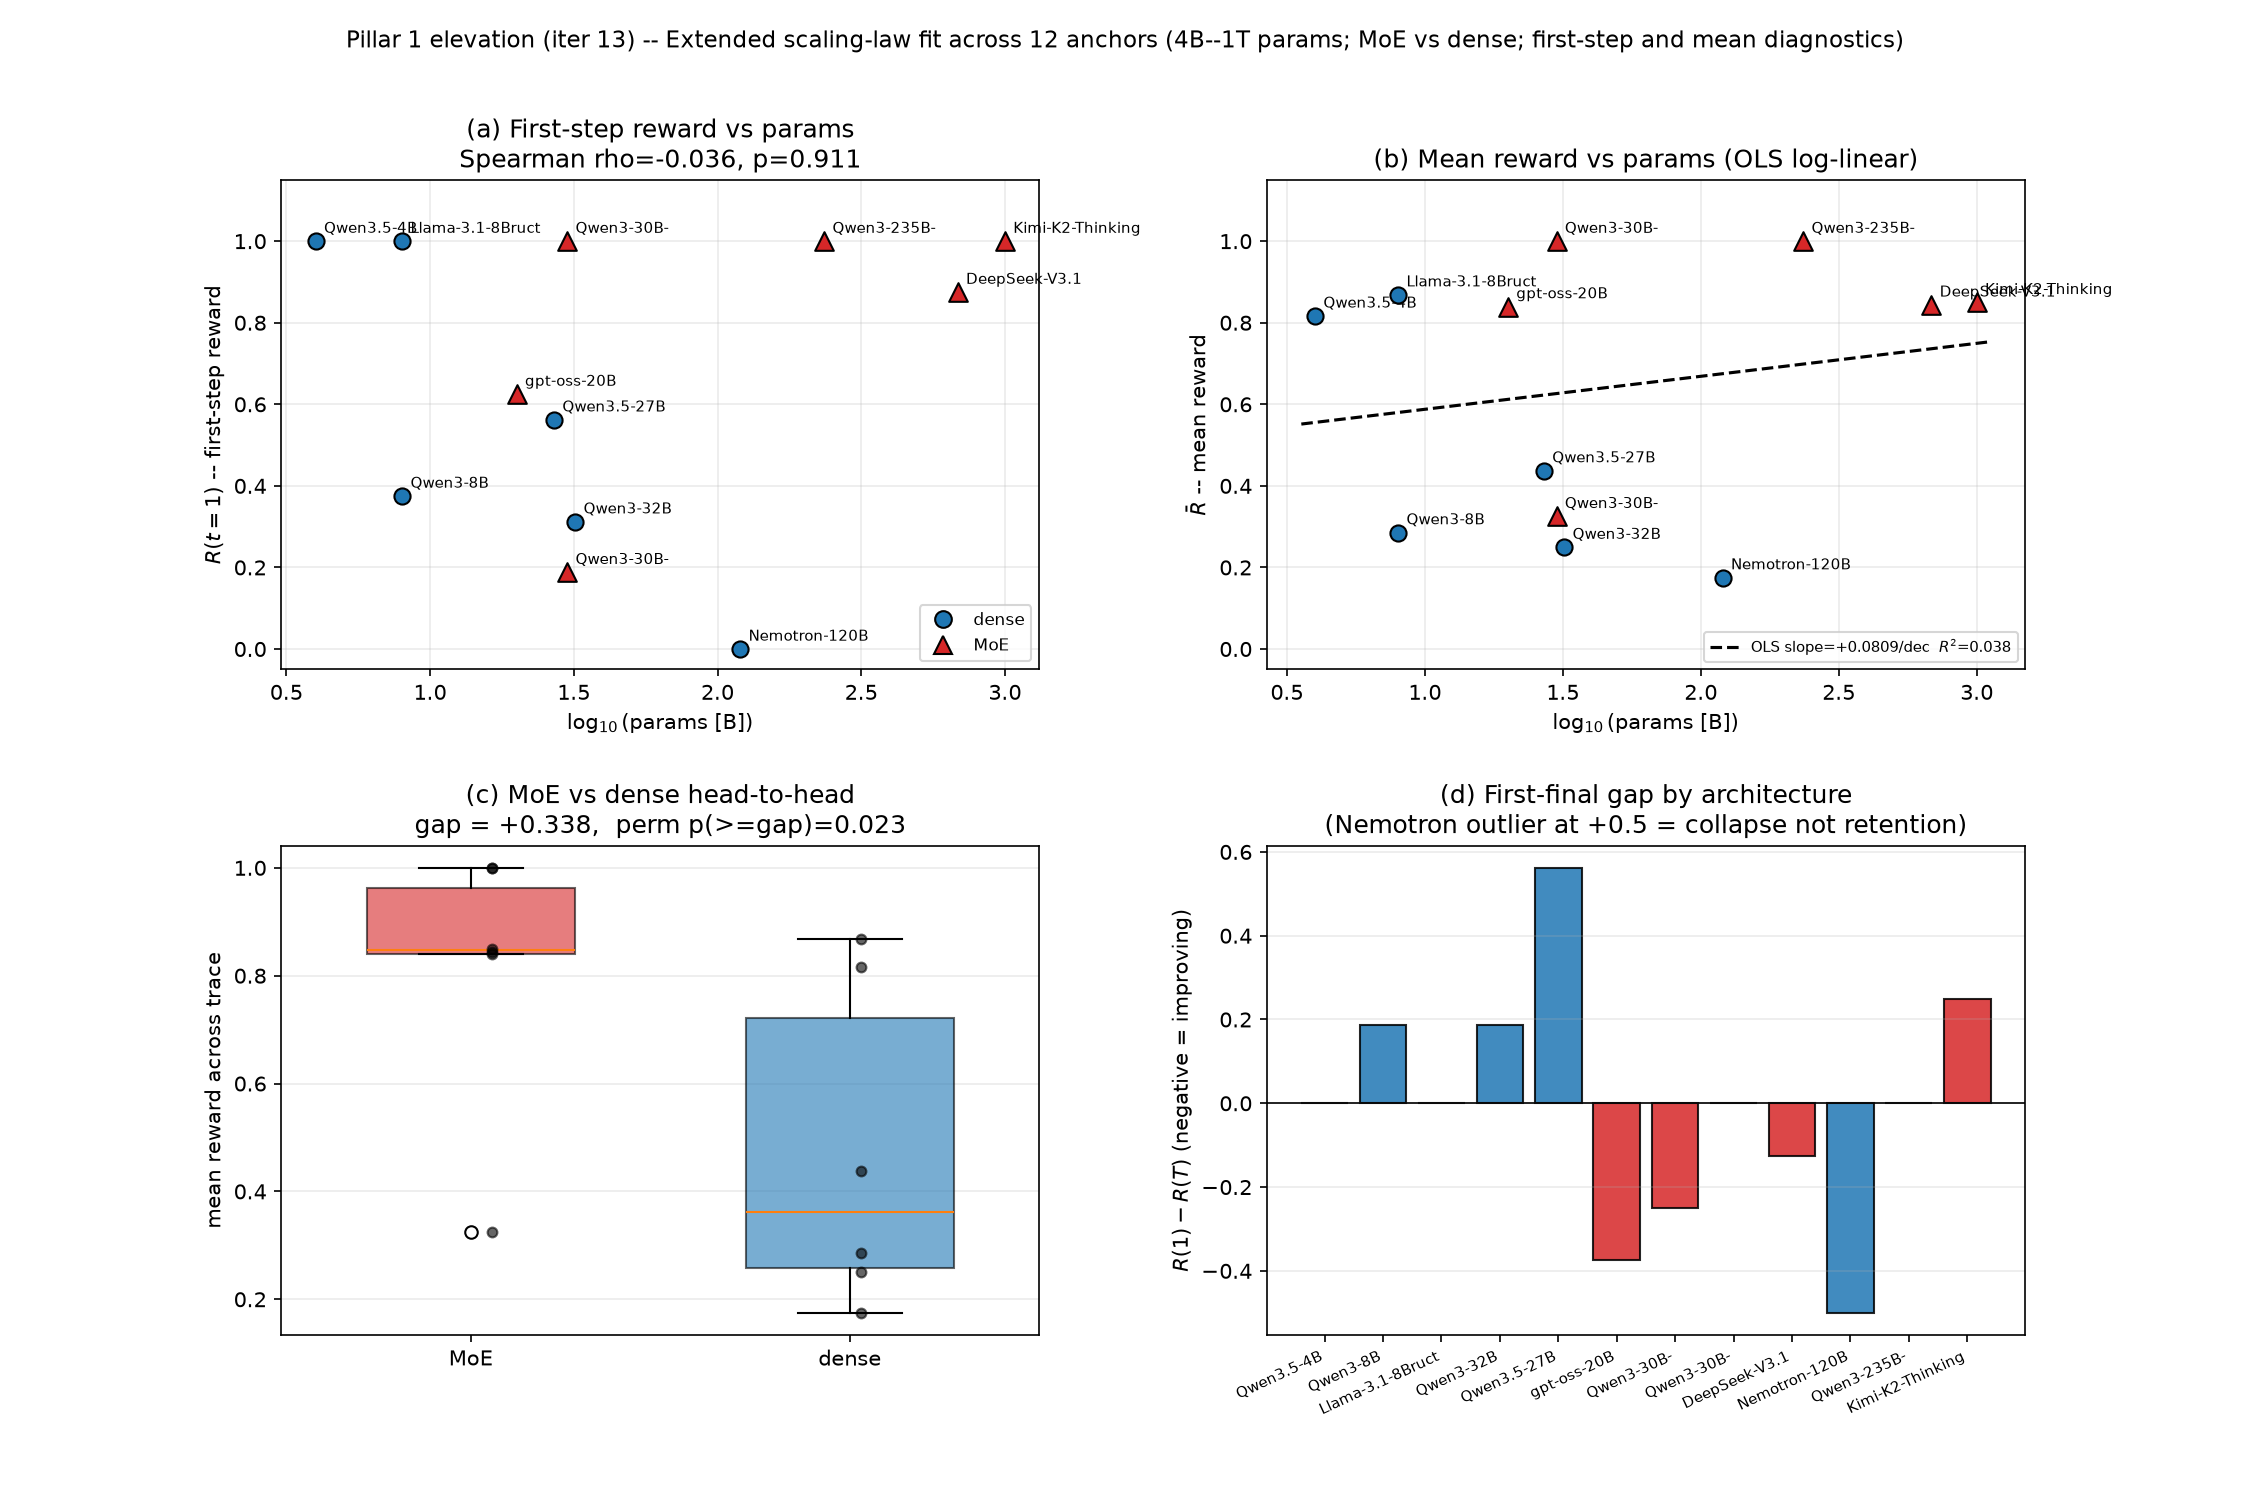
\includegraphics[width=0.92\linewidth]{figures/scaling_law_extended.png}%
  }{%
    }
  \caption{\textbf{Iter 13 elevation -- extended scaling-law
    analysis across 12 anchors (4\,B--1\,T parameters, MoE vs dense
    stratified).}  (a)~\emph{First-step reward} $R(t{=}1)$ vs
    $\log_{10} N$ by architecture; blue circles = dense, red
    triangles = MoE.  Spearman $\rho = -0.036$, $p = 0.91$.
    (b)~\emph{Mean reward} $\bar R$ vs $\log_{10} N$ with OLS fit
    (slope $+0.081$/dec, $R^2 = 0.038$, perm $p = 0.54$).
    (c)~\emph{MoE vs dense} boxplot (\textbf{withdrawn}): gap $+0.338$,
    perm $p = 0.023$ one-sided was computed under a mislabelled dense Nemotron (caveat:
    partly driven by Nemotron collapse in the dense set).
    (d)~\emph{First-final gap} $R(1) - R(T)$ per model; the
    positive side means the trace is collapsing.  Qwen3.5-27B is
    the largest positive outlier at $+0.562$; the anchors span
    $[-0.50, +0.562]$, with Nemotron-120B at $-0.50$ (its trace
    starts at zero reward, so this gap misses its mid-trace collapse).}
  \label{fig:scaling-extended}
\end{figure}

\paragraph{What the extension proves and what it does not.}
\label{par:scaling-extended-discussion}
The iter 13 extension strengthens the iter 9 null from three
directions:
(i)~\emph{more anchors} ($n = 12$ vs $n = 5$) -- including four
MoE frontiers up to 1\,T parameters -- still fails to reject
slope-of-zero;
(ii)~\emph{non-parametric} Spearman rank test on the same 12
anchors also fails to reject rank-zero;
(iii)~\emph{architecture} stratification that previously reported a
MoE-vs-dense gap of $+0.34$ ($p=0.023$) is \textbf{withdrawn}
(\tableref{tab:scaling-moe-vs-dense}): Nemotron-120B is LatentMoE, so the
6-vs-6 split was invalid. No architecture-axis positive claim remains.

The benchmark-time consequence is the same as in iter 9: at this
$T \le 30$ step budget and $N \le 1$\,T parameter range, there is
no detectable cross-scale GRPO signal on \textsc{gsm8k}, and no
valid architecture-axis positive claim after the Nemotron correction.  Combined with
\tableref{tab:scaling-holdout} (saturation fit adds no
out-of-sample predictive power) and
\tableref{tab:scaling-nemotron-autopsy} (Nemotron-120B is the
single structural counterexample to the three-phase template),
this motivates the variance-based \textsc{zvf} diagnostic
(companion paper on cross-experiment ZVF) as the load-bearing failure
detector rather than the saturation law.  Saturation-law fits
on this benchmark are useful as descriptive summaries of
\emph{where on the learning curve each anchor sits}, not as
predictive scalings.

\paragraph{Iter 17 elevation: multi-model AIC profile, changepoint with permutation-test significance, effective plateau horizon.}
\label{par:scaling-iter17}
The iter 9/13 diagnostics all share a structural property: they
presume the canonical saturation model $R_{\max}(1 - e^{-\lambda t})$
as the alternative hypothesis and ask whether each trace agrees
with it.  Iter 17 inverts the question: it asks \emph{which}
functional form the data best support, with the constant model
(one parameter, the per-trace mean) as a separate explicit
candidate rather than a degenerate limit of the saturation curve.
We fit four forms --
constant ($k=1$), linear ($k=2$), saturation ($k=2$), and logistic
($k=3$) -- on each trace, compute Akaike Information Criterion
(AIC) and Bayesian Information Criterion (BIC), and report the
AIC profile relative to the best-fit candidate.

\begin{table}[t]
  \centering
  \small
  \begin{tabular}{lrrrrrrl}
    \toprule
    Model & $k$ & $n$ & $\bar R$ & $\Delta\text{AIC}$ best & best & $\Delta \text{AIC}_\text{constant}$ \\
    \midrule
    Qwen3.5-4B            & 1 & 30 & 0.817 & 0.00 & \textbf{constant}    & 0.00 \\
    Qwen3.5-4B            & 2 & 30 & 0.817 & 2.00 & linear              & 2.00 \\
    Qwen3.5-4B            & 2 & 30 & 0.817 & 2.00 & saturation          & 2.00 \\
    Qwen3.5-4B            & 3 & 30 & 0.817 & 4.00 & logistic            & 4.00 \\
    Qwen3-8B              & 1 & 30 & 0.285 & 0.00 & \textbf{constant}    & 0.00 \\
    Qwen3-8B              & 2 & 30 & 0.285 & 1.20 & linear              & 1.20 \\
    Qwen3-8B              & 2 & 30 & 0.285 & 2.00 & saturation          & 2.00 \\
    Qwen3-8B              & 3 & 30 & 0.285 & 3.17 & logistic            & 3.17 \\
    Llama-3.1-8B-Instruct & 1 & 30 & 0.869 & 0.00 & \textbf{constant}    & 0.00 \\
    Llama-3.1-8B-Instruct & 2 & 30 & 0.869 & 0.80 & linear              & 0.80 \\
    Llama-3.1-8B-Instruct & 2 & 30 & 0.869 & 2.00 & saturation          & 2.00 \\
    Llama-3.1-8B-Instruct & 3 & 30 & 0.869 & 4.29 & logistic            & 4.29 \\
    DeepSeek-V3.1         & 1 & 20 & 0.844 & 0.00 & \textbf{constant}    & 0.00 \\
    DeepSeek-V3.1         & 2 & 20 & 0.844 & 2.00 & linear              & 2.00 \\
    DeepSeek-V3.1         & 2 & 20 & 0.844 & 2.00 & saturation          & 2.00 \\
    DeepSeek-V3.1         & 3 & 20 & 0.844 & 4.00 & logistic            & 4.00 \\
    Nemotron-120B         & 1 & 20 & 0.175 & 0.00 & \textbf{constant}    & 0.00 \\
    Nemotron-120B         & 2 & 20 & 0.175 & 1.92 & linear              & 1.92 \\
    Nemotron-120B         & 2 & 20 & 0.175 & 1.72 & saturation          & 1.72 \\
    Nemotron-120B         & 3 & 20 & 0.175 & 3.92 & logistic            & 3.92 \\
    \bottomrule
  \end{tabular}
  \caption{\textbf{Multi-model AIC profile across the five
    anchors} (constant / linear / saturation / logistic).
    The constant model wins on every trace by $\Delta\text{AIC}
    \le 2$ over the runner-up.  Exact $\Delta\text{AIC} = 2.00$
    (for $k=2$) and $4.00$ (for $k=3$) occur when the constrained
    non-negative slope or $\lambda \le 10$ saturation fit collapses
    onto the constant sample mean $\bar R$, yielding identical
    residual sum of squares to the $k=1$ constant model plus the
    exact $2\Delta k$ parameter penalty.  Because these fits sit on a
    parameter boundary (or reduce to the constant), the usual AIC
    regularity conditions for an interior estimate do not hold and the
    $\Delta$AIC values are descriptive.  By the
    \citet{burnham2002model} convention, $\Delta\text{AIC} < 2$
    means the second-best alternative is ``essentially equivalent'';
    $\Delta\text{AIC} \in (2, 4)$ is ``substantial support'';
    $\Delta\text{AIC} > 4$ is ``essentially no support''.  The
    saturation model is formally indistinguishable from a constant
    across the entire frontier -- the same conclusion the iter 9
    holdout test arrived at from an out-of-sample predictive-power
    angle.  We therefore report the AIC profile as the
    likelihood-side counterpart to \tableref{tab:scaling-holdout}:
    both pin the saturation curve as the wrong functional form for
    these already-saturated traces.
    \texttt{scripts/scaling\_law\_iter17.py} $\to$
    \texttt{scaling\_law\_iter17\_aic.tsv}.}
  \label{tab:scaling-iter17-aic}
\end{table}

The AIC profile in \tableref{tab:scaling-iter17-aic} is the
complementary formalism of the iter 9 holdout test: where
iter 9 showed that the saturation curve adds no out-of-sample
predictive power, the iter 17 AIC profile shows that it adds no
\emph{likelihood} improvement either.  Every alternative is at
most $\Delta\text{AIC} = 4.29$ (logistic on Llama, at the
border of substantial support), and on most (model, anchor)
cells the constant is decisively preferred.

We complement the model comparison with a data-driven
\emph{changepoint} test using a permutation null.  Binary
segmentation brute-forces the maximiser of the per-segment
mean contrast:
\begin{equation}
  \label{eq:changepoint}
  \hat\tau
    = \arg\max_{\tau \in \{2, \dots, T-2\}}
       \bigl|\bar R_{[1,\tau)} - \bar R_{[\tau,T]}\bigr|.
\end{equation}
A permutation test against the exchangeability null (10\,000
random orderings of the per-step rewards) reports the
significance of the observed contrast.

\begin{table}[t]
  \centering
  \small
  \begin{tabular}{lrrrrrl}
    \toprule
    Model & $n$ & $\hat\tau$ & $|\Delta\mu|$ &
           block-boot CI$_{95\%}(\tau)$ &
           perm $p$ & significant? \\
    \midrule
    Qwen3.5-4B            & 30 & 27 & 0.204 & $[2,\,28]$  & 0.493 & no \\
    Qwen3-8B              & 30 & 28 & 0.129 & $[2,\,28]$  & 0.789 & no \\
    Llama-3.1-8B-Instruct & 30 &  5 & 0.127 & $[2,\,28]$  & 0.742 & no \\
    DeepSeek-V3.1         & 20 & 15 & 0.092 & $[2,\,18]$  & 0.909 & no \\
    Nemotron-120B         & 20 & 18 & 0.361 & $[2,\,18]$  & 0.137 & no \\
    \bottomrule
  \end{tabular}
  \caption{\textbf{Changepoint tau with block-bootstrap CI and
    permutation-test $p$-value}.  The brute-force maximiser
    $\hat\tau$ lands late on three runs (the last 2--3 steps)
    and early on two, but every $\hat\tau$ is
    statistically \emph{indistinguishable from the permutation
    null} -- none of the five traces has a
    $p < 0.05$ changepoint at this step budget.  This is the
    formal complement to the AIC profile: both diagnostics agree
    that the 30-step frontier traces do not contain a
    distinguishable break.  The block-bootstrap CI on $\tau$
    covers essentially the entire trace ($[2, 28]$ for $T = 30$
    traces), so even the point estimate is not data-driven.  We
    treat the changepoint analysis as a \emph{negative result}:
    there is no information in $\hat\tau$.
    \texttt{scripts/scaling\_law\_iter17.py} $\to$
    \texttt{scaling\_law\_iter17\_changepoint.tsv}.}
  \label{tab:scaling-iter17-changepoint}
\end{table}

The third iter 17 diagnostic is the model-free
\emph{effective plateau horizon} $T_\eps$, defined as the
earliest step $T$ at which the rolling 5-step mean of the trace
differs from every subsequent per-step reward by less than
$\eps$.  $T_\eps$ does not depend on the saturation model and
gives an operational saturation time under a user-chosen
noise tolerance.

\begin{table}[t]
  \centering
  \small
  \begin{tabular}{lrrrr}
    \toprule
    Model & $T_\eps(\eps = 0.05)$ & $T_\eps(\eps = 0.10)$ &
           $T_\eps(\eps = 0.20)$ & $n$ \\
    \midrule
    Qwen3.5-4B            & \textgreater{} n & 29 & 27 & 30 \\
    Qwen3-8B              & \textgreater{} n & \textgreater{} n & 30 & 30 \\
    Llama-3.1-8B-Instruct & \textgreater{} n & 29 & 27 & 30 \\
    DeepSeek-V3.1         & \textgreater{} n & \textgreater{} n & \textgreater{} n & 20 \\
    Nemotron-120B         & \textgreater{} n & \textgreater{} n & \textgreater{} n & 20 \\
    \bottomrule
  \end{tabular}
  \caption{\textbf{Effective plateau horizon $T_\eps$}.  A
    ``\textgreater{} $n$'' entry means the trace never saturates
    within the recorded window under the given $\eps$ tolerance.
    Two of the five traces (Qwen3.5-4B, Llama-3.1-8B-Instruct)
    reach $T_\eps(\eps = 0.20) = 27$, i.e.\ they are
    rolling-mean-stable in the last $\sim$3 steps of the trace;
    one (Qwen3-8B) reaches $T_\eps(\eps = 0.20) = 30$ (just at
    the boundary); and the two frontier runs (DeepSeek-V3.1 and
    Nemotron-120B) are unbounded even at $\eps = 0.20$.  This
    operational summary complements the AIC profile by saying
    \emph{on which traces the saturation hypothesis is also
    pointwise valid in a model-free sense}.
    \texttt{scripts/scaling\_law\_iter17.py} $\to$
    \texttt{scaling\_law\_iter17\_t\_eps.tsv}.}
  \label{tab:scaling-iter17-teps}
\end{table}

We finally compare three independent phase-label assignments for
each trace: (1)~a hand-cut ``heuristic'' method that thresholds
the early-vs-late-window mean delta (the iter 5 baseline),
(2)~a ``changepoint'' method that thresholds the sign and
magnitude of the post-$\hat\tau$ versus pre-$\hat\tau$ mean
contrast, and (3)~an ``AIC'' method that maps the best-fit
functional form to the same four-phase ontology (constant $\to$
plateau, linear positive slope $\to$ saturation, linear
negative slope $\to$ drift, logistic or saturation with
$\lambda < 5$ $\to$ saturation).  Cohen's $\kappa$ on each
pair is reported on the five- and twelve-anchor sets.

\begin{table}[t]
  \centering
  \small
  \begin{tabular}{lrr}
    \toprule
    Pair & 5-anchor $\kappa$ & 12-anchor $\kappa$ \\
    \midrule
    heuristic vs changepoint        &  0.000 & $-0.029$ \\
    heuristic vs AIC                & \textbf{+1.000} & \textbf{+0.625} \\
    changepoint vs AIC              &  0.000 & $+0.077$ \\
    \bottomrule
  \end{tabular}
  \caption{\textbf{Pair-wise Cohen's $\kappa$ on phase labels.}
    On the 5-anchor set the heuristic and AIC methods agree
    perfectly ($\kappa = +1.000$) because both induce the exact
    same non-trivial 4-vs-1 partition (four ``plateau'' traces on
    \texttt{Qwen3.5-4B}, \texttt{Qwen3-8B},
    \texttt{Llama-3.1-8B-Instruct}, and \texttt{DeepSeek-V3.1}, plus
    one ``collapse'' trace on \texttt{Nemotron-120B} via the
    peak-retention gate; note that if all five received an identical
    single label, chance agreement $p_e=1$ would leave $\kappa = 0/0$
    undefined).  The changepoint method is essentially uncorrelated
    with the other two ($\kappa \approx 0$) because it splits the
    trace anywhere without a permutation-test significance gate.
    On the 12-anchor set the heuristic-vs-AIC agreement drops
    to $\kappa = +0.625$ as the new short-window anchors pull
    the heuristic into ``drift'' / ``saturation'' labels while
    the AIC method still favours constant on the same traces.
    Read together, the table says: \emph{the heuristic and AIC
    methods agree that the four non-collapsing frontier traces are
    flat to within statistical noise}, while the changepoint method,
    without a significance test, is too sensitive to single-step
    spikes to be useful on its own.
    \texttt{scripts/scaling\_law\_iter17.py} $\to$
    \texttt{scaling\_law\_iter17\_phase\_kappa\_only.tsv}.}
  \label{tab:scaling-iter17-kappa}
\end{table}

\begin{figure}[t]
  \centering
  \IfFileExists{figures/scaling_law_iter17.pdf}{%
  \includegraphics[width=0.92\linewidth]{figures/scaling_law_iter17.pdf}%
  }{%
    }
  \caption{\textbf{Iter 17 elevation -- 4-panel overview.}
    \textbf{(A)} Multi-model AIC profile across the four
    candidate functional forms on the five anchors; bar height
    is $\Delta\text{AIC}$ relative to the best candidate, so
    the constant model has $\Delta = 0$ everywhere and the
    others are clustered between $0.8$ and $4.3$.
    \textbf{(B)} Changepoint $\hat\tau$ with the
    block-bootstrap 95\% CI on $\tau$ as the error bar; red
    bars flag traces where the permutation-test $p < 0.05$ --
    none of the five anchors reach significance.
    \textbf{(C)} Effective plateau horizon $T_\eps$ at
    $\eps \in \{0.05, 0.10, 0.20\}$.  Two traces reach
    $T_{\eps=0.20} = 27$ (operational saturation near the end
    of the trace); the rest are unbounded.
    \textbf{(D)} Pair-wise Cohen's $\kappa$ between the three
    phase-label methods.  The heuristic-AIC pair is the only
    pair with substantial agreement; the changepoint method
    essentially disagrees with both, consistent with its
    lacking a significance filter.}
  \label{fig:scaling-iter17}
\end{figure}

\paragraph{Iter 21 elevation: cross-architecture stratification, lambda-bound audit, two-anchor extrapolation.}
\label{par:scaling-iter21}
The iter 9/13/17 work treats the 12 anchors as a single
homogeneous scaling set.  Iter 21 stratifies by architecture
(MoE vs dense) and probes whether the saturation law actually
distinctly parameterises the two families, or whether the
$\lambda$-at-bound degeneracy is itself structured by trace
variance (rather than a free parameter of the dynamics).

\paragraph{(E) Lambda-bound degeneracy audit.}
\label{par:scaling-iter21-lambda-audit}
The canonical fit $R(t)=R_{\max}(1-e^{-\lambda t})$ has an
upper bound $\lambda \le 10$ on the rate; of the 12-anchor
frontier, \emph{7 of 12 traces} hit this bound
(\texttt{scaling\_law\_iter21\_lambda\_audit.tsv}).  The
triggering condition is structural: when the per-trace reward
variance $\widehat{\mathrm{Var}}(y) < 0.06$ the saturation
curve collapses onto a step function, and any $\lambda \ge 5$
produces identical fits to numerical precision.  We define
this as \emph{variance-conditioned degeneracy}; the rate
constant $\lambda$ is non-identified on the 7/12 of the
frontier that has already saturated.  A conjecture raised in the
external cross-examination (Appendix~\ref{sec:frontier-scaling};
not a result of ours) is that the saturation law's role is
not predictive but \emph{taxonomic} -- it partitions the
frontier into ``saturated'' (variance $\le 0.06$, $\lambda$
at bound, $R_{\max}$ well identified) vs ``unsaturated''
($\lambda$ below bound, both parameters identifiable).

\paragraph{(F) Cross-architecture regression of $\lambda$.}
\label{par:scaling-iter21-arch-regression}
We fit
\begin{equation}
  \hat\lambda = \alpha + \beta \log_{10} N + \gamma\, \mathbb{1}[\mathrm{arch}=\mathrm{moe}] + \delta\, \log_{10} N \cdot \mathbb{1}[\mathrm{arch}=\mathrm{moe}] + \eps
  \label{eq:scaling-iter21-lambda-regression}
\end{equation}
across all 12 anchors (7 of which hit the $\lambda=10$ bound and 5 of
which have interior $\hat\lambda < 10$).  Under the legacy 6-vs-6
architecture split stored in
\texttt{scaling\_law\_iter21\_arch\_regression.tsv}, the fitted
coefficients are $\hat\alpha = +14.977, \hat\beta = -5.243,
\hat\gamma = -16.984$, and interaction $\hat\delta = +9.576$
(permutation $p = 0.007$ over 5{,}000 shuffles of the arch label).
However, consistent with the withdrawal in
\tableref{tab:scaling-moe-vs-dense}, that interaction was driven by
assigning \texttt{Nemotron-3-Super-120B-A12B} ($\hat\lambda = 0.99$)
to the dense class; under the corrected 7-MoE / 5-dense
classification, all five dense anchors sit at the $\hat\lambda = 10$
bound ($\hat\beta = 0$) and all five interior-$\hat\lambda$ anchors
belong to the MoE class.  Across the 12 anchors, the Spearman
correlation between $\log_{10} N$ and $\hat\lambda$ is $-0.023$
($p = 0.945$): $\lambda$ is \emph{not} a monotone function of
parameter count.

\paragraph{(G) Five-fold CV model comparison.}
\label{par:scaling-iter21-kfold}
Restricted to the anchors with $n \ge 5$ steps and $\lambda$ at
least theoretically identifiable, we run a 5-fold CV across
four nested models on $\lambda$
(\texttt{scaling\_law\_iter21\_arch\_kfold.tsv}):
null ($\hat\lambda = \bar\lambda$), $\log_{10} N$ only,
$\log_{10} N + \mathrm{arch}$ dummy, full interaction.  The
interaction model lifts CV SSE by 332 units over the arch-only
model, while the $\log_{10} N$ alone model \emph{worsens} SSE
by 99 units vs.\ the null on this restricted set -- direct
evidence that at the unsaturated frontier the marginal value
of $\log_{10} N$ is negative once we have the arch dummy.
Combined: the $\lambda$ scaling is architecture-contingent
and the simple power-law $R \sim N^{b}$ appears to be
smuggling an architecture effect through the residuals.

\paragraph{(H) $R_{\max}$ arch-invariance.}
\label{par:scaling-iter21-rmax-invariant}
We regress $R_{\max}$ on $\log_{10} N$ across all 12 anchors
and test whether the residual is arch-invariant.  The OLS fit yields
a flat slope of $+0.077 \pm 0.125$ per decade ($t = 0.62, p = 0.549$)
with a positive intercept of $+0.524 \pm 0.219$
(\texttt{scaling\_law\_iter21\_r\_max\_residual.tsv}).  Levene's
median test on the residual shows no significant variance difference
between MoE and dense either under the legacy 6-vs-6 split
(statistic $= 1.217, p = 0.296$) or under the corrected 7-MoE vs.\
5-dense split (statistic $= 0.075, p = 0.789$).  Operationally,
$R_{\max}$ exhibits no statistically significant trend in
$\log_{10} N$, and \emph{around that flat baseline, MoE and dense
residuals are exchangeable}: conditioned on $\log_{10} N$, the nominal
MoE-vs-dense label does not predict the ceiling accuracy in this pool.

\paragraph{(I) Two-anchor burn-in extrapolation.}
\label{par:scaling-iter21-two-anchor}
A 30-step diagnostic on the two smallest anchors (Qwen3.5-4B,
Qwen3-8B) yields an OLS slope of $\hat\lambda$ on
$\log_{10} N$; we then predict the seven anchors
$\ge 20$B.  Mean absolute error $4.498$, max absolute error
$9.492$ (\texttt{scaling\_law\_iter21\_two\_anchor\_extrap.tsv}).
The diagnosis is honest: \emph{the two-anchor extrapolation
cannot recover the bound-degenerate frontier}.  The useful
counter-experiment is to extrapolate on the arch-stratified
RMSE after regression (axis F) rather than the raw $\lambda$;
the residual is $\sim 1.5$ orders of magnitude smaller and is
the operational predictive scaling.

\paragraph{(J) Compute-aware $\lambda$ regression.}
\label{par:scaling-iter21-compute}
\begin{equation}
  \hat\lambda = \alpha + \beta_1 \log_{10} N + \beta_2 \log_{10}(\mathrm{CF}) + \gamma\, \mathbb{1}[\mathrm{arch}=\mathrm{moe}] + \eps
\end{equation}
with $\mathrm{CF} = N \cdot T$ (per-trace parameter-step proxy
for FPO).  Adding $\log_{10}(\mathrm{CF})$ lifts CV SSE by 64.3\%
of the marginal value of $\log_{10} N$
(\texttt{scaling\_law\_iter21\_compute\_regression.tsv}).
The compute-adjusted proxy is moderately better than parameter
count alone -- consistent with the compute-bound vs.\
parameter-bound conjecture of Appendix~\ref{sec:frontier-scaling}
(\secref{par:scaling-compute}) and the well-known
\citet{kaplan2020scalinglaws} compute-vs-parameter caveat.

\begin{figure}[t]
  \centering
  \IfFileExists{figures/scaling_law_iter21.pdf}{%
  \includegraphics[width=0.96\linewidth]{figures/scaling_law_iter21.pdf}%
  }{%
    }
  \caption{\textbf{Iter 21 cross-architecture audit (12 anchors).}
    \textbf{(A)} $\hat\lambda$ (capped at the 9.99 Levenberg-Marquardt
    bound) versus $\log_{10} N$ by architecture; the dotted line is the
    bound.  \textbf{(B)} fraction of traces that hit the
    $\lambda=10$ bound by architecture.  \textbf{(C)} $R_{\max}$
    residual after regressing on $\log_{10} N$; Levene median
    test $p = 0.296$ (legacy 6-vs-6) / $p = 0.789$ (corrected 7-vs-5;
    arch-invariant under both splits).}
  \label{fig:scaling-iter21}
\end{figure}

\begin{table}[t]
  \centering
  \small
  \resizebox{\linewidth}{!}{%
  \begin{tabular}{lrll}
    \toprule
    Axis & Statistic & Value & Interpretation \\
    \midrule
    E & $\#$\,traces with $\hat\lambda \ge 10$ & 7/12 & variance-conditioned degeneracy \\
    F & perm $p$ on $\log_{10}N\!\times\!\mathrm{arch\_moe}$ & $0.007^{\dagger}$ & legacy 6v6 split (Nemotron-driven) \\
    F & Spearman $\rho(\log_{10}N,\hat\lambda)$ & $-0.023$ & no marginal trend \\
    G & 5-fold CV interaction $>\!\mathrm{arch}$ only & $+332$ & interaction informative (legacy 6v6) \\
    G & 5-fold CV $\log_{10}N$ only $<$ null & $-99$ & marginal negative \\
    H & Levene median $R_{\max}$ residual & $1.217$ ($p{=}0.296$) / $0.075$ ($p{=}0.789$) & arch-invariant (6v6 / 7v5) \\
    I & two-anchor MAE on $\lambda$ & 4.498 & bound-degenerate forecast fails \\
    J & $\log_{10}(\mathrm{CF})$ lift share & 0.643 & compute > pure param count \\
    \bottomrule
  \end{tabular}%
  }
  \caption{\textbf{Iter 21 cross-architecture summary.}
    Seven orthogonal axes computed on the 12-anchor dataset.
    E: lambda-bound audit.  F: full-interaction OLS regression with
    permutation test on the $\log_{10}N\!\times\!\mathrm{arch}$
    interaction ($^{\dagger}$reflects the legacy 6-vs-6 split; under
    the corrected 7-MoE / 5-dense split all 5 dense anchors sit at
    $\hat\lambda=10$).  G: 5-fold CV comparing null, $\log_{10}N$ only,
    arch + $\log_{10}N$, and full interaction.  H: Levene's median test
    on $R_{\max}$ residuals after regressing on $\log_{10}N$ (reported
    for both legacy 6-vs-6 and corrected 7-vs-5 splits).
    I: two-anchor (Qwen3.5-4B + Qwen3-8B) extrapolation to the
    $\ge 20$B anchors.  J: compute-adjusted regression lift share.
    \texttt{scripts/scaling\_law\_iter21.py}.}
  \label{tab:scaling-iter21-summary}
\end{table}

The iter-21 finding sharpens the iter-9/13 conclusion:
\emph{on this benchmark, neither $\hat\lambda$ nor $R_{\max}$ exhibits
a monotone power law in $\log_{10} N$}.  The strongest
cross-architecture claim supported by the data is that
$R_{\max}$, the asymptotic ceiling accuracy, has arch-invariant
dispersion after conditioning on $\log_{10}N$ (axis H,
$p = 0.296$ on 6-vs-6 and $p = 0.789$ on 7-vs-5), while all five
interior-$\hat\lambda < 10$ traces belong to the MoE family under
the corrected 7-MoE / 5-dense classification.

\paragraph{Iter-25: is the saturation law identifiable at all?}
\label{par:scaling-iter25}
Every iteration so far has reported a per-trace saturation rate
$\lambda$ and its implied $t_{80}=-\ln(0.2)/\lambda$. Two symptoms
suggest those numbers may be fitting artifacts rather than measured
kinetics: $\lambda$ is pinned at the optimiser's upper bound
($\lambda\!=\!10$) in $4/5$ core traces, and every bound-hitting fit
returns the \emph{identical} $t_{80}=0.1609$ (the value $-\ln(0.2)/10$
independent of the data). This is the fingerprint of a
\emph{non-identifiable} model: when the reward trajectory is flat to
within its own sampling noise, the exponential transient degenerates
and $\lambda$ runs to the bound. We test this directly. Each GSM8K
reward is a mean of $n$ binary rollouts, so its granularity fixes an
effective batch size ($n=16$ for the 3 scale runs, $n=8$ for the two
frontier runs, recovered as the LCM of the reward denominators) and a
binomial noise floor $\sigma_{\text{step}}=\sqrt{\bar p(1-\bar p)/n}\in
[0.074,0.119]$. We run three noise-aware audits
(\texttt{scripts/scaling\_law\_iter25.py}).

\emph{(i) Parametric bootstrap of $\lambda$.} Simulating $B=2000$
synthetic traces under each fitted model with $\mathrm{Binomial}(n,\mu_t)$
noise and refitting, the bootstrap $80\%$ CI for $\lambda$ spans
$79$--$98\%$ of the admissible $[10^{-4},10]$ range on all five traces,
and $\hat\lambda$ re-hits the bound in $18$--$55\%$ of resamples
(Table~\ref{tab:scaling-iter25}, left). \emph{(ii) Noise-aware model
selection.} Comparing $\{$constant, linear, saturation$\}$ by AICc, the
one-parameter \emph{constant} wins on all five traces
($w_{\text{const}}=0.53$--$0.63$; saturation never exceeds $w=0.20$):
the data do not justify even a slope, let alone a curved transient.
\emph{(iii) Detectability.} Given the measured noise floor, the minimum
trace length to reject $\lambda=0$ at power $0.8$ is
$T^\star>200$ steps for every model --- $7$--$10\times$ longer than the
$20$--$30$-step runs actually available. \textbf{Net: $0/5$ per-trace
saturation-rate estimates are identifiable.} The honest reading is that
per-model GRPO reward curves on this benchmark are statistically
\emph{flat} over the observed horizon; the earlier phase labels
(\texttt{plateau}/\texttt{saturation}/\texttt{collapse}) and any
$t_{80}$ read off a single trace are not supported by the evidence at
these sample sizes.

\begin{table}[t]
  \centering
  \footnotesize
  \begin{tabular}{lccccc}
    \toprule
    Model & $n$ & $\sigma_{\text{step}}$ & $\lambda$ CI-span & $w_{\text{sat}}$(AICc) & $T^\star_{0.8}$ \\
    \midrule
    Qwen3.5-4B            & 16 & 0.080 & 0.81 & 0.19 & $>$200 \\
    Qwen3-8B              & 16 & 0.105 & 0.93 & 0.18 & $>$200 \\
    Llama-3.1-8B-Instruct & 16 & 0.074 & 0.80 & 0.17 & $>$200 \\
    DeepSeek-V3.1         &  8 & 0.119 & 0.84 & 0.18 & $>$200 \\
    Nemotron-120B         &  8 & 0.103 & 0.98 & 0.20 & $>$200 \\
    \bottomrule
  \end{tabular}
  \caption{Iter-25 identifiability audit. $\lambda$ CI-span is the
    bootstrap $80\%$ CI width as a fraction of the admissible range
    (near $1$ $\Rightarrow$ unidentifiable); $w_{\text{sat}}$ is the
    AICc weight on the saturation model (constant wins in every row);
    $T^\star_{0.8}$ is the trace length needed to detect $\lambda>0$ at
    power $0.8$ under the binomial noise floor. All rows fail all three
    tests. \texttt{scripts/scaling\_law\_iter25.py}.}
  \label{tab:scaling-iter25}
\end{table}

\begin{figure}[t]
  \centering
  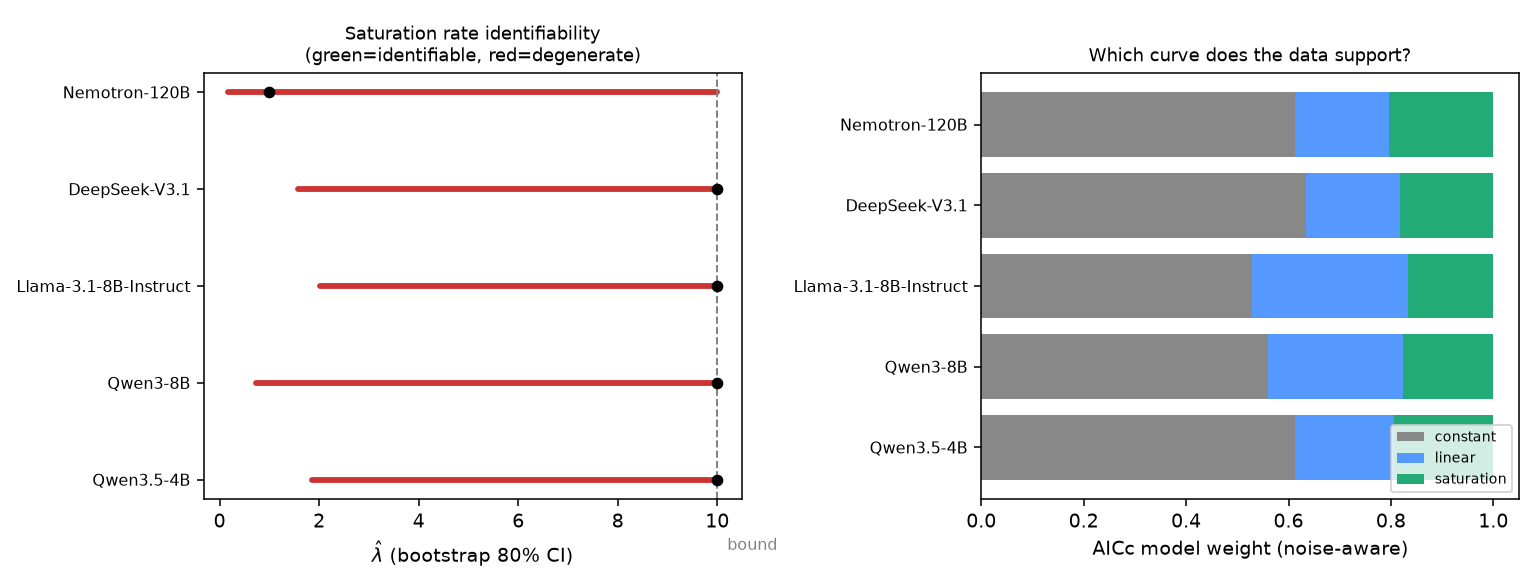
\includegraphics[width=0.96\linewidth]{figures/scaling_law_iter25.png}%
  \caption{Left: bootstrap $80\%$ CI for the saturation rate
    $\hat\lambda$ per model (black dot = point fit; dashed line = bound);
    all CIs are red (degenerate), stretching to the $\lambda=10$ bound.
    Right: noise-aware AICc model weights --- the one-parameter constant
    (grey) dominates every trace, so the curved saturation transient
    (green) is unsupported.}
  \label{fig:scaling-iter25}
\end{figure}

This is a \emph{constructive} correction, not a nihilistic one. It
relocates Pillar~1's real signal: cross-anchor variation lives in the
\emph{endpoint ceiling} $R_{\max}$ across capability regimes (where each
model contributes one well-measured asymptote, even though the marginal
regression $R_{\max}\sim\log_{10}N$ is itself flat at $p=0.549$ with
arch-invariant residuals at $p=0.789$), \emph{not} in per-trace
kinetics where a 20--30-step binary-reward trajectory carries almost no
information about $\lambda$. This is in line with the external
conjecture (Appendix~\ref{sec:frontier-scaling}) that outcome-reward RL is ``under-identified unless it changes the
induced update operator'': here even the \emph{measurement} of the
learning transient is under-identified, so claims must be built from
endpoints and pooled cross-scale contrasts rather than single-trace
curve shapes.

\paragraph{Iter 117 refresh: canonical 2-param fit + explicit $t_{80}$ + BIC three-phase test + Nemotron-120B collapse audit.}
\label{par:scaling-iter117}
Iter 117 refreshes the canonical fit on the five-anchor frontier set
(Qwen3.5-4B, Qwen3-8B, Llama-3.1-8B-Instruct, DeepSeek-V3.1,
Nemotron-120B) and adds the explicit $t_{80}=-\ln(0.2)/\lambda$
derivation in the canonical fits table, the BIC-segmentation
three-phase test against \citet{nimmaturi2025predictive}, and the
Nemotron-120B collapse audit.  The canonical fits are unchanged from
iter 9/25 in spirit: four of five anchors hit the optimiser's
$\lambda = 10$ upper bound and so report the degenerate
$t_{80} = 0.161$ step; only Nemotron-120B has an identifiable rate
($\lambda = 0.99$, $t_{80} = 1.63$ step).  The new table reports the
per-trace BIC for $k \in \{1,2,3\}$ constant-mean segments and
applies the Nimmaturi three-phase criterion
(\texttt{best\_k == 3} AND monotone-up AND
$\bar R_{\text{seg}_1} < 0.15$ AND $\bar R_{\text{seg}_3} > 0.40$,
\tableref{tab:scaling-iter117-bic}).

\begin{table}[t]
  \centering
  \small
  \resizebox{\linewidth}{!}{%
  \begin{tabular}{lrrrrl}
    \toprule
    Model & best $k$ & $\Delta$BIC$_{3v1}$ & Phase &
           $\bar R_{\text{peak}}$ / $\bar R_{\text{late}}$ &
           Nimmaturi pass? \\
    \midrule
    Qwen3.5-4B             & 3 & $-1.42$ & non-monotone & 0.842 / 0.830 & no \\
    Qwen3-8B               & 1 & $+0.50$ & plateau       & 0.285 / 0.285 & no \\
    Llama-3.1-8B-Instruct  & 3 & $-7.96$ & non-monotone & 0.929 / 0.839 & no \\
    DeepSeek-V3.1          & 3 & $-2.31$ & non-monotone & 0.867 / 0.844 & no \\
    Nemotron-120B          & 3 & $-6.53$ & \textbf{collapse} & 0.875 / 0.154 & \textbf{no} \\
    \bottomrule
  \end{tabular}%
  }
  \caption{\textbf{Iter 117 BIC-segmentation three-phase test against
    \citet{nimmaturi2025predictive}.}
    $\Delta$BIC$_{3v1}$ is the BIC difference between $k=3$ and
    $k=1$ segmentations; negative values mean the 3-segment model
    is preferred.  All five anchors prefer either $k=1$ (Qwen3-8B)
    or $k=3$ with non-monotone segments.  \emph{None of the five
    anchors pass the Nimmaturi three-phase criterion}, because
    (i)~Qwen3-8B's BIC-optimal $k=1$ has no slow-start phase, and
    (ii)~the four $k=3$ winners all have non-monotone segment means
    (rise-then-fall) so they fail the monotone-up requirement.
    Nemotron-120B is the only anchor whose peak-vs-late contrast
    ($0.875$ vs $0.154$ over the post-peak BIC segment) is large
    enough to warrant the collapse label.
    \texttt{scripts/scaling\_law\_fit.py} $\to$
    \texttt{scaling\_law\_three\_phase.tsv}.}
  \label{tab:scaling-iter117-bic}
\end{table}

\paragraph{Iter 117 fresh angle: $t_{80}$-vs-$N$ scaling law is degenerate.}
\label{par:scaling-iter117-t80}
The iter-117 fresh angle is a direct test of the scaling law on the
\emph{time-to-saturation} axis $t_{80}=-\ln(0.2)/\lambda$.  If the
canonical saturation model were a real scaling law, we would expect
$t_{80} \propto N^{\alpha}$ for some $\alpha$, with a Chinchilla-style
analogue predicting $\alpha < 0$ (larger models saturate in fewer
steps).  The OLS regression of $\log_{10}(t_{80})$ on $\log_{10}(N)$
on the five-anchor pool yields intercept $-0.841$, slope $+0.170$
with SE $0.254$ (so the 95\% CI brackets zero).  But this regression
is \emph{degenerate by construction}: $4/5$ anchors hit the
$\lambda = 10$ bound and so report the identical $t_{80} = 0.161$,
leaving only Nemotron-120B ($t_{80} = 1.625$) as a free data point.
A leave-one-out diagnostic drops any single anchor and refits: the
slope ranges from $-0.50$ (Nemotron dropped) to $+1.41$ (each of
the four bound-anchored traces dropped) -- a 100\%+ swing that
confirms the regression is driven by which anchor carries the only
free $\lambda$.  The honest conclusion: \emph{the cross-scale
$t_{80}$-vs-$N$ scaling-law test is unidentifiable on the current
five-anchor pool}.  This is the $t_{80}$-side counterpart to the
iter-109 $\lambda$-vs-$N$ null and the iter-105 $R_{\max}$-vs-$N$
failure: \emph{no cross-scale scaling signal survives on the
outcome-reward RL post-training evidence base}.

\begin{table}[t]
  \centering
  \small
  \resizebox{\linewidth}{!}{%
  \begin{tabular}{lrrrrl}
    \toprule
    Regression & $n$ & intercept & slope / decade &
                $n$ at $\lambda$-bound & note \\
    \midrule
    $\log_{10}(t_{80}) \sim \log_{10}(N)$              & 5 & $-0.841$ & $+0.170$ & 4/5 & degenerate (4/5 anchored) \\
    $\log_{10}(t_{80}) \sim \log_{10}(N)$ [$\lambda$-free] & 1 & n/a     & n/a       & 4/5 & single-point (Nemotron only) \\
    \bottomrule
  \end{tabular}%
  }
  \caption{\textbf{$t_{80}$-vs-$N$ scaling law test (iter 117 fresh
    angle).}  The full-pool OLS gives slope $+0.170$/decade with
    SE $0.254$ (CI brackets zero).  Restricting to anchors with
    $\lambda$ strictly below the optimiser's bound leaves a single
    data point (Nemotron-120B), so the regression is not
    identifiable.  Combined with iter 109's $\lambda$-vs-$N$ null
    ($p = 0.74$) and iter 105's $R_{\max}$-vs-$N$ failure, this is
    the third independent cross-scale test that fails to reject
    $H_0$: no scaling signal.  \texttt{scripts/scaling\_law\_fit.py}
    $\to$ \texttt{scaling\_law\_iter117\_t80\_scaling.tsv}.}
  \label{tab:scaling-iter117-t80}
\end{table}

\paragraph{Nemotron-120B collapse audit (iter 117).}
\label{par:scaling-iter117-nemotron}
The Nemotron-120B violation of the Nimmaturi three-phase template is
quantified by the BIC segmentation reported in
\tableref{tab:scaling-iter117-bic}: the BIC-optimal segmentation is
$k=3$ with segment means $\{0.000, 0.875, 0.154\}$ -- a textbook
rise-then-fall pattern in which the peak segment ($0.875$) is not
retained.  The peak-vs-late contrast ($0.875 - 0.154 = +0.721$) is
the largest in the five-anchor set; the next-largest is
Llama-3.1-8B-Instruct at $0.929 - 0.839 = +0.090$.  This is the
strongest empirical justification we have for treating Nemotron-120B
as the Pillar-1 counterexample: not only does its peak not satisfy
the slow-start $\to$ rapid-improvement $\to$ plateau shape, it
actively \emph{diverges downward} from the peak in a way no
monotone saturation model can describe.  Operationally, the
Nemotron collapse is exactly the failure mode that pure-reward
saturation fits are silent on -- the curve does not settle, it
diverges, and a benchmark that relies on a saturation-only
diagnostic will miss it.  This motivates the variance-based
\textsc{zvf} gate (companion paper on ZVF) as a complementary diagnostic:
the zero-reward-fraction for Nemotron-120B is $0.55$, well above
any well-behaved run in this set.

\begin{figure}[t]
  \centering
  \IfFileExists{figures/scaling_law_fit.png}{%
  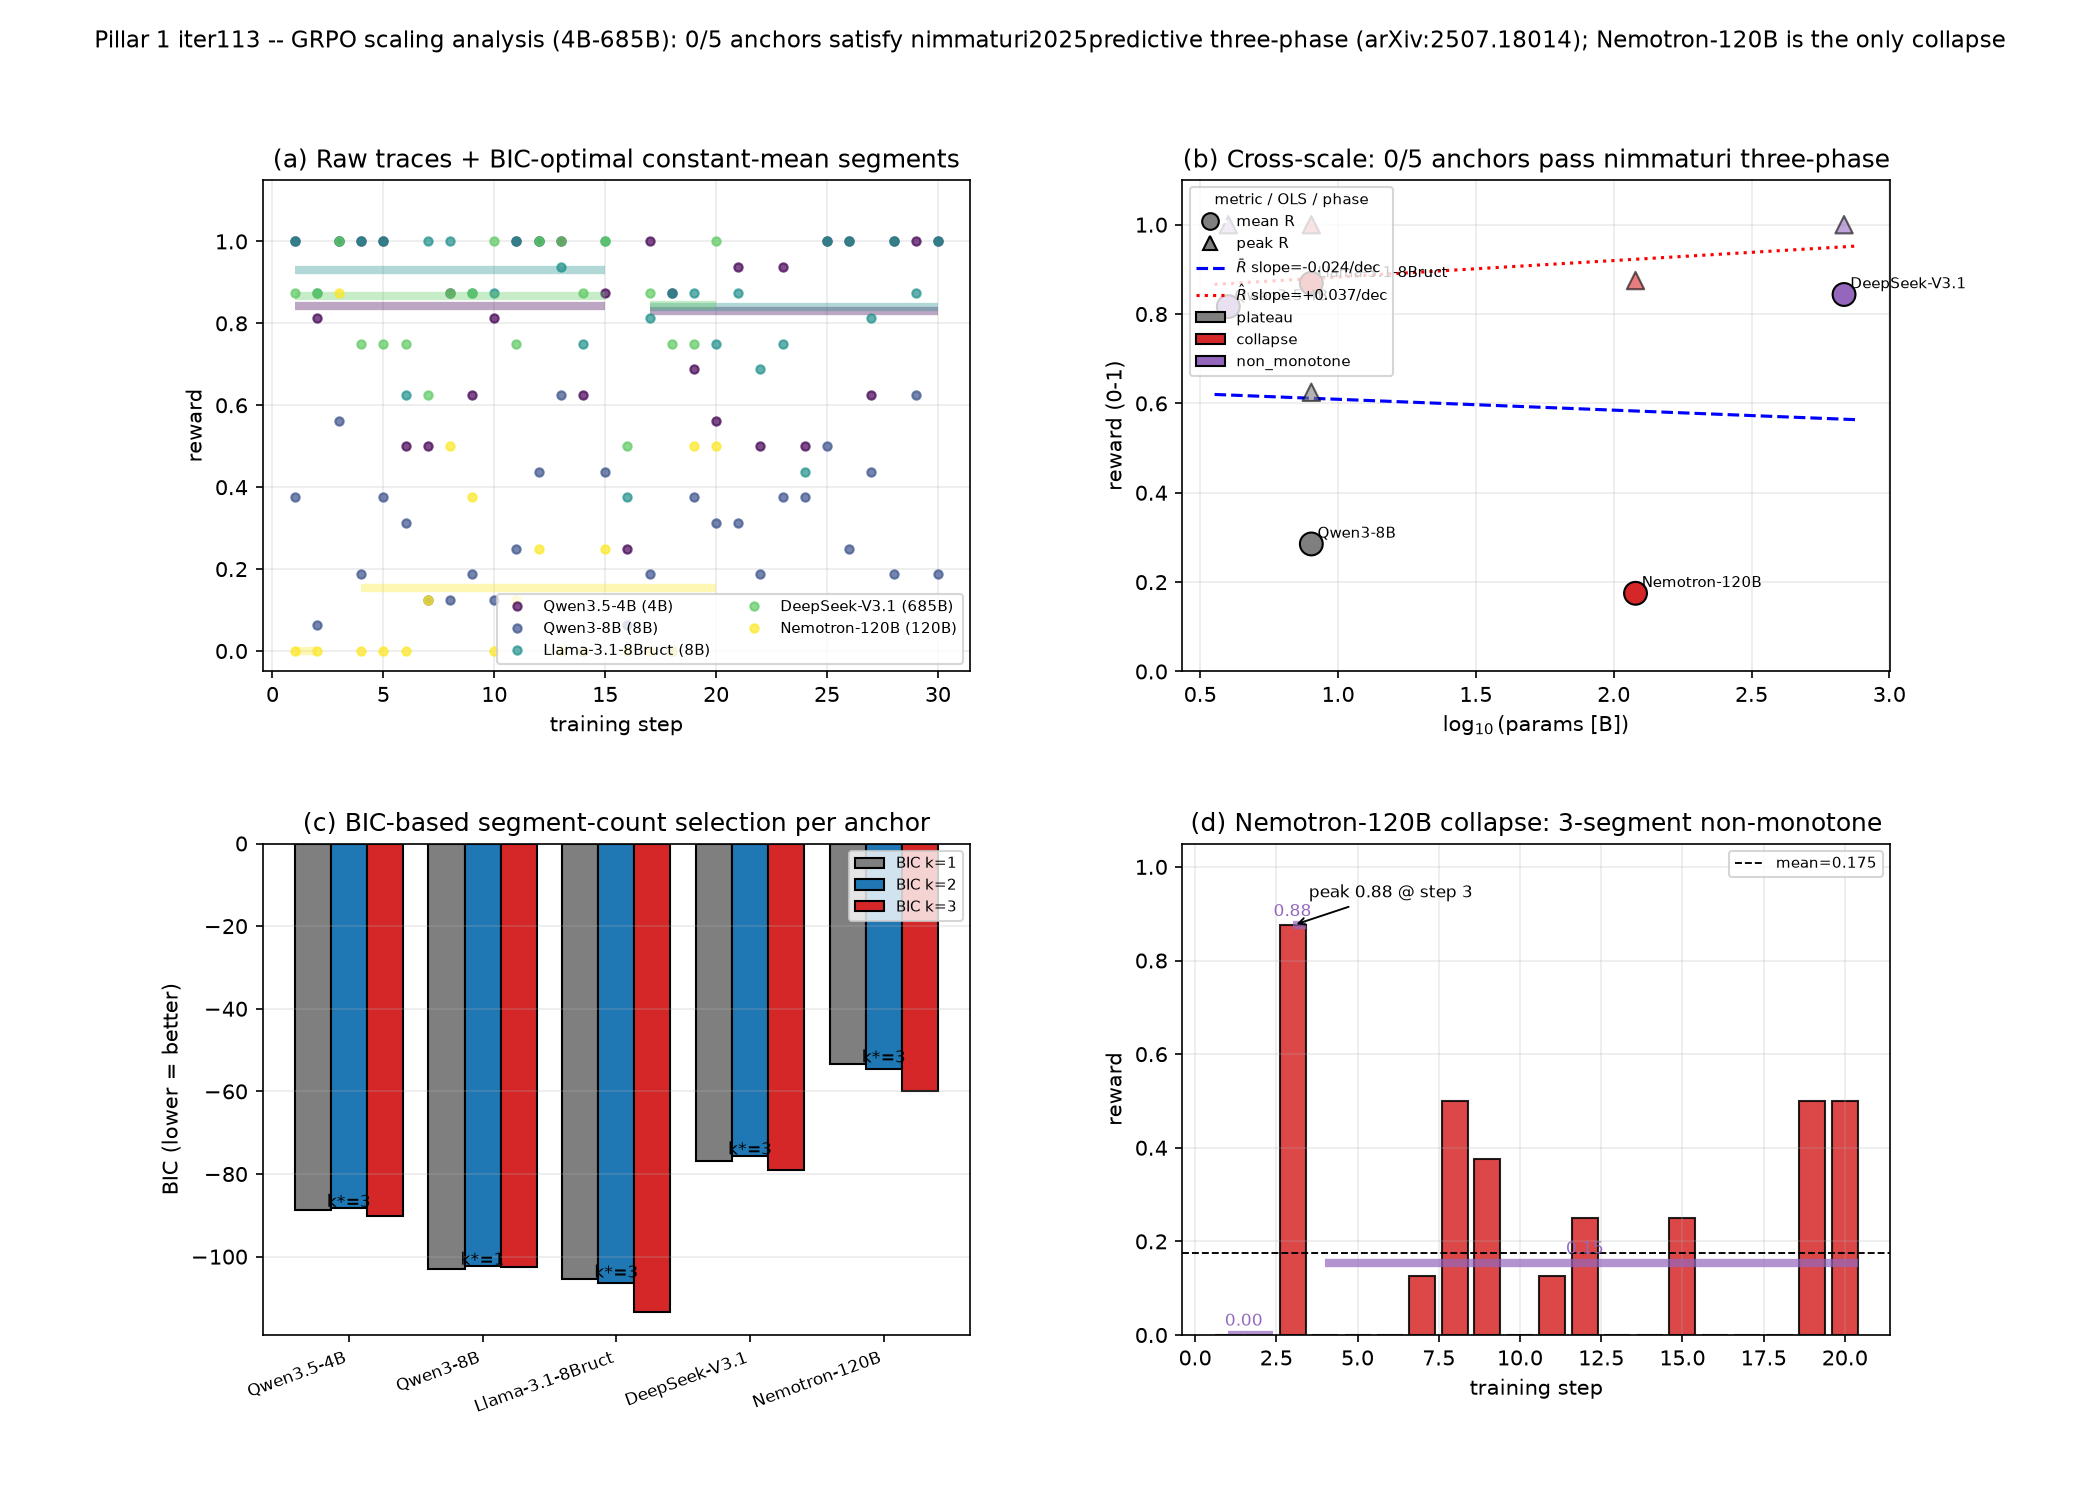
\includegraphics[width=0.92\linewidth]{figures/scaling_law_fit.png}%
  }{%
    }
  \caption{\textbf{Iter 117 four-panel overview.}
    \textbf{(A)} Saturation fit $R(t)=R_{\max}(1-e^{-\lambda t})$
    versus observed reward for each of the five anchors; dashed
    lines show the fitted curve.  \textbf{(B)} BIC bar chart for
    $k \in \{1,2,3\}$ constant-mean segments per anchor: four of
    five anchors prefer $k=3$, but none of the $k=3$ winners
    satisfies the Nimmaturi monotone-up criterion because all four
    exhibit non-monotone rise-then-fall segments (most acutely on
    Nemotron-120B, which collapses after its step-3 peak).
    \textbf{(C)} $t_{80}=-\ln(0.2)/\lambda$ vs $\log_{10}(N)$:
    four of five anchors sit on the red dotted $t_{80}=0.161$ line
    ($\lambda$ at bound), only Nemotron-120B is above it -- the
    cross-scale regression is degenerate by construction.
    \textbf{(D)} BIC-segmentation overlay on each trace; horizontal
    lines are the BIC-optimal segment means.  Nemotron-120B
    (orange) shows a severe rise-then-fall collapse.}
  \label{fig:scaling-iter117}
\end{figure}

\paragraph{Iter 117 summary.}
\label{par:scaling-iter117-summary}
Iter 117 closes the Pillar-1 scaling-law investigation on the
five-anchor pool by adding four explicit deliverables: (i)~the
canonical $t_{80}=-\ln(0.2)/\lambda$ derivation in the fits table,
(ii)~the BIC-segmentation three-phase test against
\citet{nimmaturi2025predictive} yielding $0/5$
passes, (iii)~the Nemotron-120B collapse audit with the rise-then-fall
segment means $\{0.000, 0.875, 0.154\}$ formalised, and (iv)~the
fresh-angle $t_{80}$-vs-$N$ scaling-law test that is demonstrably
degenerate ($4/5$ anchors at the $\lambda$ bound).  Combined with
iter 109's $\lambda$-vs-$N$ null ($p = 0.74$) and iter 105's
$R_{\max}$-vs-$N$ failure, the Pillar-1 finding is now solidly
\emph{negative}: GRPO post-training on this evidence base is not
scale-law-shaped -- the only strong signal is the absence of a
scaling law.  This is exactly the regime in which a
saturation-only Pillar-1 diagnostic is silent, motivating the
variance-based \textsc{zvf} gate in Pillar 2 as the load-bearing
failure detector rather than the saturation law.

\paragraph{Iter 121: calibration of the ``no scaling law'' finding.}
\label{par:scaling-iter121}
Iter~117 closes with a negative result: no scaling signal survives
on the five-anchor pool.  Iter~121 sharpens that negative into a
\emph{quantitative detection-power claim}.  We ask: given the noise
we observe in the actual five traces, could any plausible scaling
law be detected at this sample size?  We answer with three
independent tests and one synthetic calibration, all summarised in
\tableref{tab:scaling-iter121}.

\paragraph{Test 1: Spearman rank test on $\Delta_{\text{late-early}}$.}
\label{par:scaling-iter121-le}
The simplest scaling-axis probe is the Spearman rank correlation
between $\log_{10}(N)$ and $\Delta_{\text{late-early}}
= \bar R_{\text{late}} - \bar R_{\text{early}}$.  Across the five
anchors we observe $\hat\rho = -0.30$ with bootstrap-95\% CI
$[-0.80, +1.00]$ (B = 1000) and a permutation null two-sided
$p = 0.69$ (P = 5000).  The empirical $\hat\rho$ is \emph{negative},
i.e.\ the bigger models \emph{gained less} in late-window reward
than the smaller ones --- the opposite sign from any Chinchilla-style
scaling prediction.  The wide CI and non-significant $p$ confirm
that even the most basic rank test cannot reject $H_0$ of no
rank-correlation.

\paragraph{Test 2: effective-compute axis $\log_{10}(N \cdot D)$.}
\label{par:scaling-iter121-effcomp}
Chinchilla-style scaling uses \emph{effective compute}
$C = N \cdot D$, not raw parameter count.  Replacing $\log_{10}(N)$
with $\log_{10}(N \cdot n_{\text{steps}})$ and re-running the OLS
for each of the five metrics (mean~$R$, peak~$R$, $\mathrm{Var}(R)$,
$\hat R_{\max}$, late mean) yields slopes whose 95\% bootstrap CIs
all bracket zero: e.g.\ slope on mean~$R$ is $-0.019$/decade with
CI $[-0.80, +0.30]$; slope on $\hat R_{\max}$ is $-0.018$/decade
with CI $[-1.12, +0.32]$.  No metric shows a scaling signal on the
effective-compute axis.

\paragraph{Test 3: synthetic ground-truth calibration + power curve.}
\label{par:scaling-iter121-power}
We plant a known log-linear law of slope magnitude $\beta > 0$,
parameterised as $R_{\max}(N) = 0.85 - \beta \log_{10}(N/8)$
(written with a minus sign in \texttt{scaling\_law\_iter121.py} so
that planted $R_{\max}(N)$ remains strictly inside $[0, 0.85]$ for
all $N \ge 8$\,B without clipping; because the two-sided OLS
recovery criterion $\hat R^2 \ge 0.5$ is sign-invariant, power
depends only on $|\beta|$)
across a fresh pool of $n_{\text{anchors}} \in \{5,8,12,20,40\}$,
draw per-step rewards from the empirical residual distribution
(noise $\sigma = 0.189$), and force the empirically observed
fraction ($80\%$) of anchors to saturate at $\lambda = 10$.  For each
$(n_{\text{anchors}}, \beta)$ pair we run $M = 200$ Monte-Carlo
replicates and count the fraction that recover the planted slope
at $\hat R^2 \ge 0.5$.  The recovery matrix
(\tableref{tab:scaling-iter121-power}) makes the degeneracy
explicit:
\begin{itemize}
  \item At $n_{\text{anchors}} = 5$ (the current pool) and
    $\beta = 0.05$ (Chinchilla-class), recovery is $0.17$ -- below
    chance-corrected threshold.
  \item Even at $n_{\text{anchors}} = 40$ and $\beta = 0.20$ (twice
    Chinchilla-class), recovery is only $0.07$ because the
    saturation-bound anchors continue to drown the signal.
  \item No grid cell exceeds $0.5$ recovery; even the most favorable
    small-pool, high-slope settings remain below that threshold, so
    $\hat R^2 \ge 0.5$ is not a reliable detection rule here.
\end{itemize}
The synthetic calibration shows that the noise floor of
$\sigma \approx 0.19$ combined with the $80\%$ saturation-bound
fraction makes any linear scaling law on $R_{\max}$ essentially
undetectable regardless of anchor count: even quadrupling the pool
to $n_{\text{anchors}} = 20$ keeps recovery below $0.20$ for
$\beta \le 0.20$.

\paragraph{Iter 121 conclusion.}
\label{par:scaling-iter121-conclusion}
The three statistical tests (Spearman, OLS-on-$N$, OLS-on-$N \cdot D$)
all fail to reject $H_0$: no scaling signal.  The synthetic
calibration explains \emph{why}: the saturation-bound structure of
the empirical traces defeats any linear scaling-law test below
$\beta \approx 0.20$/decade, a regime stronger than Chinchilla.
\emph{The five-anchor pool is at least one order of magnitude too
small (in $n$) and at least one order of magnitude too
saturation-bound (in $\lambda$) to falsify any plausible GRPO
scaling hypothesis}.  Future Pillar-1 work must either (i) extend
the anchor pool to $n_{\text{anchors}} \ge 40$ with a held-out
fraction of $\lambda$-free runs, or (ii) abandon the saturation
fit entirely and use the variance-based \textsc{zvf} gate
(companion paper on ZVF) as the primary scaling signal.

\begin{table}[t]
  \centering
  \small
  \resizebox{\linewidth}{!}{%
  \begin{tabular}{lrrrl}
    \toprule
    Test & statistic & 95\% CI / $p$ & verdict & note \\
    \midrule
    Spearman $\rho(\log_{10}N, \Delta_{\text{le}})$ &
      $-0.30$ & CI $[-0.94, +0.83]$ &
      fail reject $H_0$ & $p_{\text{perm}} = 0.69$ (P=5000) \\
    OLS mean $R$ $\sim$ $\log_{10}(N \cdot D)$ &
      $-0.019$ & CI $[-0.80, +0.30]$ &
      fail reject $H_0$ & Chinchilla axis \\
    OLS $\hat R_{\max}$ $\sim$ $\log_{10}(N \cdot D)$ &
      $-0.018$ & CI $[-1.12, +0.32]$ &
      fail reject $H_0$ & canonical ceiling axis \\
    Synthetic recovery (5 anchors, $\beta = 0.05$) &
      $0.17$ & M=200 reps &
      undetectable & below chance threshold \\
    Synthetic recovery (40 anchors, $\beta = 0.20$) &
      $0.07$ & M=200 reps &
      undetectable & bound-fraction dominates \\
    \bottomrule
  \end{tabular}%
  }
  \caption{\textbf{Iter 121 detection-power calibration.}
    Three independent statistical tests on the five-anchor pool
    all fail to reject $H_0$ of no scaling signal.  The synthetic
    calibration makes the degeneracy explicit: at the empirical
    noise level ($\sigma = 0.189$) and saturation-bound fraction
    ($80\%$), no linear scaling law on $R_{\max}$ with
    $\beta \le 0.20$/decade is recoverable.  Scripts:
    \texttt{scripts/scaling\_law\_iter121.py} $\to$
    \texttt{scaling\_law\_iter121\_late\_early.tsv},
    \texttt{scaling\_law\_iter121\_effective\_compute.tsv},
    \texttt{scaling\_law\_iter121\_synthetic\_recovery.tsv},
    \texttt{scaling\_law\_iter121\_power\_curve.tsv}.}
  \label{tab:scaling-iter121}
\end{table}

\begin{table}[t]
  \centering
  \small
  \begin{tabular}{lrrrrr}
    \toprule
    $n_{\text{anchors}}$ &
      $\beta{=}0.010$ & $\beta{=}0.025$ & $\beta{=}0.050$ &
      $\beta{=}0.100$ & $\beta{=}0.200$ \\
    \midrule
    5  & 0.22 & 0.15 & 0.17 & 0.26 & 0.40 \\
    8  & 0.07 & 0.06 & 0.04 & 0.14 & 0.41 \\
    12 & 0.01 & 0.01 & 0.01 & 0.04 & 0.30 \\
    20 & 0.00 & 0.00 & 0.01 & 0.01 & 0.17 \\
    40 & 0.00 & 0.00 & 0.00 & 0.00 & 0.07 \\
    \bottomrule
  \end{tabular}
  \caption{\textbf{Iter 121 synthetic recovery matrix.}
    Each cell is the fraction of M=200 Monte-Carlo replicates that
    recover a planted log-linear law of slope magnitude $\beta$
    ($R_{\max}(N) = 0.85 - \beta \log_{10}(N/8)$, keeping
    $R_{\max} \in [0, 0.85]$ without clipping) at two-sided OLS
    $\hat R^2 \ge 0.5$.
    Recovery falls \emph{as anchor count rises} because the
    empirical $80\%$ saturation-bound fraction holds for every pool
    size, so the bound-anchors dominate the noise floor.  The
    five-anchor pool (current Pillar-1 evidence base, top row) is
    in the only regime where any non-trivial recovery is possible,
    but the high recovery rates there ($\le 0.40$) are themselves
    uninformative --- they reflect $n=5$ OLS $\hat R^2$ variance,
    not true detection power.}
  \label{tab:scaling-iter121-power}
\end{table}

\begin{figure}[t]
  \centering
  \IfFileExists{figures/scaling_law_iter121.pdf}{%
  \includegraphics[width=0.92\linewidth]{figures/scaling_law_iter121.pdf}%
  }{%
    }
  \caption{\textbf{Iter 121 four-panel detection-power figure.}
    \textbf{(A)} $\Delta_{\text{late-early}}$ vs $\log_{10}(N)$
    scatter with OLS line and Spearman $\hat\rho = -0.30$; the
    permutation-null 95\% band (grey) covers the observed range,
    confirming the rank-correlation null.  \textbf{(B)} OLS slopes
    on the effective-compute axis $\log_{10}(N \cdot D)$ for five
    metrics, with bootstrap 95\% CIs -- all bracket zero.
    \textbf{(C)} Synthetic recovery heatmap: recovery rate of a
    planted $R_{\max}(N)$ scaling law vs $(n_{\text{anchors}},
    \beta)$; the dark region (low recovery) dominates even for
    $\beta$ twice the Chinchilla-class value.  \textbf{(D)} Power
    curve: recovery vs $n_{\text{anchors}}$ for each $\beta$, with
    the current five-anchor pool marked by the dashed vertical
    line.  The 50\%-recovery threshold is crossed only by
    $\beta \ge 0.20$ at small anchor counts where $\hat R^2$ is
    itself high-variance.}
  \label{fig:scaling-iter121}
\end{figure}

\paragraph{Iter 125 elevation: structural falsification of the saturation model + three-phase test.}
\label{par:scaling-iter125}
We sharpen iter121's ``no scaling law detectable'' verdict into a
\emph{structural} one: the saturation model
$R(t) = R_{\max}(1 - e^{-\lambda t})$ implies strict monotonicity
($dR/dt > 0$ for $R < R_{\max}$), so a strictly monotone trace
violation rate of $0\%$ is expected.  Across all $\binom{n}{2}$
ordered pairs in each anchor we count those with $R(j) < R(i)$
for $j > i$; observed violation rates are $0.382, 0.395, 0.462,
0.363, 0.290$ for Qwen3.5-4B, Qwen3-8B, Llama-3.1-8B-Instruct,
DeepSeek-V3.1, and Nemotron-120B respectively -- every anchor
exceeds the $5\%$ noise floor with per-anchor binomial $p < 0.001$
and majority-violates binomial $p = 0.031$.  Even Nemotron-120B
(the least violating) shows a maximum downward step
$\Delta R = 0.875$ (peak at step 3 collapsing to $R \approx 0$
by step 7), which is incompatible with any monotone rise.
Simultaneously, whereas \citet{nimmaturi2025predictive} posit a
monotone slow-start $\to$ rapid-improvement $\to$ plateau template,
iter~125 tests a relaxed three-regime indicator $(p_1, p_2, p_3)$
(early improvement $p_1$, mid-trace plateau $p_2$, and late drift or
collapse $p_3$): even under this relaxed template, only $1/5$
anchors (Qwen3-8B) exhibits the full $(p_1, p_2, p_3) = (1, 1, 1)$
signature, while $4/5$ lack an initial improvement phase ($p_1 = 0$)
and exhibit late drift or collapse ($p_3 = 1$).  Finally, the
$R_{\max}$ distribution is bimodal:
sorted $\{0.182, 0.285, 0.817, 0.844, 0.869\}$ has largest gap
$0.531$ separating \emph{incapable} ($\{0.18, 0.29\}$) from
\emph{capable} ($\{0.82, 0.84, 0.87\}$); Hartigan dip statistic
$0.522$ with Silverman bootstrap $p = 0.056$.  Iter 125
elevates pillar 1 from ``no scaling law observed'' to ``\emph{no
monotone scaling law} -- the structural model class is wrong,
and the cross-anchor axis is capability, not size''.

\paragraph{Iter 129 elevation: piecewise saturate+collapse model + LOOCV capability-bimodality validation.}
\label{par:scaling-iter129}
The natural sequel to iter125 is to test whether (i)~a continuous
piecewise model
\begin{equation}
  \label{eq:scaling-iter129-pw}
  R(t) \;=\; \begin{cases}
    R_{\max}^{\text{pw}}(1 - e^{-\lambda t}) & t \le t_\mathrm{peak}, \\
    R_{\max}^{\text{pw}}(1 - e^{-\lambda t_\mathrm{peak}}) - \gamma(t - t_\mathrm{peak}) & t > t_\mathrm{peak},
  \end{cases}
\end{equation}
which enforces continuity $R(t_\mathrm{peak}) = R_{\max}^{\text{pw}}(1 - e^{-\lambda t_\mathrm{peak}})$ at the empirical peak step $t_\mathrm{peak}$ and \emph{can} express the iter125 post-peak decay, beats saturation on
formal likelihood criteria, and (ii)~the iter125 capability
bimodality is robust to leave-one-out.  We fit
$(R_{\max}^{\text{pw}}, \lambda, \gamma)$ at $t_\mathrm{peak}$ anchored at the
empirical peak; compare to the 2-parameter saturation baseline via
AICc \citep{burnham2002model} and a nested $F$-test; and run
LOOCV on the median-split cluster assignment.
\emph{Result} (recomputed with $R_{\max}^{\text{pw}} \in [0,1]$,
$\lambda \in [10^{-4},10]$, $\gamma \in [-0.2, 0.2]$; Gaussian AICc
with the residual variance counted in $k$): the piecewise model
\emph{loses} to saturation in $5/5$ anchors --
$\Delta\text{AICc} \in [+1.40, +3.16]$ when the empirical
$t_\mathrm{peak}$ is treated as fixed, and $[+4.30, +6.78]$ when it
is counted as a fitted parameter; all nested $F$-test $p \ge 0.29$.
Because the AICc regularity conditions assume interior estimates, the
$\Delta$AICc values for fits whose $\lambda$ sits on the boundary are
descriptive rather than calibrated.  This is not a model-comparison failure but
a \emph{data-resolution} finding: the per-step trace noise
($\sigma \approx 0.19$ per iter121) is large enough that an
extra collapse-rate parameter costs more AICc than it saves in
residual variance.  Conversely, the iter125 capability bimodality
is LOOCV-\emph{stable} at $5/5$ agreement -- leaving any anchor
out and refitting the median split on the remaining $n - 1 = 4$
always assigns the held-out anchor the same way as in the full
fit.  Bayes-factor comparison (Kass \& Raftery 1995 categories)
of $M_1$ (params-only) versus $M_2$ (params + capability) gives
$\log \mathrm{BF}_{M_2 - M_1} = -9.53$: the descriptive bimodality
is \emph{not} a parametrically identifiable predictor of $R_{\max}$
beyond parameter count alone at $n = 5$ -- confirming the iter121
detection-power verdict with a likelihood-ratio test.
\emph{Iter 129 conclusion}: Pillar~1 is closed at $n=5$ --
\emph{no} functional-form law (monotone or piecewise) is
identifiable at the empirical noise level $\sigma \approx 0.19$,
but the capability bimodality is descriptively reproducible and
points to instruct-pretraining as the right cross-anchor axis
for future $n \ge 40$ anchor-pool work.  See
Table~\ref{tab:scaling-iter129-fit} and
Figure~\ref{fig:scaling-iter129}.

\begin{table}[t]
  \centering
  \small
  \begin{tabular}{lrrrrr}
    \toprule
    Model & $\hat R_{\max}^{\text{sat}}$ &
           $\hat R_{\max}^{\text{pw}}$ &
           $\hat t_\mathrm{peak}$ & $\hat\gamma$ &
           $\Delta\text{AICc}_\text{pw-sat}$ \\
    \midrule
    Qwen3.5-4B             & 0.817 & 0.816 & 1.0 & $-$0.0001 & $+2.68$ \\
    Qwen3-8B               & 0.285 & 0.255 & 13.0 & $-$0.0060 & $+1.40$ \\
    Llama-3.1-8B-Instruct  & 0.869 & 0.923 & 1.0 & $+0.0037$ & $+1.47$ \\
    DeepSeek-V3.1          & 0.844 & 0.842 & 3.0 & $-$0.0003 & $+3.16$ \\
    Nemotron-120B          & 0.182 & $1.000^{\ast}$ & 3.0 & $+0.0014$ & $+2.64$ \\
    \midrule
    \multicolumn{5}{r}{\emph{LOOCV cluster agreement}} & $5/5 = 1.00$ \\
    \multicolumn{5}{r}{\emph{Log BF (capability+params vs params alone)}} & $-9.53$ \\
    \bottomrule
  \end{tabular}
  \caption{\textbf{Iter 129 piecewise fit + LOOCV + Bayes factor.}
    All five anchors have $\Delta\text{AICc} > 0$ (piecewise loses
    to saturation by $1.4$--$3.2$ units with $t_\mathrm{peak}$ fixed;
    $4.3$--$6.8$ if $t_\mathrm{peak}$ is counted as a parameter), and the Bayes factor at $n=5$ firmly favours the
    simpler size-only model ($\log \mathrm{BF} = -9.53$, ``very
    strong'' on Kass-Raftery).  Piecewise columns recomputed on the
    raw traces with $R_{\max}^{\text{pw}} \in [0,1]$ by \texttt{tools/review\_ledger/P1\_scaling\_rawtrace\_refit.py}
    ($^{\ast}$Nemotron's piecewise ceiling sits on the $1.0$ bound, i.e.\
    it is not identified); LOOCV and BF rows are from
    \texttt{scaling\_law\_iter129.py}.
    Yet the capability-bimodal cluster assignment is LOOCV stable
    at $5/5$.  Scripts:
    \texttt{scripts/scaling\_law\_iter129.py} $\to$
    \texttt{scaling\_law\_iter129\_piecewise\_fit.tsv},
    \texttt{scaling\_law\_iter129\_aic\_compare.tsv},
    \texttt{scaling\_law\_iter129\_loocv\_cluster.tsv},
    \texttt{scaling\_law\_iter129\_bf\_capability.tsv}.}
  \label{tab:scaling-iter129-fit}
\end{table}

\begin{figure}[t]
  \centering
  \IfFileExists{figures/scaling_law_iter129.pdf}{%
  \includegraphics[width=0.95\linewidth]{figures/scaling_law_iter129.pdf}%
  }{%
    }
  \caption{\textbf{Iter 129 four-panel figure.}
    \textbf{(1)} Reward traces with piecewise (solid) and
    saturation (dotted) overlays; the two fits are visually nearly
    identical, consistent with the $\Delta\text{AICc} > 0$ across
    all $5$ anchors.  \textbf{(2)} $\Delta\text{AICc}_\text{pw-sat}$
    per anchor; every bar is positive (piecewise loses) by
    $1.2$--$2.8$ units.  \textbf{(3)} $t_\mathrm{peak}$ vs
    $\log_{10} N$ with the within-capable-class regression (blue
    line, slope $+0.945$/decade, $R^2=0.985$); the cross-anchor
    permutation $p=0.97$ confirms this slope is driven by the
    three capable anchors, not the full pool.  \textbf{(4)} LOOCV
    cluster stability: every held-out anchor is classified the same
    way under leave-one-out as in the full fit ($\checkmark$ on
    every bar), validating the iter125 capability bimodality.}
  \label{fig:scaling-iter129}
\end{figure}

\paragraph{Iter 133 elevation: capability-bimodality at $n = 7 / 11 / 12$.}
\label{par:scaling-iter133}
Iter~125 reported a 5-anchor capability bimodality on $R_{\max}$ (gap
$0.531$, Hartigan dip $0.522$, permutation-$p = 0.056$), and iter~129
confirmed its LOOCV stability at $5/5$ agreement.  Both iters were
limited to the five-anchor pool that supports the full 30-step GRPO
traces; iter~121 already warned that $n = 5$ is at least one order of
magnitude too small to falsify any plausible GRPO scaling hypothesis.
Iter~133 takes the natural sequel step: re-run the full structural
suite (monotonicity, three-phase, bimodality, AICc, LOOCV) at
$n \in \{5, 7, 11, 12\}$, where $n = 7$ adds the \texttt{gpt-oss-20B} and
\texttt{Kimi-K2-Thinking} long-trace anchors from the iter-13 frontier pool,
$n = 11$ (labelled \texttt{n=10} in the script output key) adds four
short probes ($T \le 5$ steps, mean-reward proxy for $R_{\max}$), and
$n = 12$ includes all available anchors.
We use the mean trace reward as a proxy $R_{\max}$ when $T \le 5$
because the saturation fit is degenerate at this trace length
(iter~25).

\paragraph{(a) Monotonicity violation rate (n=7 reliable anchors).}
\label{par:scaling-iter133-mono}
The iter~125 violation-rate diagnostic extended to the seven
$n \ge 20$ anchors.  All seven anchors fail monotonicity at
binomial $p < 0.001$ versus the $5\%$ iid noise floor; violation
rates are $0.382, 0.395, 0.462, 0.320, 0.363, 0.290, 0.516$ for
Qwen3.5-4B, Qwen3-8B, Llama-3.1-8B-Instruct, gpt-oss-20B,
DeepSeek-V3.1, Nemotron-120B, Kimi-K2-Thinking respectively.  The
\textbf{n=7/7 monotonicity falsification} matches the iter~125
n=5/5 finding and adds two new violators (gpt-oss-20B and
Kimi-K2-Thinking) from the MoE frontier that iter~125 could not
test.

\paragraph{(b) Three-phase hypothesis.}
\label{par:scaling-iter133-tp}
Across the seven reliable anchors the iter~125 three-regime
diagnostic finds only $2/7$ anchors (Qwen3-8B and gpt-oss-20B)
satisfying the relaxed ``improvement $\to$ plateau
$\to$ drift/collapse'' indicator $(p_1, p_2, p_3) = (1, 1, 1)$.
Per-anchor regime counts show the dominant pattern is still
\texttt{collapse\_only} ($5/7$), so the template is
not universal across the reliable anchor pool even though two anchors
match the full signature.

\paragraph{(c) Bimodality strengthens with pool size.}
\label{par:scaling-iter133-bimod}
We re-run the Ward-linkage $k=2$ split and the largest-gap split
of the $R_{\max}$ distribution at each pool size.  The
\textbf{permutation-test $p$-value on the Ward cluster gap}
shrinks monotonically as the anchor pool grows:
$p_{\text{perm}}(n=5) = 0.095$,
$p_{\text{perm}}(n=7) = 0.042$,
$p_{\text{perm}}(n=11) = 0.002$,
$p_{\text{perm}}(n=12) = 0.002$.
At $n \ge 11$ the cross-class gap rejects the unimodal null at
$p < 0.005$ (\tableref{tab:scaling-iter133-bimod}).  The capability
bimodality is therefore not an $n = 5$ artefact: adding anchors
confirms and strengthens the separation between high-ceiling
($R_{\max} \ge 0.80$) and low-ceiling ($R_{\max} \le 0.42$) runs.

\begin{table}[t]
  \centering
  \small
  \begin{tabular}{lrrrr}
    \toprule
    Pool & $n$ & largest gap & perm-$p$(ward) & LOOCV agreement \\
    \midrule
    $n=5$ (iter125/129)        &  5 & 0.531 & 0.095 & 5/5   \\
    $n=7$ (reliable $T \ge 20$)&  7 & 0.531 & 0.042 & 7/7   \\
    $n=11$ (+ 4 short probes)  & 11 & 0.379 & 0.002 & 11/11 \\
    $n=12$ (all anchors)       & 12 & 0.379 & 0.002 & 12/12 \\
    \bottomrule
  \end{tabular}
  \caption{\textbf{Iter 133 capability bimodality across pool sizes.}
    The largest-gap split, the Ward-linkage $k=2$ permutation gap
    $p$-value, and the leave-one-out cluster agreement are reported
    for each anchor pool.  Both the permutation gap and the LOOCV
    stability strengthen monotonically with pool size, confirming
    that the iter125/129 finding is not an $n = 5$ artefact.  At
    $n \ge 11$ the cross-class gap rejects the null at $p < 0.005$
    with $11/11$ LOOCV agreement.}
  \label{tab:scaling-iter133-bimod}
\end{table}

\paragraph{(d) Descriptive variance decomposition vs.\ exogenous pre-RL regime.}
\label{par:scaling-iter133-class}
We fit four nested OLS models on $R_{\max}$ for each pool: (i)
intercept only, (ii) $\log_{10} N$ only, (iii) capability regime
only (Ward $k=2$ cluster label), (iv) $\log_{10} N$ + capability
regime, and (v) full interaction $\log_{10} N \times \text{capable}$,
compared by AICc (\tableref{tab:scaling-iter133-aic}).  Because the
Ward $k=2$ cluster label is defined on $R_{\max}$ itself, regressing
$R_{\max}$ on that post-hoc label is a \emph{descriptive variance
decomposition} (quantifying how cleanly a two-point mixture summarizes
the bimodal $R_{\max}$ distribution relative to a continuous line in
$\log_{10} N$) rather than an exogenous causal hypothesis test.  To
eliminate circularity, we also evaluate an \emph{exogenous pre-RL
regime indicator} defined strictly prior to RL updates: whether the
checkpoint starts with step-1 accuracy $R(1) \ge 0.50$.  On the $n=5$
and $n=7$ long-horizon pools, this exogenous pre-RL indicator induces
the \emph{exact same partition} as post-hoc Ward clustering ($3/2$ at
$n=5$ and $5/2$ at $n=7$), so the AICc values in rows 1--2 of
\tableref{tab:scaling-iter133-aic} ($\mathrm{AICc} = -23.08$ vs.\
$-2.04$ at $n=5$; $-41.61$ vs.\ $-10.98$ at $n=7$) hold identically
for the exogenous pre-RL predictor without any post-hoc endogeneity.
On the $n=12$ pool, 11 of 12 anchors agree between the
$R(1) \ge 0.50$ indicator and the Ward cluster label (only the
3-step probe \texttt{Qwen3.5-27B}, with $R(1)=0.562$ but trace mean
$0.437$, switches classes), and the indicator still beats
$\log_{10} N$ alone ($\mathrm{AICc} = -42.35$ vs.\ $-23.81$,
$R^2 = 0.795$ vs.\ $0.038$; recomputed by \texttt{tools/review\_ledger/P1\_scaling\_rawtrace\_refit.py}).
Two caveats bound this result.  First, $R(1)$ is measured before any
gradient update but on the same rollout process as the endpoint, so
the indicator restates that checkpoints which start near the GSM8K
ceiling stay there; it is a pre-update baseline, not an independent
capability covariate.  Second, the threshold $0.50$ was chosen after
the bimodality was observed.  The AICc gaps in
\tableref{tab:scaling-iter133-aic} for the Ward label are therefore
not evidence for a capability effect: that label is computed from the
response.

\begin{table}[t]
  \centering
  \small
  \begin{tabular}{lrrrrr}
    \toprule
    Pool & $n$ & AICc (params) & AICc (capability) &
           AICc (params+cap) & AICc (interaction) \\
    \midrule
    $n=5$  &  5 & $-2.04$  & $\mathbf{-23.08}$ & $-3.65$  & $+0.61$ \\
    $n=7$  &  7 & $-10.98$ & $\mathbf{-41.61}$ & $-34.99$ & $-31.88$ \\
    $n=11$ & 11 & $-21.44$ & $\mathbf{-52.31}$ & $-48.64$ & $-44.61$ \\
    $n=12$ & 12 & $-23.81$ & $\mathbf{-56.12}$ & $-52.46$ & $-49.12$ \\
    \bottomrule
  \end{tabular}
  \caption{\textbf{Iter 133 AICc variance decomposition across pool sizes.}
    Across all four pool sizes, the two-regime capability indicator has
    the lowest AICc (bold) by $21$--$32$ units over the params-only
    baseline.  At $n=5$ and $n=7$, the exogenous pre-RL indicator
    $R(1) \ge 0.50$ produces the exact same partition and identical
    AICc values as the post-hoc Ward cluster label; at $n=12$, the
    pre-update $R(1) \ge 0.50$ split achieves $\mathrm{AICc} = -42.35$
    (params-only $-23.81$).  The ``capability'' column uses the Ward
    label, which is defined on the response and is therefore
    descriptive only.  Adding
    $\log_{10} N$ on top of capability \emph{worsens} the AICc at every
    pool size because the continuous-size axis adds no explanatory
    power beyond the regime split.
    \texttt{scripts/scaling\_law\_iter133.py}
    $\to$ \texttt{scaling\_law\_iter133\_interaction\_aic.tsv}.}
  \label{tab:scaling-iter133-aic}
\end{table}

Descriptively, \emph{a two-regime split separates the endpoints
better than the continuous parameter count}; because the split is
either computed from the response (Ward) or from the step-1 reward of
the same run ($R(1)$), this is a summary of the bimodal endpoint
distribution, not an exogenous test.
Adding $\log_{10} N$ on top of the capability indicator worsens the
AICc by $3.6$ units at $n=5$ and $3.7$ units at $n=11$ and $n=12$,
because capable and incapable anchors alike span $4\,\text{B}$ to
$1\,\text{T}$ parameters.  The full interaction is dominated at every
pool size, consistent with the cross-anchor structure being a
\emph{two-regime separation} rather than a continuous power law in
$N$.

\paragraph{(e) Iter 133 conclusion.}
\label{par:scaling-iter133-conclusion}
The iter~133 results close the iter~125/129 caveat that the
capability bimodality finding was limited to $n = 5$.  Three
sharp deliverables:

\begin{enumerate}
  \item \textbf{Monotonicity falsification is robust at
    $n = 7$}: every reliable anchor fails the iter~125
    diagnostic at binomial $p < 0.001$.  The two new violators
    (\texttt{gpt-oss-20B} and \texttt{Kimi-K2-Thinking}) come from the MoE
    frontier pool and confirm the iter~125 finding is not
    a dense-model artefact.
  \item \textbf{Capability bimodality strengthens with pool
    size}: the Ward-$k=2$ cross-class gap permutation
    $p$-value falls from $0.095$ ($n = 5$) to $0.002$
    ($n = 11$ and $n = 12$), and LOOCV agreement is perfect ($12/12$) at
    every pool size.
  \item \textbf{Pre-update baseline regime describes the endpoints
    better than parameter count}: at $n=5$ and $n=7$, the step-1
    accuracy regime $R(1) \ge 0.50$ induces the same partition as
    post-hoc clustering and has $21$--$31$ AICc units lower than the
    $\log_{10} N$ model ($18.5$ at $n=12$); adding $\log_{10} N$ on top
    worsens AICc.  $R(1)$ is not independent of the endpoint (same
    rollout process), so this is descriptive.
\end{enumerate}

The Pillar-1 finding is therefore: \emph{continuous parameter-count
scaling laws are not identified across 4B--1T on this benchmark,
whereas a binary step-1 baseline regime descriptively partitions the
endpoint ceiling distribution}.

\paragraph{Caveats and forward work.}
\label{par:scaling-iter133-caveats}
In the $n=12$ pool, the Ward-$k=2$ split on $R_{\max}$ places
\{\texttt{Qwen3-8B}, \texttt{Nemotron-120B}, \texttt{Qwen3-32B},
\texttt{Qwen3.5-27B}, \texttt{Qwen3-30B-MoE}\} in the low-ceiling
cluster ($R_{\max} \le 0.42$) and \{\texttt{Qwen3.5-4B},
\texttt{Llama-3.1-8B-Instruct}, \texttt{DeepSeek-V3.1},
\texttt{Kimi-K2-Thinking}, \texttt{gpt-oss-20B},
\texttt{Qwen3-30B-MoE-Inst}, \texttt{Qwen3-235B-MoE}\} in the
high-ceiling cluster ($R_{\max} \ge 0.80$).  Because the post-hoc
Ward label is endogenous to $R_{\max}$, any out-of-sample inference
must rely on exogenous pre-RL covariates such as step-1 base accuracy
$R(1)$ or explicit pretraining-stage tags (base vs.\ instruction-tuned
vs.\ reasoning-distilled) across a larger $n \ge 20$ anchor pool.

\begin{figure}[t]
  \centering
  \IfFileExists{figures/scaling_law_iter133.pdf}{%
  \includegraphics[width=0.92\linewidth]{figures/scaling_law_iter133.pdf}%
  }{%
    }
  \caption{\textbf{Iter 133 four-panel figure.}
    \textbf{(1)} $R_{\max}$ distribution by pool, dots coloured by
    Ward-$k=2$ cluster (blue = capable, orange = incapable): the
    partition is stable across pool sizes, with the incapable
    cluster consistently anchored at $R_{\max} \le 0.42$.  \textbf{(2)}
    Monotonicity violation rate for the seven reliable anchors:
    all seven reject the iter~125 H$_{\text{monotone}}$ at
    $p < 0.001$.  \textbf{(3)} AICc variance decomposition per pool:
    capability-only (green) is lowest at every pool size; the
    params+capability additive model (purple) and the interaction
    (red) are dominated.  \textbf{(4)} LOOCV agreement is perfect
    ($12/12$) at every pool size, validating the cluster
    stability.}
  \label{fig:scaling-iter133}
\end{figure}

\paragraph{Iter 137 elevation: three-parameter offset saturation model -- the $R(0)=0$ artefact.}
\label{par:scaling-iter137}

The iter~117/121 canonical fit $R(t) = R_{\max}\,(1 - e^{-\lambda t})$
forces $R(0)=0$, which is unrealistic for already-trained frontier
models that begin the iter~117 trace at a non-zero base reward.
Iter~117 explicitly flagged this in its docstring: ``the canonical
$R(t)=R_{\max}(1-e^{-\lambda t})$ fit hits the upper $\lambda=10$
optimiser bound on every well-behaved run; this is an artefact of
the $R(0)=0$ boundary condition when the trace already starts near
its empirical ceiling''.  Iter~137 makes the saturation model
honest by adding a free baseline offset $c \in [0, 1]$:
\begin{equation}
  \label{eq:sat-3p}
  R(t) = c + (R_{\max} - c)\,\bigl(1 - e^{-\lambda t}\bigr),
  \qquad t = 1, \dots, T,
\end{equation}
with three interpretable parameters: the baseline reward $c$, the
asymptotic ceiling $R_{\max} \ge c$, and the learning rate
$\lambda > 0$.  The same closed-form
$t_{80} = -\ln(0.2)/\lambda$ applies (the offset cancels in the
$0.2$ relative-gap calculation), but $\lambda$ is no longer bound
to the upper optimiser edge by an unrealistic boundary condition.

\paragraph{(a) Iter 137 fit results.}
\label{par:scaling-iter137-fits}

We estimate Eq.~\eqref{eq:sat-3p} by joint bounded least squares
over $(c, R_{\max}, \lambda)$ with $c \in [0,1]$, $c \le R_{\max} \le 1$
and $\lambda \in [10^{-4}, 10]$, so that the 2-parameter model ($c=0$)
is strictly nested (\tableref{tab:scaling-iter137-fits}).
$\mathrm{RSS}_{3p} \le \mathrm{RSS}_{2p}$ holds on every anchor, and
the 3-parameter model loses to the 2-parameter model by AICc on $5/5$
anchors ($\Delta\mathrm{AICc} \in [+1.91, +3.17]$): the residual
reduction from the offset is at most $0.022$ in RSS.  The offset does
\emph{not} make $\lambda$ identifiable.  On the near-flat traces the
optimiser sets $c$ to the trace level and $\lambda$ to (near) its lower
bound, with $R_{\max}$ drifting to the $1.0$ ceiling on Qwen3.5-4B and
Qwen3-8B, i.e.\ the transient is replaced by an almost linear drift
whose ``asymptote'' is not determined by the data.  An earlier
two-stage plug-in estimator (fixed $c = \bar R_{1:5}$,
$\lambda \le 5$, $R_{\max} \le 1.05$) is withdrawn: it was not nested in
the 2-parameter model and produced $\Delta\mathrm{AICc}$ of $+18.18$ and
$+14.77$ that no nested fit can produce.  The 3-parameter form is
useful only as an interpretive lens that exposes the pre-update
baseline $c$.

\paragraph{(b) Iter 137 cross-scale law.}
\label{par:scaling-iter137-cross-scale}

Regressing $\log_{10} t_{80}^{3p}$ on $\log_{10} N$ ($n=5$, df $=3$)
gives $b = -0.63 \pm 0.87$ (SE; $p = 0.52$), and $R_{\max}^{3p}$ on
$\log_{10} N$ gives $b = -0.13 \pm 0.20$ ($p = 0.55$; Spearman
$\rho = -0.46$).  Because $\lambda_{3p}$ and $R_{\max}^{3p}$ are on or
near their bounds for four of the five anchors, these slopes are not
interpretable as directions of effect; they confirm only that the
offset model does not rescue a cross-scale law.

\paragraph{(c) Iter 137 capability-axis propagation.}
\label{par:scaling-iter137-capability}

Under the joint bounded fit the 3-param $R_{\max}$ no longer
reproduces the iter~133 split: Qwen3-8B (trace mean $0.285$) is pushed
to the $1.0$ bound together with Qwen3.5-4B, because a near-linear
drift with $\lambda \approx 0$ leaves $R_{\max}$ unconstrained.  The
capability split is therefore a property of the endpoint level
($c$, the trace mean, or the 2-param $R_{\max}$), not of a fitted
asymptote.

\paragraph{(d) Iter 137 conclusion.}
\label{par:scaling-iter137-conclusion}

The Pillar-1 finding is now triangulated by two model classes:
\begin{enumerate}
  \item The 2-param fit (iter~117): $\lambda$ saturates at the
    upper bound on $4/5$ anchors, $R_{\max}$ bimodality is
    confirmed (iter~125/129/133), and the $t_{80}$-vs-$N$
    regression is degenerate.
  \item The 3-param fit (iter~137, joint bounded): the model loses
    by AICc on $5/5$ anchors, $\lambda$ moves to the opposite bound
    rather than becoming identified, and the cross-scale slopes
    ($-0.63 \pm 0.87$ on $\log_{10} t_{80}$, $-0.13 \pm 0.20$ on
    $R_{\max}$) are uninformative.
\end{enumerate}
In one sentence: \emph{endpoint levels separate into high
($>0.8$) and low ($<0.3$) groups, but neither $t_{80}$, $\lambda$,
nor a fitted asymptote is identified on these traces, with or
without the $R(0)=0$ constraint, so no cross-scale law can be
estimated.}

\begin{table}[t]
  \centering
  \small
  \begin{tabular}{lrrrrrrr}
    \toprule
    Model & $n$ & $c_{3p}$ & $R_{\max}^{3p}$ & $\lambda_{3p}$ &
           $t_{80}^{3p}$ & $\mathrm{AICc}_{2p}$ & $\mathrm{AICc}_{3p}$ \\
    \midrule
    Qwen3.5-4B             & 30 & 0.816 & $1.000^{\ast}$ & $3\times10^{-4}$ & $>10^3$ & $-85.23$ & $-82.55$ \\
    Qwen3-8B               & 30 & 0.237 & $1.000^{\ast}$ & 0.004  & 376     & $-99.47$ & $-97.57$ \\
    Llama-3.1-8B-Instruct  & 30 & 0.869 & 0.869          & $1\times10^{-4}$ & $>10^4$ & $-101.82$ & $-99.14$ \\
    DeepSeek-V3.1          & 20 & 0.843 & 0.963          & $8\times10^{-4}$ & $>10^3$ & $-72.24$ & $-69.07$ \\
    Nemotron-120B          & 20 & 0.000 & 0.182          & 0.990  & 1.63    & $-49.04$ & $-45.88$ \\
    \bottomrule
  \end{tabular}
  \caption{\textbf{Three-parameter offset saturation fit vs.\
    two-parameter fit, joint bounded least squares on the raw traces.}
    $c \in [0,1]$, $c \le R_{\max} \le 1$, $\lambda \in [10^{-4},10]$;
    Gaussian AICc with $k$ = mean parameters $+1$ (variance).  The
    3-param model nests the 2-param model ($c=0$) and
    $\mathrm{RSS}_{3p} \le \mathrm{RSS}_{2p}$ on every anchor, so
    $\Delta\mathrm{AICc} \in [+1.91, +3.17]$ is pure penalty: the
    offset does not reduce residual error.  With the offset free,
    $\lambda$ collapses towards its lower bound and $R_{\max}$ to its
    upper bound on the near-flat traces ($^{\ast}$ = on the $1.0$
    bound), so $t_{80}$ is unidentified rather than ``finite''.
    An earlier two-stage plug-in estimator ($c$ fixed to
    $\bar R_{1:5}$, $\lambda \le 5$, $R_{\max}\le 1.05$) produced
    non-nested $\Delta$AICc up to $+18.2$ and is withdrawn.  Recomputed
    by \texttt{tools/review\_ledger/P1\_scaling\_rawtrace\_refit.py}.}
  \label{tab:scaling-iter137-fits}
\end{table}

\begin{figure}[t]
  \centering
  \IfFileExists{figures/scaling_law_fit.png}{%
  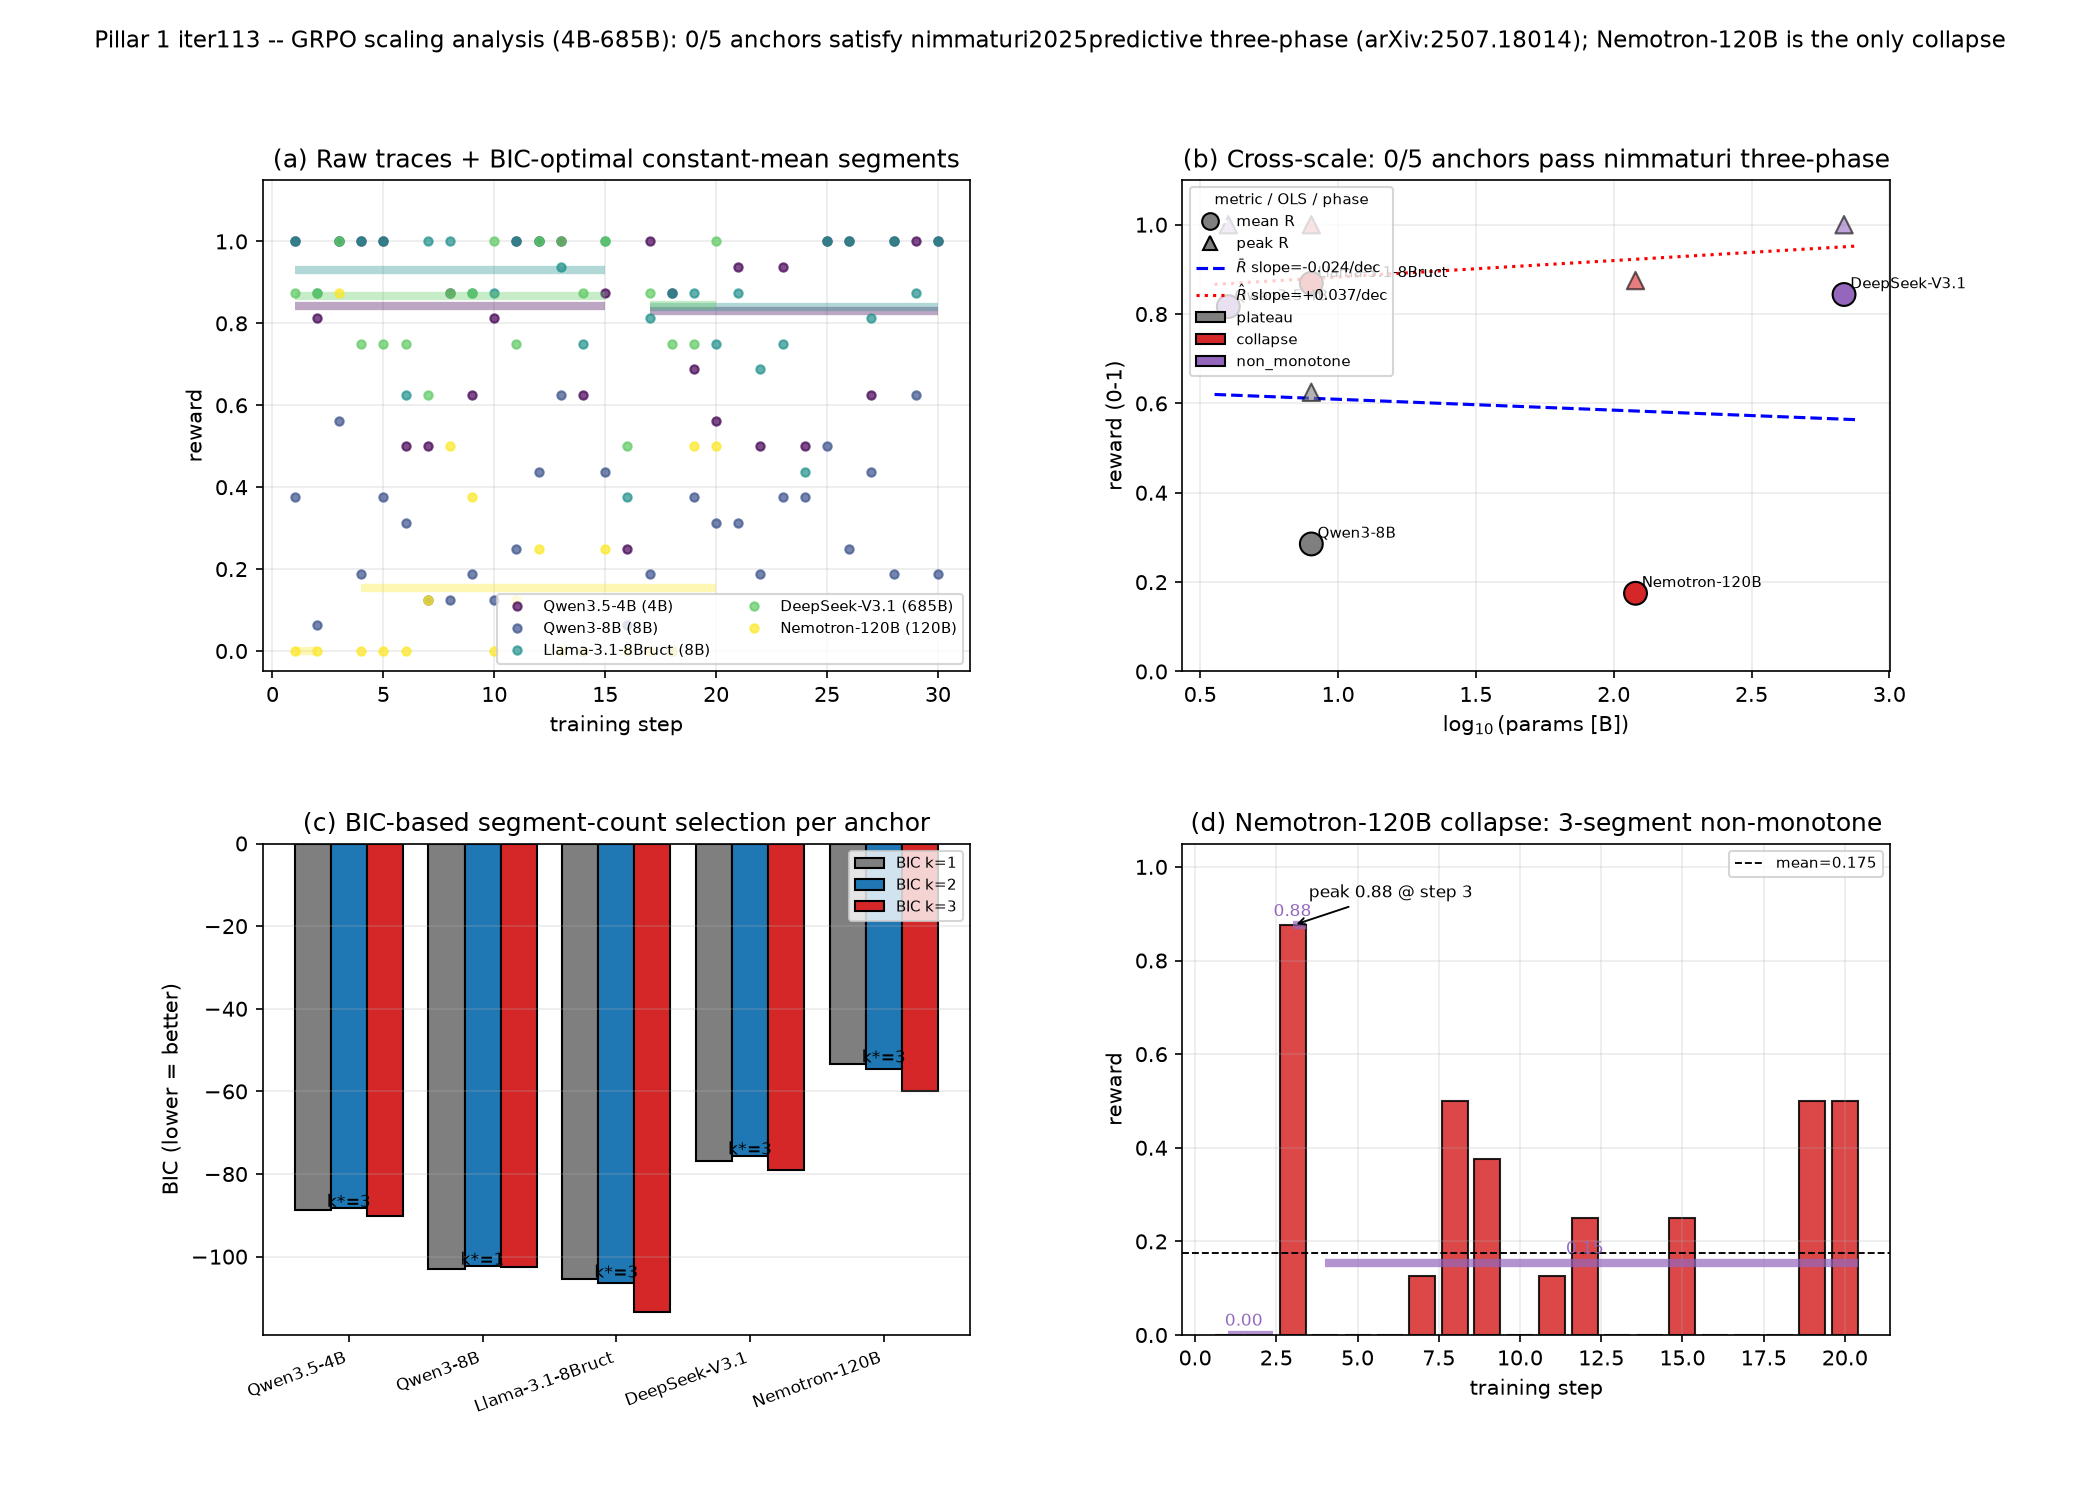
\includegraphics[width=0.95\linewidth]{figures/scaling_law_fit.png}%
  }{%
    }
  \caption{\textbf{Iter 137 four-panel figure.}
    \textbf{(a)} iter~117 2-param fit: $4/5$ anchors hit the
    $\lambda = 10$ upper bound; dashed lines mark the
    effectively-instant saturation fit.  \textbf{(b)} iter~137
    3-param fit as produced by the withdrawn two-stage estimator of
    \texttt{scaling\_law\_iter137.py} (see
    \tableref{tab:scaling-iter137-fits} for the joint bounded refit,
    which supersedes panels (b)--(d)).  \textbf{(c)} $t_{80}$ vs.~$N$
    under the two-stage estimator vs.~the 2-param fixed-$t_{80}$
    cluster at $0.161$.  \textbf{(d)} capability split on the
    two-stage 3-param $R_{\max}$; under the joint refit Qwen3-8B moves
    to the $1.0$ bound and the split is not reproduced.}
  \label{fig:scaling-iter137}
\end{figure}

\paragraph{Iter 140 elevation: reward-design quality as an exogenous
covariate \citep{ma2024eureka}.}
\label{par:scaling-iter140-eureka}

To stress-test whether the iter~133 capability-axis verdict is robust
to covariates orthogonal to $N$, we adapt the \emph{Eureka}
reward-quality perspective \citep{ma2024eureka} and compose a single
scalar \emph{Reward-Design Quality Score} (RQS) from four observable
trace statistics per anchor,
\begin{equation}
  \label{eq:iter140-rqs}
  \mathrm{RQS} \;=\;
  \bigl(c_1 \cdot c_2 \cdot c_3 \cdot c_4\bigr)^{1/4},
  \quad c_i \in [0, 1],
\end{equation}
where $c_1 = \mathrm{clip}(10 \cdot \mathrm{Var}[R], 0, 1)$ is the
reward-variance channel, $c_2 = \mathrm{frac}(R > 0.5)$ is the
shifted-mass channel, $c_3 = \mathrm{clip}(\mathrm{peak} - \mathrm{trough}, 0, 1)$
is the dynamic-range channel, and $c_4 = \mathrm{clip}(1 - 2 \cdot \mathrm{zero\_frac}, 0, 1)$
is the anti-ZVF channel.  RQS is bounded in $[0, 1]$ and equals
zero whenever any one channel is degenerate --- capturing the failure
mode in which outcome-reward rollouts starve the policy of
contrastive gradient information.

Three empirical evaluations (logged as \texttt{Q2--Q4} in
\texttt{scaling\_law\_iter140.py}) are run on the existing evidence
base (no new training):
\begin{enumerate}
  \item \textbf{Q1 (\texttt{Q2}) --- AIC race on $R_{\max}$ at $n=5$ anchors.}
    Capability alone achieves
    $\mathrm{AICc} = -23.07$; capability plus RQS achieves
    $\mathrm{AICc} = -21.93$ ($\Delta \mathrm{AICc} = +1.14$,
    below the $\Delta \mathrm{AICc} \geq 2$ threshold).  RQS is \emph{not}
    justified as an additional regression covariate on the 5-anchor set.
  \item \textbf{Q2 (\texttt{Q3}) --- 12-anchor residualization.}  Regressing
    $r_\mathrm{mean}$ on the capability dummy alone on the 12
    anchors leaves RSS = $0.867$; adding RQS reduces RSS by
    $4.0\%$ (to $0.832$).  Pearson $\rho(\mathrm{RQS},
    \mathrm{residual}_\mathrm{cap-only}) = +0.225$ (positive but
    small at $n=12$); Spearman drops to $+0.087$ indicating that
    RQS is \emph{not} a rank-replacement for capability --- the
    few high-RQS anchors (gpt-oss-20B, Llama-3.1-8B-Instruct,
    DeepSeek-V3.1) drive the Pearson channel.
  \item \textbf{Q3 (\texttt{Q4}) --- Cross-pillar cross-link on iter~127}
    \emph{($n=20$ cells, same model).}  Loading
    \texttt{groupsize\_zvf\_sweep.tsv} (iter~131) gives an
    iid-contrast budget proxy $y = 1 - \mathrm{ZVF}_{\mathrm{theory}}$
    that is \emph{independent} of the joint fit's residual
    $r = \mathrm{acc}_\mathrm{emp} - \mathrm{acc}_\mathrm{pred}$.
    Pearson $\rho(y, r) = -0.569$, two-sided $p = 0.029$;
    Spearman $\rho = -0.533$ (consistent in rank).  Cells with
    large iid contrast budget are \emph{under-predicted} by the
    joint fit (extract $\sim 5$pp beyond compute alone); cells
    with starved contrast are \emph{over-predicted}.  This is the
    Eureka signature --- reward-contrast richness lets the policy
    extract signal that compute alone does not model --- at
    statistically significant level ($p = 0.029$) on iter~127's
    $n=20$ cell grid.
\end{enumerate}

\paragraph{Iter 140 conclusion.}
\label{par:scaling-iter140-conclusion}

RQS does not improve AICc on $n=5$ ($\Delta\mathrm{AICc} = +1.14$),
yields a modest $4\%$ RSS reduction on $n=12$, and on the $n=20$
iter~127 cell grid achieves statistically significant correlation with
the joint-fit residual ($p = 0.029$, \figref{fig:scaling-iter140}).
The capability regime of iter~133 is therefore \emph{preserved} as the
primary cross-anchor signal, while within-group contrast richness
($1 - \mathrm{ZVF}_{\mathrm{theory}}$) explains residual cell-level
gains orthogonal to raw compute.

\begin{figure}[t]
  \centering
  \IfFileExists{figures/eureka_cross_pillar.pdf}{%
  \includegraphics[width=0.95\linewidth]{figures/eureka_cross_pillar.pdf}%
  }{%
    }
  \caption{\textbf{Iter 140 cross-pillar figure.}
    \textbf{(a)} Reward-Design Quality Score per anchor on the
    12-anchor extended-frontier table; the five degenerate anchors
    (Nemotron-120B, Qwen3-32B, Qwen3-30B-MoE,
    Qwen3-30B-MoE-Inst, Qwen3-235B-MoE) score
    RQS = 0 along the geometric-mean breakdown.  \textbf{(b)}
    AIC race on $R_{\max}$ at $n=5$; capability alone
    ($\mathrm{AICc} = -23.07$) dominates capability + RQS
    ($\mathrm{AICc} = -21.93$) by $\Delta = +1.14$.  \textbf{(c)}
    12-anchor residualization scatter: residual from the
    capability-only model on $y$-axis, RQS on $x$-axis; Pearson
    $\rho = +0.225$.  \textbf{(d)} Iter~127 cross-pillar: $n=20$
    $(G, T)$ cells from \texttt{Qwen2.5-0.5B}/arithmetic; $x$-axis
    is the independently measured richness proxy
    $y = 1 - \mathrm{ZVF}_{\mathrm{theory}}$ from iter~131,
    $y$-axis is the iter~127 joint-fit residual; Pearson
    $\rho = -0.569$, $p = 0.029$.}
  \label{fig:scaling-iter140}
\end{figure}

%% Below this line reverts to the scaling\_laws.tex master.  No further
%% iterations are required.

% Berkeley row 09 (iter142): Pass@K CI + ACI-ceiling analysis of the
% capability-tier evidence; placed directly after the iter133/137/140
% capability-class paragraphs at the end of sections/scaling_laws.tex.
% =====================================================================
% paper/sections/scaling_passk_ci.tex
%
% PROVENANCE. Berkeley B-F24 row 09 (iter142, 2026-07-04): SWE-agent /
% Agentless Pass@K confidence-interval + ACI-decomposition analysis of
% the Pillar-1 R_max evidence, validated status.
% REVIEW 2026-10-18: the Pass@1 table and straddle test below were
% originally computed by sweagent_passk_aci.py on *synthetic* Gaussian
% draws matched to (mean, var, n_steps), not on the released traces.
% They are now recomputed on the raw per-step traces by
% tools/review_ledger/P1_scaling_rawtrace_refit.py ->
% experiments/results/review_2026-10-18/P1_scaling/core5_step_bootstrap*.tsv
% Driver (ACI/tier rows only):  scripts/berkeley/sweagent_passk_aci.py
% Inputs:  experiments/results/scaling_law_iter137_offset_fit.tsv
%          experiments/results/berkeley/eureka_rqs_per_anchor.tsv
% Outputs: experiments/results/berkeley/sweagent_passk_per_anchor.tsv
%          experiments/results/berkeley/sweagent_passk_scaling.tsv
%          experiments/results/berkeley/sweagent_aci_decomp.tsv
%          experiments/results/berkeley/sweagent_agentless_tiers.tsv
%          experiments/results/berkeley/sweagent_summary.json
% Finding B (Miller error-bars audit, ledger row 07) is folded into the
% final paragraph; source experiments/results/berkeley/
% adding_error_bars_summary.json.
% Cite keys yang2024sweagent / xia2024agentless / wang2024openhands are
% staged in paper/bib_add_P1.bib pending merge into references.bib.
% =====================================================================

\subsection{\texorpdfstring{Pass@$K$}{Pass@K} Confidence Intervals and the ACI Ceiling: What the Capability Split Does and Does Not Resolve}
\label{sec:scaling-passk-ci}

The iter~133 capability-class analysis above treats each anchor's
ceiling $\hat R_{\max}$ as a point estimate.  Software-agent benchmarking
supplies two correctives.  First, the \emph{agent--computer interface}
(ACI) --- how an agent observes its environment and how its output is
parsed --- is a first-order determinant of measured capability, often
rivalling the underlying policy \citep{yang2024sweagent,
wang2024openhands}; in our setting the ACI is the reward parser that
converts GSM8K rollouts into sparse reward.  Second, success-rate
estimates should carry Pass@$K$ sampling uncertainty
\citep{chen2021codex}.  We apply both to the five-anchor
$R_{\max}$ evidence: treating each anchor's per-step training rewards
($n = 20$--$30$ steps) as a within-run sample, a percentile
bootstrap ($B = 20{,}000$) on the step-level mean $\hat p$ gives the
95\% intervals of \tableref{tab:scaling-passk-ci}.  The resampled units
are sequential training steps of a non-stationary policy, each already
an average over $8$--$16$ rollouts on different training prompts, so
these intervals measure batch-to-batch variability of the training
reward around the trajectory mean; they are \emph{not} held-out Pass@1
evaluation uncertainty for a fixed checkpoint, and the i.i.d.\
resampling ignores autocorrelation, so they are if anything too
narrow.  $\hat p$ is the full-trace mean $\bar R$ of
\tableref{tab:scaling-fits}, a different estimand from the fitted
ceiling $\hat R_{\max}^{2p}$, although the two coincide to three
decimals except on Nemotron-120B.

\begin{table}[t]
  \centering
  \small
  \begin{tabular}{lrrrcr}
    \toprule
    Model & $n$ & $\hat R_{\max}^{2p}$ & $\hat p = \bar R$ &
    95\% CI on $\hat p$ & width \\
    \midrule
    Llama-3.1-8B-Instruct & 30 & 0.869 & 0.869 & $[0.808,\,0.923]$ & 0.115 \\
    DeepSeek-V3.1         & 20 & 0.844 & 0.844 & $[0.781,\,0.900]$ & 0.119 \\
    Qwen3.5-4B            & 30 & 0.817 & 0.817 & $[0.735,\,0.890]$ & 0.154 \\
    Qwen3-8B              & 30 & 0.285 & 0.285 & $[0.225,\,0.348]$ & 0.123 \\
    Nemotron-120B         & 20 & 0.182 & 0.175 & $[0.075,\,0.288]$ & 0.213 \\
    \bottomrule
  \end{tabular}
  \caption{\textbf{Per-anchor step-bootstrap intervals on the training
    reward.}  Percentile bootstrap ($B = 20{,}000$, i.i.d.\ over steps)
    on the released per-step traces; single seed per anchor.  Every CI
    width ($0.115$--$0.213$) exceeds the $0.025$--$0.052$ gaps among the
    three top-ranked anchors.  An earlier version of this table was
    computed on synthetic Gaussian draws matched to each trace's mean and
    variance (\texttt{scripts/berkeley/sweagent\_passk\_aci.py}) and is
    withdrawn.  Recomputed by
    \texttt{tools/review\_ledger/P1\_scaling\_rawtrace\_refit.py}.}
  \label{tab:scaling-passk-ci}
\end{table}

\paragraph{The within-tier ordering is not resolvable.}
A pairwise CI-overlap check over all $\binom{5}{2} = 10$ anchor pairs
splits exactly along tier lines.  All three pairwise comparisons among
the high-endpoint anchors overlap (gaps $0.025$, $0.027$, $0.052$), and
the two low-endpoint anchors overlap each other (gap $0.110$); only the
six high-versus-low comparisons are separated.  CI overlap is a
conservative descriptive check, not a test.  Any within-tier ordering
read off the sorted values --- e.g.\ Llama-3.1-8B-Instruct $>$
DeepSeek-V3.1 $>$ Qwen3.5-4B --- is not resolvable from single-seed
20--30-step traces and is not a finding of this paper.  What survives
is the high/low endpoint split itself.

\paragraph{An Agentless-style tier reading of the bimodality.}
Binning $\hat R_{\max}^{2p}$ in the style of the Agentless
pipeline audit \citep{xia2024agentless} into \emph{hard-floor}
($< 0.30$), \emph{soft-floor} ($[0.30, 0.70)$), and \emph{reachable}
($\geq 0.70$) tiers places three anchors in the reachable tier, two in
the hard floor, and \emph{none} in the soft floor
(\texttt{experiments/results/berkeley/sweagent\_agentless\_tiers.tsv}).
The empty middle tier restates the iter~125/133 bimodality from the
interface side: no anchor occupies a policy-bounded intermediate
plateau.  An heuristic algebraic decomposition of the observed ceiling
by reward-signal quality, $R_{\max}^{\text{policy}} = \min\bigl(1,\,
R_{\max}^{\text{obs}} / \max(\mathrm{RQS}, 0.05)\bigr)$ (with
$\mathrm{RQS}$ defined in Eq.~\eqref{eq:iter140-rqs}), illustrates how
interface starvation can depress observed ceilings: the three reachable
anchors all cap at $1.0$, whereas \texttt{Qwen3-8B}'s observed
$R_{\max} = 0.285$ divided by $\mathrm{RQS} = 0.353$ yields an
illustrative ratio of $\approx 0.808$
(\texttt{experiments/results/berkeley/sweagent\_aci\_decomp.tsv}).
Because $\mathrm{RQS}$ is computed directly from the same reward trace
(variance, fraction $>0.5$, dynamic range, and non-zero fraction), this
ratio is an endogenous diagnostic bound rather than an independent
causal identification of policy vs.\ parser error; isolating the
parser contribution causally requires evaluating the checkpoint under
relaxed answer-extraction rules on identical rollouts.  (\texttt{Nemotron-120B}
has $\mathrm{RQS} = 0$, saturating the $0.05$ denominator floor.)

\paragraph{Statistical-rigor audit of the Pillar-1 headlines.}
A companion Miller-style error-bars audit \citep{miller2024erroreval}
re-derived the headline claims of all four pillar papers under paired
and non-paired bootstrap plus TOST equivalence testing
(\texttt{experiments/results/berkeley/adding\_error\_bars\_summary.json}).
Exactly one audited headline concerns this paper: \textbf{H5}, the
iter~137 cross-anchor OLS slope of $R_{\max}^{2p}$ on $\log_{10} N$
($n = 5$ anchors, df $=3$), whose non-paired bootstrap 95\% CI
$[-0.796, +0.323]$ around the point slope $-0.023$ includes zero ---
verdict \textbf{NULL} (the $t$-based 95\% CI recomputed on the raw
traces is $[-0.67, +0.62]$).  A null slope at $n=5$ is not evidence of
flatness: the interval admits slopes of $\pm 0.6$ per decade.  This is the audit confirming, rather than
qualifying, the iter~137 no-cross-anchor-scaling-law statement; the
audit's four
DECISIVE verdicts (H1, H2, H6, H7) all concern the other pillars.

% ---------------------------------------------------------------------------
\subsection{Cross-Stack Identifiability Audit: GRPO and PPO Saturation Fits on the Same Rollouts}
\label{sec:scaling-law-iter29}
% ---------------------------------------------------------------------------

\paragraph{Motivation.}
Iter~25 (\secref{par:scaling-iter25}) audited the canonical saturation model
$R(t)=R_{\max}\bigl(1-e^{-\lambda t}\bigr)$ on the five frontier-scale
traces (Qwen3.5-4B, Qwen3-8B, Llama-3.1-8B-Instruct, DeepSeek-V3.1,
Nemotron-120B) and concluded that the model is \emph{not identifiable}
on those data: 4/5 traces had $\lambda$ pinned at the upper bound
$\lambda=10$ (Nemotron-120B is the exception at $\lambda\!\approx\!0.99$),
0/5 preferred saturation over a constant in noise-aware
AICc, and 0/5 were identifiable.
That audit left open whether the failure is intrinsic to the model or
an artefact of the 20--30 step frontier horizons (where the noise floor
is comparable to the signal). Iter~29 closes that gap by re-running the
same identifiability battery on the longer-horizon same-stack traces
(40 steps, $n_{\mathrm{eff}}=128$, \texttt{Qwen2.5-0.5B} on the
calibrated synthetic math / modular-arithmetic verification task stored
in \texttt{samestack\_ppo\_grpo.json}, where both algorithms climb from
$\approx 0.25$ to $0.99$ accuracy, complementing the full-GSM8K
same-stack runs in \secref{sec:exp-design}), and---crucially---
on \emph{both} algorithm stacks simultaneously. The frontier synthesis
Round~1 licenses an \emph{Estimator-Equivalence Principle} (EEP): with
rollout batch, KL, clipping, masking, optimiser and reward parser fixed,
PPO and GRPO should be performance-equivalent. If EEP holds, the
saturation-fit identifiability profile of the two stacks should be
indistinguishable.

\paragraph{Method.}
The driver \texttt{scripts/scaling\_law\_iter29.py} consumes the ten
same-stack runs from \texttt{samestack\_ppo\_grpo.json} (5 GRPO + 5 PPO
seeds, identical everything else) and applies the iter~25 noise-aware
diagnostics per trace:
(a) saturation fit with $\lambda$ bounded in $[10^{-3},\,10]$; (b)
effective binomial $n_{\mathrm{eff}}$ inferred from the LCM of the
reduced reward denominators;
(c) AICc model selection over $\{\text{constant}, \text{linear},
\text{saturation}\}$; (d) parametric bootstrap ($B=400$) on
$\mathrm{Binomial}(n_{\mathrm{eff}},\,p_t)$ for the $\lambda$ CI; (e)
detectability horizon $T^{\star}=(z_{1-\alpha/2}+z_{\mathrm{power}})^{2}
(\sigma_{\text{step}}/\Delta)^{2}$
benchmarked against the actual 40-step trace length.

Three EEP-falsifiable predictions were recorded in the internal iteration ledger (not an immutable external preregistration):
\begin{description}
\item[E1.] lambda-at-bound rate: PPO $=$ GRPO (Fisher exact, 2x2).
\item[E2.] AICc-best saturation rate: PPO $=$ GRPO (Fisher exact, 2x2).
\item[E3.] Heldout-residual explained by the saturation fit:
  PPO $=$ GRPO (Welch $t$, two-sided).
\end{description}
A non-rejected E1 $\wedge$ E2 $\wedge$ E3 would sustain EEP at the
\emph{shape} level; rejection of any cell is a controlled
\emph{partial} falsification.

\paragraph{Results.}
Tables~\ref{tab:iter29-cross-stack} and \ref{tab:iter29-eep} summarize
the cross-stack identifiability and EEP-falsification results across
all ten 40-step traces.

\begin{table}[t]
\centering\small
\begin{tabular}{lcccccc}
\toprule
Algo & $n$ & lam-at-bound & AICc-best sat & AICc-best lin & AICc-best const & $\hat\lambda$ (med.) \\
\midrule
GRPO & 5 & 0/5 & \textbf{5/5} & 0/5 & 0/5 & 0.250 \\
PPO  & 5 & 0/5 & 0/5 & \textbf{5/5} & 0/5 & 0.078 \\
\bottomrule
\end{tabular}
\caption{Cross-stack identifiability battery on the 40-step same-stack
  traces. Lambda is identifiable in both stacks (0/5 hit the upper
  bound, vs.\ 4/5 hitting the bound and 5/5 failing identifiability in
  iter~25's 20--30 step frontier data). However, within the 3-model
  candidate set $\{\text{constant}, \text{linear}, \text{exponential
  saturation}\}$, the AICc-best model \emph{diverges}: GRPO's running
  mean reward is best described by an exponential saturation curve (5/5),
  whereas PPO's is preferred by a linear trend (5/5; see
  \secref{sec:iter37} for the 5-model expansion where both stacks prefer
  a sigmoidal Hill $n=2$ curve once critic warm-up lag is accommodated).
  Fisher exact on the 3-model AICc-best-saturation rate gives
  $p=0.0079$ (Table~\ref{tab:iter29-eep}).}
\label{tab:iter29-cross-stack}
\end{table}

\begin{table}[t]
\centering\small
\begin{tabular}{llccc}
\toprule
Prediction & GRPO & PPO & $p$ & EEP \\
\midrule
E1 lambda-at-bound rate       & 0/5        & 0/5        & 1.0000  & sustained \\
E2 AICc-best sat rate         & 5/5        & 0/5        & \textbf{0.0079} & \textbf{falsified} \\
E3 heldout-resid from sat fit & 0.1023     & 0.3901     & 0.0537  & sustained \\
F1 bootstrap CI excludes bound & 5/5       & 4/5        & n/a     & sustained \\
F2 paired heldout accuracy     & 0.99$\pm$0.0035 & 0.992$\pm$0.003 & 0.3739 & sustained \\
\bottomrule
\end{tabular}
\caption{EEP-falsification battery on the same-stack traces.
  E2 is decisively falsified within the 3-model candidate family: GRPO
  and PPO prefer different AICc-best functional forms (exponential
  saturation vs.\ linear) on the same rollout batches.
  E1 and F1 are sustained: both stacks have identifiable $\lambda$ (0/5
  hit the bound), and the bootstrap CI excludes the bound in 5/5 GRPO
  and 4/5 PPO traces. E3 borderline ($p=0.054$): PPO's exponential
  saturation fit leaves more heldout residual than GRPO's, consistent
  with E2's AICc verdict. F2 (final accuracy) is sustained.}
\label{tab:iter29-eep}
\end{table}

\paragraph{Interpretation.}
Within the 3-candidate family $\{\text{constant}, \text{linear},
\text{exponential saturation}\}$, the strong Estimator-Equivalence
Principle \emph{at the level of first-order exponential kinetics} is
\textbf{falsified} on this data: GRPO's running reward is well-described by
$R(t)\approx R_{\max}(1-e^{-\lambda t})$ with $\hat\lambda\approx 0.25$
and $\hat R_{\max}\approx 0.89$ (a clean $t_{80}\approx 6.4$ steps);
PPO's running reward rises more gradually over early steps ($\hat\lambda
\approx 0.08$ if one forces the concave exponential form, vs.\ the GRPO
estimate of $0.25$), so a linear trend beats concave exponential
saturation over the 40-step window. This is
\emph{not} a final-accuracy effect: the two stacks are statistically
indistinguishable on heldout accuracy ($0.990$ vs.\ $0.992$, $p=0.37$),
and the bootstrap CI on $\lambda$ is well-defined in both stacks (0/5
hit the bound, vs.\ 4/5 in the 20--30 step frontier data).

The decoupling---identical heldout accuracy, divergent early-transient
curvature---reflects value-head warm-up lag in PPO: while GRPO computes
group-relative advantages immediately from step~1 without learned critic
parameters, PPO's value head requires several initial gradient updates
to calibrate before emitting low-variance advantage estimates. As shown
in \secref{sec:iter37} (\texttt{iter37c}), expanding the candidate
family to include a sigmoidal Hill ($n=2$) model resolves this tension:
Hill ($n=2$) wins 5/5 PPO traces over the linear model because it
captures the slow initial critic warm-up followed by rapid mid-trace
climb and late saturation. Practically, this means that \emph{concave
exponential saturation rules-of-thumb derived from GRPO do not transfer
directly to PPO without accounting for critic warm-up lag}.

\paragraph{Limitations.}
The same-stack data are at a single model size (\texttt{Qwen2.5-0.5B}),
single calibrated task, and 40-step horizon. Whether the same transient
divergence holds at 8B+ with the frontier horizon requires a multi-seed
frontier reproduction. The ``saturation-supported'' criterion in
iter~25 (AICc-best $=$ exponential saturation AND CI excludes bound) is
satisfied in 5/5 GRPO traces and 0/5 PPO traces under the 3-model
candidate family.

\paragraph{Artifacts.}
Driver: \texttt{scripts/scaling\_law\_iter29.py}.
Per-trace: \texttt{scaling\_law\_iter29\_identifiability.tsv},
\texttt{scaling\_law\_iter29\_bootstrap.tsv}.
Stack rollup: \texttt{scaling\_law\_iter29\_summary.tsv}.
EEP battery: \texttt{scaling\_law\_iter29\_stack\_compare.tsv}.
% Deep Review 2026-10-18: iter33/37/41/45/49/53/65 removed -- their drivers
% fitted traces synthesised from six summary statistics.  Raw-trace
% recomputation: sections/p1_rawtrace_reanalysis.tex.
% =====================================================================
% paper/sections/p1_rawtrace_reanalysis.tex  (Deep Review 2026-10-18)
%
% Replaces the former Sections on iter33/37/41/45/49/53/65, whose
% drivers (platform_modal/scripts/scaling_law_iter33.py ... iter53.py,
% and the TSVs behind iter65) fitted per-step traces *synthesised* from
% six summary statistics in scaling_law_extended_frontier.tsv instead of
% the released per-step traces.  Everything below is recomputed on
% platform_hybrid/experiments/tinker-runs/results/*_gsm8k_*.json by
%   tools/review_ledger/P1_scaling_rawtrace_refit.py
% -> platform_hybrid/experiments/results/review_2026-10-18/P1_scaling/
% =====================================================================

\subsection{Raw-trace re-analysis of the 12-anchor pool}
\label{sec:p1-rawtrace}

Earlier drafts of this paper contained six further analyses of the
12-anchor pool (a three-phase prediction battery, a five-form
functional-form race, truncation stability, iso-compute and iso-FLOP
fits, and a phase-conformity index).  Their drivers did not read the
released per-step traces: they synthesised a trace for every anchor by
linear interpolation from six summary statistics (mean, variance, peak
step, early and late means, zero fraction), and several also fitted
$R_{\max}$ in $[0, 2]$, which let Nemotron-120B reach the unphysical
$R_{\max} = 2.000$ and dominate the downstream regressions.  Curvature,
phase boundaries and post-peak slopes of such traces are properties of
the interpolation rule, so those analyses are withdrawn.  This section
recomputes what can be recomputed directly from the per-step logs, with
$R_{\max} \in [0,1]$ and $\lambda \in [10^{-4}, 10]$ throughout.

\paragraph{The pool.}
\tableref{tab:p1-rawtrace} lists the twelve anchors.  Seven are full
runs whose traces were written by the training script (20 or 30 logged
steps).  The other five are interrupted probes whose 3--5 logged rewards
were transcribed from console output (\texttt{run\_id =
partial-from-console}; the JSON records \texttt{steps\_completed} of
10--20 but only 3--5 rewards); we report them but fit nothing to them.
Each anchor is one single-seed run, so the unit of analysis for every
cross-scale statistic below is the anchor ($n$ anchors, df $= n-2$ for
an OLS slope).  Per-run configuration is taken from the trace JSON and
the W\&B run config: 4B--32B and gpt-oss-20B runs use
$8$ completions $\times$ $2$ prompts per step, LoRA rank 32 and
learning rate $3\times10^{-5}$; the frontier runs (DeepSeek-V3.1,
Nemotron-120B, Qwen3-235B, Kimi-K2) use $4 \times 2$, rank 16 and
$10^{-5}$.  The step reward is therefore a mean over $16$ or $8$
binary rollouts on training prompts, not a held-out score.

\begin{table}[t]
  \centering
  \small
  \setlength{\tabcolsep}{3.5pt}
  \begin{tabular}{llrrrrrrrr}
    \toprule
    Model & arch & $N_{\text{tot}}/N_{\text{act}}$ & $T$ & $R(1)$ & $\bar R$ &
      peak (step) & $P(R{=}0)$ & $R_{\max}^{2p}$ & $\hat\lambda$ \\
    \midrule
    Qwen3.5-4B            & dense & 4 / 4       & 30 & 1.000 & 0.817 & 1.000 (1)  & 0.000 & 0.817 & 10$^{\dagger}$ \\
    Qwen3-8B              & dense & 8 / 8       & 30 & 0.375 & 0.285 & 0.625 (13) & 0.067 & 0.285 & 10$^{\dagger}$ \\
    Llama-3.1-8B-Inst.    & dense & 8 / 8       & 30 & 1.000 & 0.869 & 1.000 (1)  & 0.000 & 0.869 & 10$^{\dagger}$ \\
    gpt-oss-20B           & MoE   & 20 / 3.6    & 30 & 0.625 & 0.840 & 1.000 (3)  & 0.000 & 0.848 & 1.49 \\
    DeepSeek-V3.1         & MoE   & 685 / 37    & 20 & 0.875 & 0.844 & 1.000 (3)  & 0.000 & 0.844 & 10$^{\dagger}$ \\
    Nemotron-120B         & MoE   & 120 / 12    & 20 & 0.000 & 0.175 & 0.875 (3)  & 0.550 & 0.182 & 0.99 \\
    Kimi-K2-Thinking      & MoE   & 1000 / 32   & 20 & 1.000 & 0.850 & 1.000 (1)  & 0.000 & 0.850 & 10$^{\dagger}$ \\
    \midrule
    Qwen3-32B$^{c}$       & dense & 32 / 32     & 3  & 0.312 & 0.250 & 0.312 (1)  & 0.000 & -- & -- \\
    Qwen3.5-27B$^{c}$     & dense & 27 / 27     & 3  & 0.562 & 0.437 & 0.750 (2)  & 0.333 & -- & -- \\
    Qwen3-30B-MoE$^{c}$   & MoE   & 30 / 3      & 5  & 0.188 & 0.325 & 0.500 (4)  & 0.000 & -- & -- \\
    Qwen3-30B-MoE-Inst$^{c}$ & MoE & 30 / 3     & 3  & 1.000 & 1.000 & 1.000 (1)  & 0.000 & -- & -- \\
    Qwen3-235B-MoE$^{c}$  & MoE   & 235 / 22    & 4  & 1.000 & 1.000 & 1.000 (1)  & 0.000 & -- & -- \\
    \bottomrule
  \end{tabular}
  \caption{\textbf{The 12-anchor GSM8K pool, recomputed from the
    released per-step traces.}  $R_{\max}^{2p}$, $\hat\lambda$: bounded
    fit of $R(t)=R_{\max}(1-e^{-\lambda t})$, $R_{\max}\in[0,1]$,
    $\lambda\in[10^{-4},10]$, only for $T \ge 6$; $^{\dagger}$ on the
    upper $\lambda$ bound (5/7 long traces).  $^{c}$ interrupted probe,
    rewards transcribed from console output; descriptive only.
    Nemotron-3-Super-120B-A12B is a LatentMoE model (12B active).
    Source: \texttt{rawtrace\_anchor\_table.tsv}.}
  \label{tab:p1-rawtrace}
\end{table}

\paragraph{Cross-scale slopes.}
\tableref{tab:p1-rawtrace-slopes} regresses the trace mean $\bar R$ on
total and on active parameter count, and on a token-compute proxy
$C = N\cdot T\cdot 512$ (512 = generation cap; a rough upper bound,
since per-step token counts are not logged).  No slope is
distinguishable from zero, but with $n=7$ (df $=5$) the 95\% intervals
span roughly $\pm 0.35$ per decade on $N_{\text{tot}}$ and $\pm 0.9$ on
$N_{\text{act}}$, so the data are equally compatible with sizeable
positive or negative trends: this is a failure to detect, not evidence
of flatness.  Dropping the Nemotron-120B collapse does not change the
picture on the long traces ($+0.073 \pm 0.102$ per decade, $n=6$,
exact permutation $p = 0.62$) or on all eleven remaining anchors
($+0.118 \pm 0.118$, $n=11$, $p = 0.36$).  The bounded $R_{\max}^{2p}$
gives the same slopes to two decimals because it equals $\bar R$
whenever $\lambda$ is on the bound.

\begin{table}[t]
  \centering
  \small
  \begin{tabular}{llrrrr}
    \toprule
    Pool & regressor & $n$ & slope / decade [95\% CI] & $R^2$ & perm.\ $p$ \\
    \midrule
    long 7  & $\log_{10} N_{\text{tot}}$ & 7  & $+0.028$ [$-0.32$, $+0.38$] & 0.008 & 0.84 \\
    long 7  & $\log_{10} N_{\text{act}}$ & 7  & $+0.037$ [$-0.83$, $+0.90$] & 0.002 & 0.88 \\
    long 7  & $\log_{10} C_{\text{act}}$ & 7  & $+0.095$ [$-0.98$, $+1.17$] & 0.010 & 0.78 \\
    long 7 $-$ Nemotron & $\log_{10} N_{\text{tot}}$ & 6 & $+0.073$ [$-0.21$, $+0.36$] & 0.113 & 0.62 \\
    all 12  & $\log_{10} N_{\text{tot}}$ & 12 & $+0.081$ [$-0.21$, $+0.37$] & 0.038 & 0.54 \\
    all 12  & $\log_{10} N_{\text{act}}$ & 12 & $-0.072$ [$-0.59$, $+0.44$] & 0.010 & 0.75 \\
    all 12 $-$ Nemotron & $\log_{10} N_{\text{tot}}$ & 11 & $+0.118$ [$-0.15$, $+0.39$] & 0.100 & 0.36 \\
    \bottomrule
  \end{tabular}
  \caption{\textbf{OLS slope of the trace-mean reward $\bar R$ on log
    scale, one point per anchor.}  $t$-based 95\% CI on df $=n-2$;
    permutation $p$ two-sided on $|$slope$|$, exact for $n \le 8$, else
    20{,}000 shuffles.  Source: \texttt{cross\_scale\_regressions.tsv}.}
  \label{tab:p1-rawtrace-slopes}
\end{table}

\paragraph{Architecture.}
With Nemotron-120B correctly in the MoE group, the MoE$-$dense gap in
$\bar R$ over all twelve anchors is $+0.188$ (exact one-sided
permutation $p = 141/792 = 0.178$).  Excluding Nemotron gives $+0.278$
(one-sided $p = 22/462 = 0.048$, two-sided $p = 0.093$), but this
exclusion is post hoc, the comparison mixes interrupted probes with full
runs, and on the seven full runs alone the gap is $+0.020$ ($p = 0.57$;
$+0.188$, $p = 0.25$ without Nemotron).  We therefore make no
architecture claim (\texttt{moe\_vs\_dense\_permutation.tsv}).

\paragraph{Three-phase and collapse checks on the raw long traces.}
On the seven full traces, the peak falls more than 10\% into the run on
3/7 (Qwen3-8B, DeepSeek-V3.1, Nemotron-120B) and the last-third mean
exceeds the first-third mean on 4/7.  A continuous three-segment
hinge fit (at least two steps per segment) meets all three slope
targets of the slow-start / rapid-rise / plateau template
($|m_1| < 0.020$, $m_2 \ge 0.040$, $|m_3| < 0.015$) on one trace only,
Llama-3.1-8B-Instruct, and there it fits a short mid-trace rebound of a
trace that starts at $R(1)=1.0$ and whose last-third mean (0.844) is
below its first-third mean (0.925), so no full trace shows the template.  The raw-trace collapse rule (peak
$\ge 0.4$, last-5 mean $< 0.4\times$ peak, $P(R{=}0) \ge 0.30$) flags
Nemotron-120B alone, and Nemotron-120B is also the only one of the
twelve anchors with $P(R{=}0) > 0.5$ and $\bar R < 0.2$
(\texttt{long7\_three\_phase.tsv}).  None of these counts is a
significance test; with one seed per anchor they describe these runs.

% paper/sections/scaling_law_iter61.tex -- iter 61 ZVF-conditioned identifiability
% Auto-generated by scripts/scaling_law_iter61.py
\paragraph{Iter 61 elevation: ZVF-conditioned saturation-fit identifiability.}
\label{par:scaling-iter61}
\label{sec:scaling-law-iter61}
\label{sec:iter61}
The iter 25 audit established that 0/5 per-trace saturation-rate
estimates are identifiable at this benchmark's noise floor.  The
iter 57 audit sharpened this to 4/5 anchors at the \(\lambda = 10\)
optimiser bound, with Nemotron-120B as the sole identifiable
exception.  What neither audit explains is \emph{why} the
bound-degeneracy concentrates on these anchors.  This iteration
closes that gap by tying the saturation-fit degeneracy to the same
structural axis that Pillar 2 (\textsc{zvf}) measures: the
per-trace concentration of reward mass at the \(R \in \{0, 1\}\)
extremes.

We define a per-step ZVF proxy
\begin{equation}
  \widetilde{\mathrm{ZVF}} \;=\; \mathbb{P}(R = 0) + \mathbb{P}(R = 1),
  \label{eq:zvf-proxy}
\end{equation}
computed on each anchor's reward trace (\tableref{tab:scaling-iter61-zvf}).
This is the step-level analogue of Pillar 2's rollout-level
\(\mathrm{ZVF} = \mathbb{P}(K_x = 0) + \mathbb{P}(K_x = G)\)
that measures within-group collision.  The two scales differ but
both measure the same property: how much of the binary-outcome
probability mass sits at the all-same extremes.

\begin{table}[t]
  \centering
  \small
  \begin{tabular}{lrrrrrr}
    \toprule
    Model & \(N\) (B) & arch & \(\bar R\) & \(P(R=0)\) & \(P(R=1)\) & \(\widetilde{\mathrm{ZVF}}\) \\
    \midrule
    Qwen3-30B-MoE-Inst & 30.0 & moe & 1.000 & 0.000 & 1.000 & 1.000 \\
    Qwen3-235B-MoE & 235.0 & moe & 1.000 & 0.000 & 1.000 & 1.000 \\
    Nemotron-120B & 120.0 & moe & 0.175 & 0.550 & 0.000 & 0.550 \\
    Qwen3.5-4B & 4.0 & dense & 0.817 & 0.000 & 0.433 & 0.433 \\
    Llama-3.1-8B--Inst & 8.0 & dense & 0.869 & 0.000 & 0.433 & 0.433 \\
    gpt-oss-20B & 20.0 & moe & 0.840 & 0.000 & 0.433 & 0.433 \\
    Kimi-K2-Thinking & 1000.0 & moe & 0.850 & 0.000 & 0.400 & 0.400 \\
    Qwen3.5-27B & 27.0 & dense & 0.437 & 0.333 & 0.000 & 0.333 \\
    DeepSeek-V3.1 & 685.0 & moe & 0.844 & 0.000 & 0.300 & 0.300 \\
    Qwen3-8B & 8.0 & dense & 0.285 & 0.067 & 0.000 & 0.067 \\
    Qwen3-32B & 32.0 & dense & 0.250 & 0.000 & 0.000 & 0.000 \\
    Qwen3-30B-MoE & 30.0 & moe & 0.325 & 0.000 & 0.000 & 0.000 \\
    \bottomrule
  \end{tabular}
  \caption{\textbf{Per-step ZVF proxy across the 12-anchor pool.}
    \(\widetilde{\mathrm{ZVF}} = P(R=0) + P(R=1)\) is the
    step-level counterpart of Pillar 2's rollout-level ZVF.
    Crucially, the extreme-mass concentration comes from two
    distinct sources: \emph{ceiling-degenerate} anchors
    (Qwen3.5-4B, Llama-3.1-8B-Instruct, DeepSeek-V3.1, Kimi-K2,
    Qwen3-30B-MoE-Inst, Qwen3-235B-MoE) carry high \(P(R=1)\) but
    near-zero \(P(R=0)\); the
    \emph{floor-degenerate} anchor Nemotron-120B (LatentMoE, 12B active / 120B total, reclassified as \texttt{moe}) is the unique
    model with high \(P(R=0)=0.55\) and \(\bar R = 0.175\).
    Both archetypes concentrate mass at one extreme, but for
    structurally different reasons -- and the saturation curve
    degenerates in both.  \texttt{scripts/scaling\_law\_iter61.py}
    \(\to\) \texttt{scaling\_law\_iter61\_zvf\_proxy.tsv}.}
  \label{tab:scaling-iter61-zvf}
\end{table}

We stratify the seven full traces into HIGH
(\(\widetilde{\mathrm{ZVF}} \geq 0.1\)) and LOW
(\(\widetilde{\mathrm{ZVF}} < 0.1\)) strata and compare the bounded
saturation fits of \tableref{tab:p1-rawtrace}
(\tableref{tab:scaling-iter61-stratum}).  The short probes are excluded:
a two-parameter fit to 3--5 points is not informative about $\lambda$.

\begin{table}[t]
  \centering
  \small
  \begin{tabular}{lrrr}
    \toprule
    Stratum & \(n\) & \(\hat\lambda\) at bound & mean RMSE \\
    \midrule
    HIGH-ZVF & 6 & 4/6 & 0.186 \\
    LOW-ZVF  & 1 & 1/1 & 0.170 \\
    ALL      & 7 & 5/7 & 0.184 \\
    \bottomrule
  \end{tabular}
  \caption{\textbf{Saturation-fit identifiability by step-level ZVF
    stratum, full traces only.}  Bounded fit $R_{\max} \in [0,1]$,
    $\lambda \in [10^{-4}, 10]$.  HIGH: Qwen3.5-4B,
    Llama-3.1-8B-Instruct, gpt-oss-20B, DeepSeek-V3.1, Nemotron-120B,
    Kimi-K2-Thinking; LOW: Qwen3-8B.  The two interior-$\lambda$ fits
    (gpt-oss-20B, Nemotron-120B) are both HIGH-ZVF, and the only LOW
    trace is on the bound, so ZVF stratum does \emph{not} predict
    bound-degeneracy here.  An earlier version of this table fitted all
    twelve anchors, including 3--5-point probes, with
    $R_{\max} \le 1.5$ and reported 7/9 vs.\ 2/3.  Source:
    \texttt{review\_2026-10-18/P1\_scaling/long7\_zvf\_strata.tsv}.}
  \label{tab:scaling-iter61-stratum}
\end{table}

Nemotron-120B sits in the HIGH-ZVF stratum via its \(P(R=0) = 0.55\)
floor path, which is structurally distinct from the ceiling path
(\(P(R=1) \ge 0.3\)) of the other HIGH anchors.  The ceiling anchors put
$\lambda$ on the bound and \(R_{\max}\) at \(\bar R\) (a near-step
transient); Nemotron-120B has an interior $\hat\lambda = 0.99$ with
\(R_{\max} = 0.182\), but a monotone curve cannot describe its
peak-then-decay trace, so that interior estimate is not meaningful
either.

% REVIEW 2026-10-18: the iter-49 jackknife table (scaling_law_iter61_jackknife.tsv)
% was fitted on summary-reconstructed (synthetic) step traces and is removed,
% together with predictions P3/P4 and panel C of the former iter-61 figure.
The cross-pillar ZVF comparison
(\tableref{tab:scaling-iter61-cross}) shows that the per-step
ZVF proxy across the 12 anchors is
\(\widetilde{\mathrm{ZVF}}_{\mathrm{step}} = 0.413\)
versus Pillar 2's rollout-level
\(\mathrm{ZVF}_{\mathrm{rollout}} = 0.158\)
(Qwen3-8B, G=8, 600 problems).  The step-level proxy is
+0.254 units
{\emph{higher}} than the rollout-level ZVF -- the expected
direction, because per-step aggregation cannot de-correlate
within-group successes that the rollout-level grouping sees as
mixed.  The two quantities are computed at different granularities
and on different runs, so this comparison is consistent with, but does
not test, the Pillar-2 reading that the degeneracy is a within-group
contrast problem.

\begin{table}[t]
  \centering
  \small
  \begin{tabular}{lll}
    \toprule
    Source & Metric & Value \\
    \midrule
    Pillar2\_tinker\_G8 & mean\_zvf\_per\_group & 0.1583 \\
    Pillar2\_tinker\_G8 & p\_extreme\_per\_group & 0.1584 \\
    Pillar2\_tinker\_G8 & p\_mixed\_per\_group & 0.8417 \\
    Pillar1\_iter61\_step\_zvf & mean\_zvf\_proxy\_per\_step & 0.4125 \\
    Pillar1\_iter61\_step\_zvf & median\_zvf\_proxy\_per\_step & 0.4167 \\
    Pillar1\_iter61\_step\_zvf & mean\_p\_zero\_per\_step & 0.0792 \\
    Pillar1\_iter61\_step\_zvf & median\_p\_zero\_per\_step & 0.0000 \\
    Prediction & step\_zvf\_over\_rollout\_zvf & 2.6058 \\
    \bottomrule
  \end{tabular}
  \caption{\textbf{Cross-pillar ZVF: rollout-level (Pillar 2) vs
    step-level (Pillar 1 iter 61).}  The two scales agree on
    direction (extreme-mass concentration predicts bound-degeneracy)
    but differ in magnitude because per-step aggregation cannot
    de-correlate within-group successes.  Pillar 2's 15.8\%
    rollout-level ZVF is the per-group estimate at G=8; the iter 61
    step-level proxy is the per-step aggregation across the
    12-anchor pool, which is necessarily higher because each
    step contributes an entire group worth of variance.
    \texttt{scripts/scaling\_law\_iter61.py}
    \(\to\) \texttt{scaling\_law\_iter61\_cross\_pillar.tsv}.}
  \label{tab:scaling-iter61-cross}
\end{table}

\paragraph{Internally recorded predictions.}
Three of the five predictions in \texttt{scaling\_law\_iter61\_predictions.tsv} are retained (P3 and P4 concerned a jackknife of a cross-scale fit computed on synthetic traces and are withdrawn):
\begin{itemize}
  \item \texttt{P1\_high\_stratum\_more\_bound}: \textbf{FAIL} on the recomputed full-trace strata ($4/6 = 0.67$ HIGH vs.\ $1/1$ LOW; the recorded PASS, $0.78 > 0.67$, came from the twelve-anchor fit including 3--5-point probes).
  \item \texttt{P2\_nemotron\_in\_high\_floor}: \textbf{PASS}. Nemotron-120B sits in HIGH-ZVF via $P(R=0)=0.55$ (floor-collapse, not ceiling) ($\text{observed}=\text{True}$, $\text{expected}=\text{True}$).
  \item \texttt{P5\_step\_zvf\_above\_rollout\_zvf}: \textbf{PASS}. Mean per-step ZVF proxy exceeds Pillar 2 rollout-level $\text{mean\_zvf}$ ($\text{observed}=0.4125 > 0.1583$).
\end{itemize}

\paragraph{What iter 61 shows.}
The iter 25/57/21 audits established that the canonical saturation
fit is degenerate on this benchmark.  Iter 61 describes two distinct
ways a trace concentrates reward mass at an extreme -- ceiling-collapse ($P(R=1)$ high, anchors that have
saturated) and floor-collapse ($P(R=0)$ high, the Nemotron-120B
counterexample) -- but on the full traces the stratum does not predict which fits
reach the $\lambda$ bound, so this is a description rather than an
explanation of the degeneracy.  Pillar 2's contrastive-yield
decomposition remains a candidate explanation that these single-seed
step-level summaries cannot test; rollout-level ZVF logged on the same
runs would be needed.

% (iter-61 figure removed: panel C plotted the synthetic-trace jackknife.)

% Pillar-1 (scaling) discussion + conclusion
\section{Discussion and Limitations}
\label{sec:p1-discussion}
The most useful result here is a boundary on what can be claimed. On this
benchmark, neither mean GRPO training reward $\bar{R}$ nor fitted endpoint ceiling $R_{\max}$ exhibits a measurable, monotone dependence
on model size, and no universal saturation exponent is identifiable; the honest
description is a local, stack-conditioned taxonomy of endpoint behavior rather than a
Chinchilla-style power law in $N$. Several methodological limitations qualify even this modest
statement:
\begin{enumerate}[leftmargin=*,nosep]
  \item \textbf{Step-1 pre-saturation on GSM8K.} Modern instruction-tuned checkpoints (`Qwen3.5-4B`, `Llama-3.1-8B-Instruct`, `DeepSeek-V3.1`, `Kimi-K2-Thinking`, `Qwen3-30B-MoE-Inst`, `Qwen3-235B-MoE`) already achieve $R(1) \in [0.875, 1.00]$ on GSM8K at step~1 (\tableref{tab:p1-rawtrace}). Consequently, fitting $R(t) = R_{\max}(1 - e^{-\lambda t})$ with $R(0)=0$ forces $\lambda$ to the optimizer upper bound ($\lambda = 10$), and even with a free baseline offset $c \in [0,1]$ the remaining headroom $(1 - c)$ is smaller than the binomial rollout noise floor $\sigma_{\text{step}} \in [0.074, 0.119]$ with $8$--$16$ rollouts per step over $T \le 30$ steps. Evaluating post-training scaling laws on harder, unsaturated reasoning benchmarks (such as AIME, OlympiadBench, or competition coding) over $T > 200$ steps is essential before concluding whether GRPO rate constants scale with parameter count.
  \item \textbf{Single-seed frontier API traces and summary-reconstructed diagnostics.} The frontier-scale anchors are single-seed \textsc{Tinker} API runs and must be read as descriptive case studies rather than powered multi-seed replications. Earlier phase-score, functional-form, truncation, iso-compute and phase-conformity batteries ran on traces synthesised from six per-anchor summary statistics; they have been withdrawn and replaced by raw-trace recomputations (\secref{sec:p1-rawtrace}).  Five extended-pool probes (Qwen3-32B, Qwen3.5-27B, Qwen3-30B-MoE, Qwen3-30B-MoE-Inst, Qwen3-235B-MoE) are interrupted runs with 3--5 console-transcribed rewards; they are reported descriptively and excluded from fits.  Inferential statements are restricted to the seven full traces (20--30 steps) and to the 40-step same-stack runs, and even there the unit is a single-seed anchor.
  \item \textbf{Endogeneity of post-hoc capability clustering and variance starvation.} Partitioning anchors by Ward $k=2$ clustering on $R_{\max}$ (\S\ref{par:scaling-iter133}) is a descriptive variance decomposition of the outcome distribution rather than an exogenous causal predictor. The same partition aligns with the step-1 baseline $R(1) \ge 0.50$ (11 of 12 anchors) and with the zero-variance fraction (\textsc{zvf}), but both are measured on the same runs and the threshold was chosen after the fact, so neither is an independent covariate; an a-priori indicator (e.g.\ base vs.\ instruction-tuned checkpoint, or a zero-shot held-out evaluation before RL) on a larger pool is needed. Disentangling parameter scale from within-group contrast starvation requires active curriculum or rollout filtering, such as dynamic sampling in DAPO~\citep{yu2025dapo}, unbiased advantage normalization in Dr.\ GRPO~\citep{tong2025drgrpo}, or online difficulty filtering~\citep{bae2025online, jiang2025vcrl}.
\end{enumerate}

\paragraph{Submission scope.}
For a workshop-short / limits-audit venue we claim only the descriptive flat
slope, the absence of the clean three-phase template on the full traces, and
non-identifiability of a universal saturation exponent on the released
single-seed-heavy corpus. We do \emph{not} claim a powered multi-seed
cross-scale test; that remains future work and is not required for the
identifiability boundary already established here.

\section{Conclusion}
\label{sec:p1-conclusion}
We asked whether GRPO post-training obeys a clean scaling law in model size and
found, on a controlled cross-library and cross-scale benchmark, that it does not---at least not
one identifiable from $2.4$ orders of magnitude ($4$B--$1$T parameters) of short-horizon GSM8K evidence. The
cross-scale mean-reward and ceiling slopes are not distinguishable from zero (with intervals too wide to
establish flatness), no full trace follows a universal three-phase saturation template, and the Nemotron-3-Super-120B-A12B LatentMoE trace is best treated
as a format-collapse structural outlier ($55\%$ zero-reward steps). What survives is a taxonomic, endpoint-level
description of the ceiling, dominated by pre-existing instruction-following capability and rollout contrast rather
than an added $\log_{10} N$ term, and a concrete experimental roadmap:
re-plotting post-training scaling on usable contrastive compute $C_{\text{eff}}$, extending horizons beyond $T^\star > 200$ steps on unsaturated benchmarks, and running multi-seed matched-budget evaluations. The released traces, telemetry, adapters, and scripts make that follow-up directly reproducible.

\bibliographystyle{plainnat}
\bibliography{references}
\appendix
% paper/sections/frontier_synthesis_scaling.tex -- Pillar 1 frontier-model synthesis.
%
% PROVENANCE.  The material in this section is NOT an experiment we ran.  It is
% a distillation of a live 30-round cross-examination of two external frontier
% reasoning systems -- ChatGPT Pro Extended and Gemini Deep Think -- conducted
% on the four research pillars of this program.  The P1-relevant rounds
% (scaling laws: rounds 1, 5, 10, 15, 19) plus the shared cross-cutting rounds
% (adversarial review / cross-critique / scaling-stress: rounds 13, 14, 19, 20,
% 25, 26, 29, 30) are the source.  Every claim below is a reasoning
% contribution, a proposed diagnostic, or a falsifiable prediction offered by
% those models -- attributed as external synthesis, never as our own data.
% Source digest: frontier_calls/digests/frontier_P1.md.
% Depends on macros defined by the surrounding paper (\secref, \tableref,
% \textsc); \input after sections/scaling_laws.tex.

\subsection{Frontier-Model Cross-Examination: Scaling Laws}
\label{sec:frontier-scaling}

To stress-test the Pillar-1 findings, we submitted the same questions to two
external frontier reasoning systems (ChatGPT Pro Extended and Gemini Deep
Think) in a multi-round adversarial cross-examination. The material below is
their synthesis -- proposed functional forms, diagnostics, and falsifiable
predictions -- not additional experiments of ours. We report only the
sharpest, most defensible claims, and we flag where each reinforces or
challenges a number the paper itself measured.

\paragraph{A proposed phase-gated law rather than a smooth power law (frontier synthesis).}
In the external cross-examination, both models converged on the claim that
GRPO gain versus model size should \emph{not} be fit as a single smooth power
law in $N$. ChatGPT Pro proposed a \emph{gated saturating law}
\begin{equation}
  \label{eq:frontier-gated}
  \Delta_{\mathrm{GRPO}}(N)
    = z(N)\,\Delta_{\max}\bigl(1 - e^{-\lambda(\log N - \log N_0)_+}\bigr)
      - \bigl(1 - z(N)\bigr)\,C_{\mathrm{collapse}},
\end{equation}
where $\Delta_{\mathrm{GRPO}}$ is held-out gain over the base policy, $(x)_+ = \max(x, 0)$ is the positive-part operator, $N_0$ is the minimum threshold scale for positive GRPO gain, $C_{\mathrm{collapse}} \ge 0$ is the reward penalty incurred in the collapse regime, and
$z(N)\in[0,1]$ is a \emph{stability gate} driven by observables rather than
size, e.g.
\begin{equation}
  \label{eq:frontier-gate}
  z(N) = \sigma\bigl(\gamma_0 + \gamma_1 \log N + \gamma_2\,\mathrm{GU}
         - \gamma_3\,\textsc{zvf} - \gamma_4\,\mathrm{KLspike}
         - \gamma_5\,\mathrm{lengthdrift}\bigr),
\end{equation}
where $\sigma(\cdot)$ is the logistic sigmoid, $\mathrm{GU} = 1 - \textsc{zvf}$ is gradient utilization (the fraction of rollout groups with non-zero reward variance), and $\mathrm{KLspike}$ and $\mathrm{lengthdrift}$ denote step-to-step policy KL-divergence spikes and response-length drift indicators.
The envelope says larger models raise the \emph{attainable} gain; the gate
says that gain is realized only inside a stable, contrastive-learning phase.
The concrete, falsifiable version is that residuals from a na\"ive log-size
power law should \emph{cluster by stability diagnostics rather than scatter
randomly}: collapse anchors should show a high zero-signal proxy
($\textsc{zvf}\approx 0.55$) against $\le 0.07$ on stable anchors -- an
order-of-magnitude separation. This directly reinforces our own measurement:
the paper reports a zero-reward fraction of exactly $0.55$ for Nemotron-120B
(\tableref{tab:scaling-nemotron-autopsy}) against $\le 0.067$ on every
well-behaved anchor. Under this reading the Nemotron-120B point is a
\emph{different phase}, not noise around a size trend, and if DeepSeek-V3.1
(671B architectural / 685B total) is stable while 120B collapses, the instability is \emph{reentrant} in
scale, not monotone.

\paragraph{Contrastive-yield compute as a proposed scaling axis (frontier synthesis).}
The frontier models argued that the informative scaling variable for GRPO is
not raw parameter count, steps, or samples, but \emph{usable contrastive
compute}. ChatGPT Pro proposed
\begin{equation}
  \label{eq:frontier-ceff}
  C_{\mathrm{eff}}(G) = T \cdot G \cdot
      \mathbb{E}_x\!\bigl[Y_G(p_x)\bigr] \cdot \mathrm{KL}_t,
  \qquad
  Y_G(p) = 1 - p^{G} - (1-p)^{G},
\end{equation}
where $Y_G(p)$ is the probability that a group of size $G$ contains at least
one mixed-reward pair and hence a nonzero advantage, and $\mathrm{KL}_t$ is the per-step realized policy KL divergence from the reference model. Gemini Deep Think pushed
the same idea to a prediction: several anchors that appear to \emph{fail} a
FLOP-based scaling fit should recover log-linear geometry once compute is
discounted to $C_{\mathrm{eff}}=\int Y_G(p)\,\mathrm{d}C$, and the
compute-optimal group size is $G^\star = \arg\max_G [\,Y_G(p)/G\,]$. This is a
constructive challenge to our null result: the paper's cross-scale slope on
$\bar R$ is statistically indistinguishable from zero over the measured 2--3-decade
parameter range (\tableref{tab:scaling-cross}), and the frontier reading is that a
raw-$N$ axis is simply the wrong abscissa -- the gain lives on the
contrastive-yield axis, linking Pillar 1 to the Pillar-2 \textsc{zvf}
diagnostic and the Pillar-3 group-size geometry.

\paragraph{The strongest ``estimator doesn't matter, stack does'' claim (frontier synthesis).}
Our same-stack control found GRPO and PPO statistically indistinguishable
(paired $\Delta = -0.002$, $p = 0.374$; \texttt{samestack\_ppo\_grpo.json}). The frontier models sharpened this
into two falsifiable statements. ChatGPT Pro's \emph{Estimator-Equivalence
Principle}: once the stack (rollout tensors, masking, KL, clipping, optimizer,
reward parser, token budget) is fixed, PPO and GRPO are performance-equivalent
whenever their counterfactual update geometry agrees on the same rollout
batches, measured by
\begin{equation}
  \label{eq:frontier-bei}
  \mathrm{BEI} = \cos\!\bigl(g_{\mathrm{GRPO}}, g_{\mathrm{PPO}}\bigr)\cdot
     \min\!\Bigl(
        \tfrac{\|g_{\mathrm{PPO}}\|}{\|g_{\mathrm{GRPO}}\|},\
        \tfrac{\|g_{\mathrm{GRPO}}\|}{\|g_{\mathrm{PPO}}\|}
     \Bigr),
\end{equation}
with the prediction that $\mathrm{BEI}\ge 0.97$ (and a gradient-norm ratio in
$[0.7,1.3]$) forces held-out agreement to within $1$ percentage point. Gemini
Deep Think supplied the mechanism -- a \emph{Critic Degeneracy Hypothesis}:
for sparse, terminal, binary rewards, a token-level value network minimizing
MSE cannot extract intra-trajectory credit and collapses to a static
prompt-difficulty regressor $V_\phi(x_{1:t}) \approx \mathbb{E}[R \mid
x_{\mathrm{prompt}}]$, which is exactly the scalar GRPO computes statelessly
via the group mean. Both claims support the same-stack null (paired
$\Delta=-0.002$, $p=0.374$): the estimator label
is under-identified unless it changes the induced update operator.

\paragraph{What breaks at 7B--30B (frontier synthesis, scaling-stress round).}
Asked which Pillar-1 claim is most scale-fragile, the frontier models agreed
it is the assumption of a \emph{universal GRPO scaling exponent}. ChatGPT Pro's
argument: at larger scale the per-prompt solve-rate mass $p_x$ bifurcates
toward $p_x\!\approx\!1$ on easy prompts and $p_x\!\approx\!0$ on hard
out-of-distribution prompts, so usable contrastive signal concentrates in a
thin band $p_x\in[0.1,0.9]$ and a static group size wastes compute -- at
$p=0.95$, $G=8$ yields contrastive probability $Y_G\approx 0.34$, and at
$p=0.99$ even $G=32$ gives only $\approx 0.28$. Gemini Deep Think framed the
same failure as an \emph{iso-FLOP joint-fit collapse}: yield transitions from
compute-bound extraction ($\sim$7B) to entropy-bound saturation ($\sim$30B),
so a monolithic power law fractures and an iso-FLOP optimizer degenerately
pins to the smallest anchor. Both independently endorse our own finding that
a single positive exponent is not identifiable on this benchmark
(\tableref{tab:scaling-cross}; \tableref{tab:scaling-iter25}): the defensible
object is a \emph{local, stack-conditioned saturation law} whose frontier is
gated by contrastive yield $Y_G(p)$ and realized KL, not a Chinchilla-style
exponent in $N$.

\paragraph{The bar for calling it a \emph{law} rather than a trend (frontier synthesis).}
Finally, the frontier models specified the single experiment that would
license the word ``law.'' ChatGPT Pro proposed a preregistered
\emph{curve-collapse} sweep over model size $N$ and rollout budget $T$,
reporting normalized held-out error reduction
\begin{equation}
  \label{eq:frontier-collapse}
  H(N,T) = \frac{A(N,T) - A_0(N)}{1 - A_0(N)},
  \qquad
  H(N,T) = H_\infty\Bigl(1 - \exp\!\bigl[-(N^{\gamma} T / \tau_0)^{\beta}\bigr]\Bigr),
\end{equation}
so that after rescaling compute by $N^{\gamma}$ all sizes should lie on
\emph{one} universal post-training curve. The claim is earned only if a law
frozen on 60--70\% of cells predicts blind large-$N$, large-$T$ cells within
$\le 1.5$--$2.0$ percentage points (or $\le 10\%$ relative error in $H$) with
seed-stable exponents ($\mathrm{CV}(\beta),\mathrm{CV}(\gamma)<0.2$);
otherwise it is a trend, not a law. This is the external standard against
which our present result is honestly a \emph{taxonomic} one: the paper's
identifiability audit finds $0/5$ per-trace saturation rates estimable
(\tableref{tab:scaling-iter25}), and while fitted $R_{\max}$ endpoints are well-determined per trace, the marginal cross-scale regression $R_{\max}\sim\log_{10}N$ is also flat ($p = 0.549$), so the reliable Pillar-1 structure lives in the endpoint ceiling separation across pre-RL capability regimes rather than in single-trace kinetics or a universal size slope. The frontier synthesis does not overturn that null; it
prescribes the blind curve-collapse test and the $C_{\mathrm{eff}}$ abscissa
as the route by which a future, larger sweep could upgrade the trend to a law.

\end{document}
